\documentclass[12pt,a4paper,openany]{report}
\usepackage{itatg}
\usepackage{tikz}
\usetikzlibrary{arrows.meta,positioning,calc}
\usepackage{pgfplots}
\pgfplotsset{compat=1.18}
\usepgfplotslibrary{fillbetween}

% Dados do trabalho. Os marcados com TODO dependem do aluno ou da Biblioteca.
\itaset{\itaautor}{João Matheus Del Vecchio França Barbosa}
\itaset{\itaautorinvertido}{Barbosa, João Matheus Del Vecchio França}
\itaset{\itaautorreferencia}{BARBOSA, João Matheus Del Vecchio França}
\itaset{\itatitulo}{Hawkes Process Estimation on High-Frequency Cryptocurrency Data via Neural Networks}
\itaset{\itacurso}{Engenharia de Computação}
\itaset{\itaano}{2026}
\itaset{\itadata}{XX de XXXXX de 2026} % TODO (etapa 12): data da defesa
\itaset{\itaorientador}{Prof. Dr. Mauri Aparecido de Oliveira (ITA)}
\itaset{\itaorientadorcitacao}{Prof. Dr. Mauri Aparecido de Oliveira}
% Os assuntos da CIP são substituídos pelos do campo 9 da Folha de Registro.
\itaset{\itapalavraschave}{1. Processos de Hawkes. 2. Redes neurais. 3. Criptomoedas.}
\itaset{\itaendereco}{Rua H8C, 50 -- DCTA\\ São José dos Campos -- SP} % TODO: CEP

\hypersetup{pdftitle={Hawkes Process Estimation on High-Frequency Cryptocurrency Data via Neural Networks},
  pdfauthor={João Matheus Del Vecchio França Barbosa}}

\graphicspath{{../build/figures/}}

\begin{document}
\pagenumbering{roman}
\itacapa
\itafolhaderosto
% A versão preliminar (para a banca) não leva o verso da folha de rosto (modelo_tg.pdf,
% seção 3.6); compilar com \def\itapreliminar{} antes de \documentclass[12pt,a4paper,openany]{report}
\usepackage{itatg}
\usepackage{tikz}
\usetikzlibrary{arrows.meta,positioning,calc}
\usepackage{pgfplots}
\pgfplotsset{compat=1.18}
\usepgfplotslibrary{fillbetween}

% Dados do trabalho. Os marcados com TODO dependem do aluno ou da Biblioteca.
\itaset{\itaautor}{João Matheus Del Vecchio França Barbosa}
\itaset{\itaautorinvertido}{Barbosa, João Matheus Del Vecchio França}
\itaset{\itaautorreferencia}{BARBOSA, João Matheus Del Vecchio França}
\itaset{\itatitulo}{Hawkes Process Estimation on High-Frequency Cryptocurrency Data via Neural Networks}
\itaset{\itacurso}{Engenharia de Computação}
\itaset{\itaano}{2026}
\itaset{\itadata}{XX de XXXXX de 2026} % TODO (etapa 12): data da defesa
\itaset{\itaorientador}{Prof. Dr. Mauri Aparecido de Oliveira (ITA)}
\itaset{\itaorientadorcitacao}{Prof. Dr. Mauri Aparecido de Oliveira}
% Os assuntos da CIP são substituídos pelos do campo 9 da Folha de Registro.
\itaset{\itapalavraschave}{1. Processos de Hawkes. 2. Redes neurais. 3. Criptomoedas.}
\itaset{\itaendereco}{Rua H8C, 50 -- DCTA\\ São José dos Campos -- SP} % TODO: CEP

\hypersetup{pdftitle={Hawkes Process Estimation on High-Frequency Cryptocurrency Data via Neural Networks},
  pdfauthor={João Matheus Del Vecchio França Barbosa}}

\graphicspath{{../build/figures/}}

\begin{document}
\pagenumbering{roman}
\itacapa
\itafolhaderosto
% A versão preliminar (para a banca) não leva o verso da folha de rosto (modelo_tg.pdf,
% seção 3.6); compilar com \def\itapreliminar{} antes de \documentclass[12pt,a4paper,openany]{report}
\usepackage{itatg}
\usepackage{tikz}
\usetikzlibrary{arrows.meta,positioning,calc}
\usepackage{pgfplots}
\pgfplotsset{compat=1.18}
\usepgfplotslibrary{fillbetween}

% Dados do trabalho. Os marcados com TODO dependem do aluno ou da Biblioteca.
\itaset{\itaautor}{João Matheus Del Vecchio França Barbosa}
\itaset{\itaautorinvertido}{Barbosa, João Matheus Del Vecchio França}
\itaset{\itaautorreferencia}{BARBOSA, João Matheus Del Vecchio França}
\itaset{\itatitulo}{Hawkes Process Estimation on High-Frequency Cryptocurrency Data via Neural Networks}
\itaset{\itacurso}{Engenharia de Computação}
\itaset{\itaano}{2026}
\itaset{\itadata}{XX de XXXXX de 2026} % TODO (etapa 12): data da defesa
\itaset{\itaorientador}{Prof. Dr. Mauri Aparecido de Oliveira (ITA)}
\itaset{\itaorientadorcitacao}{Prof. Dr. Mauri Aparecido de Oliveira}
% Os assuntos da CIP são substituídos pelos do campo 9 da Folha de Registro.
\itaset{\itapalavraschave}{1. Processos de Hawkes. 2. Redes neurais. 3. Criptomoedas.}
\itaset{\itaendereco}{Rua H8C, 50 -- DCTA\\ São José dos Campos -- SP} % TODO: CEP

\hypersetup{pdftitle={Hawkes Process Estimation on High-Frequency Cryptocurrency Data via Neural Networks},
  pdfauthor={João Matheus Del Vecchio França Barbosa}}

\graphicspath{{../build/figures/}}

\begin{document}
\pagenumbering{roman}
\itacapa
\itafolhaderosto
% A versão preliminar (para a banca) não leva o verso da folha de rosto (modelo_tg.pdf,
% seção 3.6); compilar com \def\itapreliminar{} antes de \documentclass[12pt,a4paper,openany]{report}
\usepackage{itatg}
\usepackage{tikz}
\usetikzlibrary{arrows.meta,positioning,calc}
\usepackage{pgfplots}
\pgfplotsset{compat=1.18}
\usepgfplotslibrary{fillbetween}

% Dados do trabalho. Os marcados com TODO dependem do aluno ou da Biblioteca.
\itaset{\itaautor}{João Matheus Del Vecchio França Barbosa}
\itaset{\itaautorinvertido}{Barbosa, João Matheus Del Vecchio França}
\itaset{\itaautorreferencia}{BARBOSA, João Matheus Del Vecchio França}
\itaset{\itatitulo}{Hawkes Process Estimation on High-Frequency Cryptocurrency Data via Neural Networks}
\itaset{\itacurso}{Engenharia de Computação}
\itaset{\itaano}{2026}
\itaset{\itadata}{XX de XXXXX de 2026} % TODO (etapa 12): data da defesa
\itaset{\itaorientador}{Prof. Dr. Mauri Aparecido de Oliveira (ITA)}
\itaset{\itaorientadorcitacao}{Prof. Dr. Mauri Aparecido de Oliveira}
% Os assuntos da CIP são substituídos pelos do campo 9 da Folha de Registro.
\itaset{\itapalavraschave}{1. Processos de Hawkes. 2. Redes neurais. 3. Criptomoedas.}
\itaset{\itaendereco}{Rua H8C, 50 -- DCTA\\ São José dos Campos -- SP} % TODO: CEP

\hypersetup{pdftitle={Hawkes Process Estimation on High-Frequency Cryptocurrency Data via Neural Networks},
  pdfauthor={João Matheus Del Vecchio França Barbosa}}

\graphicspath{{../build/figures/}}

\begin{document}
\pagenumbering{roman}
\itacapa
\itafolhaderosto
% A versão preliminar (para a banca) não leva o verso da folha de rosto (modelo_tg.pdf,
% seção 3.6); compilar com \def\itapreliminar{} antes de \input{main} para omiti-lo.
\ifdefined\itapreliminar\setcounter{page}{2}\else\itaverso\fi
\itafolhadeaprovacao

\begin{otherlanguage}{brazilian}
\chapter*{Resumo}

Processos de Hawkes descrevem sequências de eventos em que cada ocorrência eleva
temporariamente a probabilidade de novas ocorrências; em microestrutura, representam o
agrupamento de alterações de preço. Este trabalho reproduz e estende a estimação amortizada,
por redes neurais, dos parâmetros de um Hawkes bidimensional simétrico proposta por
\citet{lee2023}, com dados de alta frequência dos futuros perpétuos BTCUSDT e ETHUSDT da
Binance. Uma pipeline reproduzível reconstrói o mid-price em grade de 100~ms, simula trajetórias por \emph{thinning}, estima por máxima
verossimilhança (MLE) e treina a LSTM do artigo e um encoder Transformer. No protocolo
sintético congelado (100.000 trajetórias de 1.000 eventos, cinco seeds por rede), a LSTM
obteve MSE macro de 0,0196 e o Transformer, 0,0237 ($p=0{,}19$). O MSE do MLE (0,506) é
dominado por 1\% das trajetórias, nas quais $\beta$ é pouco identificado; na trajetória
típica, o MLE é tão preciso quanto as redes e, com gradiente analítico, custa cerca de 10~ms,
a mesma ordem das redes em lote unitário. Nas janelas reais, o Hawkes supera o Poisson em
99,8\% das janelas, mas deixa dependência nos resíduos, e os parâmetros ficam fora do suporte
sintético, com excitação cruzada nula. Redes treinadas com rótulos MLE de janelas reais, com
ajuste fino a partir dos pesos sintéticos, atingem MSE de teste de 0,044 (LSTM, escolhida na
validação) e 0,040 (Transformer), contra 0,218 da média dos rótulos; no teste não se
distinguem, e numa janela de outubro de 2023 o Transformer degrada menos. Num adendo pré-registrado, avaliado em semanas novas, a
LSTM treinada por mais épocas reduz o erro em 20\% (0,026 para 0,021, fevereiro de 2024) e,
pré-treinada num prior construído a partir dos rótulos reais, em mais 63\% (0,109 para
0,040, março de 2024); a grade de 100~ms faz o MLE estimar cerca de 58\% do $\beta$ em tempo
contínuo, viés que uma rede desfaz em dados simulados, mas não com segurança nos reais. A volatilidade de
Hawkes do MLE ordena as janelas como a volatilidade realizada (Spearman 0,78); a da rede
preserva o nível, mas não a ordenação (0,28). Conclui-se que a atenção não superou a LSTM nos
dados sintéticos, que a vantagem da estimação amortizada é a robustez e o custo em lote, e
que, em cripto, o treino sintético serve de ponto de partida para o ajuste fino e rende
mais quando o prior vem dos próprios dados.

\noindent\textbf{Palavras-chave:} processos de Hawkes; alta frequência; criptomoedas;
LSTM; Transformer; estimação amortizada.
\end{otherlanguage}

\chapter*{Abstract}

Hawkes processes describe event sequences in which each occurrence temporarily raises the
probability of further occurrences; in market microstructure they represent the clustering
of price changes. This work reproduces and extends the amortized neural estimation of the
parameters of a symmetric bivariate Hawkes process proposed by \citet{lee2023}, using
high-frequency data from Binance BTCUSDT and ETHUSDT perpetual futures. A reproducible
pipeline reconstructs the mid-price on a 100~ms grid, simulates paths by thinning, estimates parameters by maximum likelihood (MLE), and
trains the paper's LSTM and a Transformer encoder. Under the frozen synthetic protocol
(100,000 paths of 1,000 events, five seeds per network), the LSTM reached a macro MSE of
0.0196 and the Transformer 0.0237 ($p=0.19$). The MLE macro MSE (0.506) is dominated by 1\%
of the paths, in which $\beta$ is weakly identified; on a typical path the MLE is as accurate
as the networks and, with an analytic gradient, costs about 10~ms, the same order as the
networks at batch size one. On real windows, the Hawkes model beats a Poisson process in
99.8\% of the windows but leaves residual dependence, and the parameters lie outside the
synthetic support, with null cross-excitation. Networks trained on MLE labels of real
windows, fine-tuned from the synthetic weights, reach a test macro MSE of 0.044 (LSTM,
selected on validation) and 0.040 (Transformer), against 0.218 for the label mean; they
cannot be told apart on the test block, and in an October 2023 window the Transformer
degrades less. In a pre-registered addendum evaluated on new weeks, the LSTM trained for more
epochs lowers the error by 20\% (0.026 to 0.021, February 2024) and, pretrained on a prior
built from the real labels, by a further 63\% (0.109 to 0.040, March 2024); the 100~ms grid
makes the MLE estimate about 58\% of the continuous-time $\beta$, a bias that a network undoes
on simulated data but not safely on real data. The Hawkes volatility implied by the MLE ranks the windows like the realized
volatility (Spearman 0.78); the network's keeps the level but not the ranking (0.28). We
conclude that attention did not outperform the LSTM on synthetic data, that the benefit of
amortized estimation is robustness and batched cost, and that on crypto data the synthetic
training is most useful as the starting point for fine-tuning, and more so when its prior
is built from the data.

\noindent\textbf{Keywords:} Hawkes processes; high frequency; cryptocurrencies; LSTM;
Transformer; amortized estimation.

\listoffigures
\listoftables
\tableofcontents

\itainiciatextual
\include{chapters/01_introduction}
\include{chapters/02_background}
\include{chapters/03_related_work}
\include{chapters/04_data}
\include{chapters/05_methodology}
\include{chapters/06_results}
\include{chapters/07_discussion}
\include{chapters/08_future_work}
\include{chapters/09_conclusion}

\appendix
\include{chapters/A_lee_ambiguities}
\include{chapters/B_computational_reproduction}
\include{chapters/C_validation_history}

\itareferencias{references}

% A Folha de Registro devolvida pela Biblioteca entra aqui, como última página, sem número e
% fora do sumário (modelo_tg.pdf, seção 3.4).
\end{document}
 para omiti-lo.
\ifdefined\itapreliminar\setcounter{page}{2}\else\itaverso\fi
\itafolhadeaprovacao

\begin{otherlanguage}{brazilian}
\chapter*{Resumo}

Processos de Hawkes descrevem sequências de eventos em que cada ocorrência eleva
temporariamente a probabilidade de novas ocorrências; em microestrutura, representam o
agrupamento de alterações de preço. Este trabalho reproduz e estende a estimação amortizada,
por redes neurais, dos parâmetros de um Hawkes bidimensional simétrico proposta por
\citet{lee2023}, com dados de alta frequência dos futuros perpétuos BTCUSDT e ETHUSDT da
Binance. Uma pipeline reproduzível reconstrói o mid-price em grade de 100~ms, simula trajetórias por \emph{thinning}, estima por máxima
verossimilhança (MLE) e treina a LSTM do artigo e um encoder Transformer. No protocolo
sintético congelado (100.000 trajetórias de 1.000 eventos, cinco seeds por rede), a LSTM
obteve MSE macro de 0,0196 e o Transformer, 0,0237 ($p=0{,}19$). O MSE do MLE (0,506) é
dominado por 1\% das trajetórias, nas quais $\beta$ é pouco identificado; na trajetória
típica, o MLE é tão preciso quanto as redes e, com gradiente analítico, custa cerca de 10~ms,
a mesma ordem das redes em lote unitário. Nas janelas reais, o Hawkes supera o Poisson em
99,8\% das janelas, mas deixa dependência nos resíduos, e os parâmetros ficam fora do suporte
sintético, com excitação cruzada nula. Redes treinadas com rótulos MLE de janelas reais, com
ajuste fino a partir dos pesos sintéticos, atingem MSE de teste de 0,044 (LSTM, escolhida na
validação) e 0,040 (Transformer), contra 0,218 da média dos rótulos; no teste não se
distinguem, e numa janela de outubro de 2023 o Transformer degrada menos. Num adendo pré-registrado, avaliado em semanas novas, a
LSTM treinada por mais épocas reduz o erro em 20\% (0,026 para 0,021, fevereiro de 2024) e,
pré-treinada num prior construído a partir dos rótulos reais, em mais 63\% (0,109 para
0,040, março de 2024); a grade de 100~ms faz o MLE estimar cerca de 58\% do $\beta$ em tempo
contínuo, viés que uma rede desfaz em dados simulados, mas não com segurança nos reais. A volatilidade de
Hawkes do MLE ordena as janelas como a volatilidade realizada (Spearman 0,78); a da rede
preserva o nível, mas não a ordenação (0,28). Conclui-se que a atenção não superou a LSTM nos
dados sintéticos, que a vantagem da estimação amortizada é a robustez e o custo em lote, e
que, em cripto, o treino sintético serve de ponto de partida para o ajuste fino e rende
mais quando o prior vem dos próprios dados.

\noindent\textbf{Palavras-chave:} processos de Hawkes; alta frequência; criptomoedas;
LSTM; Transformer; estimação amortizada.
\end{otherlanguage}

\chapter*{Abstract}

Hawkes processes describe event sequences in which each occurrence temporarily raises the
probability of further occurrences; in market microstructure they represent the clustering
of price changes. This work reproduces and extends the amortized neural estimation of the
parameters of a symmetric bivariate Hawkes process proposed by \citet{lee2023}, using
high-frequency data from Binance BTCUSDT and ETHUSDT perpetual futures. A reproducible
pipeline reconstructs the mid-price on a 100~ms grid, simulates paths by thinning, estimates parameters by maximum likelihood (MLE), and
trains the paper's LSTM and a Transformer encoder. Under the frozen synthetic protocol
(100,000 paths of 1,000 events, five seeds per network), the LSTM reached a macro MSE of
0.0196 and the Transformer 0.0237 ($p=0.19$). The MLE macro MSE (0.506) is dominated by 1\%
of the paths, in which $\beta$ is weakly identified; on a typical path the MLE is as accurate
as the networks and, with an analytic gradient, costs about 10~ms, the same order as the
networks at batch size one. On real windows, the Hawkes model beats a Poisson process in
99.8\% of the windows but leaves residual dependence, and the parameters lie outside the
synthetic support, with null cross-excitation. Networks trained on MLE labels of real
windows, fine-tuned from the synthetic weights, reach a test macro MSE of 0.044 (LSTM,
selected on validation) and 0.040 (Transformer), against 0.218 for the label mean; they
cannot be told apart on the test block, and in an October 2023 window the Transformer
degrades less. In a pre-registered addendum evaluated on new weeks, the LSTM trained for more
epochs lowers the error by 20\% (0.026 to 0.021, February 2024) and, pretrained on a prior
built from the real labels, by a further 63\% (0.109 to 0.040, March 2024); the 100~ms grid
makes the MLE estimate about 58\% of the continuous-time $\beta$, a bias that a network undoes
on simulated data but not safely on real data. The Hawkes volatility implied by the MLE ranks the windows like the realized
volatility (Spearman 0.78); the network's keeps the level but not the ranking (0.28). We
conclude that attention did not outperform the LSTM on synthetic data, that the benefit of
amortized estimation is robustness and batched cost, and that on crypto data the synthetic
training is most useful as the starting point for fine-tuning, and more so when its prior
is built from the data.

\noindent\textbf{Keywords:} Hawkes processes; high frequency; cryptocurrencies; LSTM;
Transformer; amortized estimation.

\listoffigures
\listoftables
\tableofcontents

\itainiciatextual
\chapter{Introduction}

\section{Context}

Financial prices do not change at regular intervals. At short time scales, one
observes a sequence of events: an upward change, a downward change, a trade, the
addition or removal of an order. Activity alternates between calm periods and bursts.
This temporal dependence is called \emph{clustering} and is linked to volatility
\citep{bouchaud2018}.

A homogeneous Poisson process assumes a constant rate and independent increments.
This assumption is useful as a starting point, but it cannot represent the fact that
a recent change tends to be followed by further changes. The Hawkes process
\citep{hawkes1971,hawkes1971b} removes this limitation by making the intensity depend
on its own history, and it has become a reference model in high-frequency finance
\citep{bacry2015,hawkes2018}.

The practical challenge is estimating the parameters. MLE has a clear statistical
foundation, but it requires iterative optimization for each new window.
\citet{lee2023} proposes paying a training cost once and using an LSTM to map the
observed sequence directly to the parameters. This strategy is \emph{amortized
inference}: many future inferences reuse the learned knowledge \citep{cranmer2020}.

\section{Problem}

The reference paper uses United States equities between 2018 and 2019. Its NBBO data
were not published, and important details of the protocol are missing. Moreover, only
one compact recurrent architecture was studied. Crypto-assets offer a natural test
case: continuous trading, 24 hours a day, and public best bid/offer data
\citep{makarov2020}. The present work asks:

\begin{quote}
Can an attention-based architecture estimate the parameters of a 2D Hawkes process on
cryptocurrency price movements with accuracy and stability equal to or better than
Lee's LSTM, while preserving faster inference than MLE?
\end{quote}

\section{Hypotheses}

The hypotheses were registered before the final run and are kept as originally
written:

\begin{description}
  \item[H1.] Binance's public USD-M data make it possible to build sequences
  structurally equivalent to Lee's inputs.
  \item[H2.] The LSTM achieves error of the same order as MLE with substantially lower
  latency.
  \item[H3.] Attention improves error or robustness on sequences with long-range
  dependencies.
\end{description}

H3 may be rejected. A negative result, if obtained under a frozen protocol, is
scientifically informative.

\section{Objectives}

The general objective is to reproduce and extend neural Hawkes estimation on crypto.
Specific objectives:
\begin{enumerate}
  \item build and audit the top-of-book dataset;
  \item implement the 2D Hawkes process, simulation and MLE;
  \item reproduce the paper's LSTM;
  \item adapt the pipeline to BTCUSDT and ETHUSDT;
  \item design a comparable Transformer;
  \item evaluate accuracy, validity, cost and robustness;
  \item apply the best estimator to Hawkes volatility.
\end{enumerate}
Objectives 4 and 7 are addressed by the empirical stage
(Sections~\ref{sec:real-diagnostics} to~\ref{sec:real-robustness}).

\section{Contributions}

The first contribution concerns reproduction: open-source code, a record of the
paper's gaps, and a quantitative reproduction of the sampling distribution at the
published fixed point. The second is methodological: an explicit separation between
synthetic reproduction, empirical adaptation and extension, with paired statistical
tests and robust metrics that show why the aggregate MSE favors the networks. The
third is architectural: a fair comparison of LSTM and Transformer, with a negative
result for attention. The fourth is empirical: a characterization of the mid-price
events of BTCUSDT and ETHUSDT, evidence that their estimated parameters lie outside
the typical region for equities, a goodness-of-fit diagnosis that separates the effect of
the 100~ms grid from misspecification, a pre-registered evaluation of networks trained on
MLE labels of real windows, and a comparison of Hawkes volatility with realized volatility.

\chapter{Theoretical Background}

This chapter presents the model and the tools used in the rest of the work: the Hawkes
process, from the univariate case to the symmetric bivariate form used here, its stability
and the volatility it implies; simulation, maximum likelihood, model comparison and the
goodness-of-fit test built on the compensator; the effect of observing the events on a time
grid; the reading of a network trained on simulated data as a Bayes estimator; the statistical
tools used to compare estimators; and the two architectures compared, with their training.

\section{Point processes}

If \(t_1<t_2<\cdots\) are event times, the counting process is
\[
  N(t)=\sum_k\mathbf{1}_{\{t_k\le t\}}.
\]
The conditional intensity \(\lambda(t\mid\mathcal H_t)\) describes the expected
instantaneous rate given the history \(\mathcal H_t\) \citep{daley2003}. Informally,
\[
  \Pr[N(t+\mathrm dt)-N(t)=1\mid\mathcal H_t]
  \approx \lambda(t)\,\mathrm dt.
\]
It is not a probability in arbitrary units: intensity has the dimension of events per
unit of time. All processes in this work are simple: two events never occur at the same
instant, so the probability of more than one event in \(\mathrm dt\) is of smaller order.
The intensity then determines the law of the process. Its integral,
\[
  \Lambda(t)=\int_0^t\lambda(u)\,\mathrm du,
\]
is the compensator: the number of events expected up to \(t\) given the past, so that
\(N(t)-\Lambda(t)\) is a martingale. The compensator appears twice below, in the likelihood
(Section~\ref{sec:mle-theory}) and in the goodness-of-fit test
(Section~\ref{sec:time-rescaling}).

\section{Poisson as the null model}

In the homogeneous Poisson process, \(\lambda(t)=\lambda_0\). Inter-event times are
independent exponentials. The model produces no bursts beyond those due to chance. It
is therefore a useful control: if Hawkes does not outperform Poisson in diagnostics,
self-excitation is not justified. In the inhomogeneous Poisson process the intensity is a
deterministic function \(\lambda_0(t)\), so it can follow, for example, an intraday pattern of
activity, but it still ignores the past. The Hawkes process keeps the dependence on the past
and lets each event change the rate of the events that follow.

\section{Univariate Hawkes process}

With an exponential kernel,
\begin{equation}
  \lambda(t)=\mu+\sum_{t_k<t}\alpha e^{-\beta(t-t_k)}.
  \label{eq:hawkes1d}
\end{equation}
\(\mu\) is the exogenous activity; \(\alpha\) is the immediate jump; \(\beta\)
controls the speed of forgetting. The integral of the kernel is \(\alpha/\beta\), the
branching ratio \citep{laub2021}. Each event raises the intensity by \(\alpha\), and the
increase decays with half-life \(\ln2/\beta\) (Figure~\ref{fig:intensity}).

In general, \(\lambda(t)=\mu+\int_{(0,t)}\phi(t-s)\,\mathrm dN(s)\) for a non-negative kernel
\(\phi\) \citep{hawkes1971}. The exponential kernel \(\phi(s)=\alpha e^{-\beta s}\) has a single
time scale. A sum of exponentials, \(\sum_m\alpha_m e^{-\beta_m s}\), mixes several scales and
keeps the recursion below for each term. A power law, \(\phi(s)\propto(c+s)^{-(1+\gamma)}\),
has long memory, and fits of this kind to financial data tend to place the process close to
criticality \citep{hardiman2013,bacry2015}. The choice matters for the diagnostics: a single
exponential fitted to data with several time scales leaves dependence in the residuals
(Section~\ref{sec:time-rescaling}).

\begin{figure}[htbp]
\centering
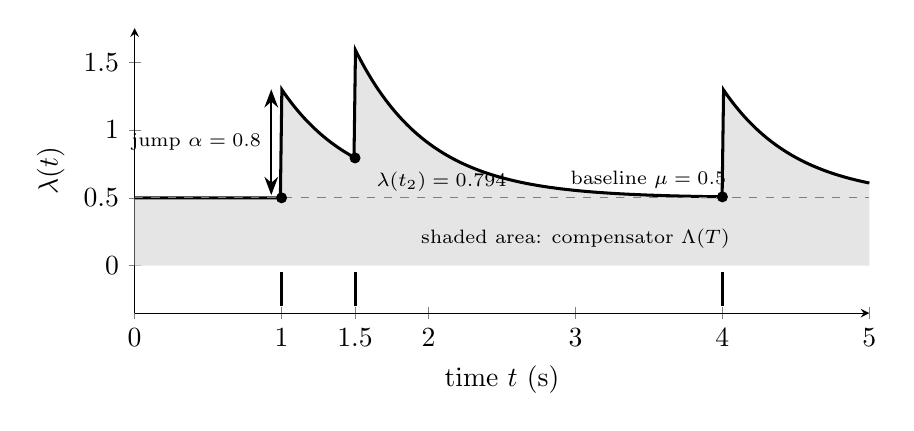
\begin{tikzpicture}
\begin{axis}[width=0.9\linewidth,height=5.2cm,xmin=0,xmax=5,ymin=-0.35,ymax=1.75,
  axis lines=left,xlabel={time $t$ (s)},ylabel={$\lambda(t)$},
  ytick={0,0.5,1,1.5},xtick={0,1,1.5,2,3,4,5},
  every axis plot/.append style={line width=1.1pt},clip=false]
  \addplot[name path=lam,color=black,samples=500,domain=0:5]
    {0.5+(x>1)*0.8*exp(-2*max(x-1,0))+(x>1.5)*0.8*exp(-2*max(x-1.5,0))+(x>4)*0.8*exp(-2*max(x-4,0))};
  \addplot[name path=zero,draw=none,domain=0:5]{0};
  \addplot[gray!20] fill between[of=lam and zero];
  \addplot[gray,dashed,thin,domain=0:5]{0.5};
  \node[font=\scriptsize,anchor=south west] at (axis cs:2.9,0.5) {baseline $\mu=0.5$};
  \foreach \t/\l in {1/0.5,1.5/0.794,4/0.507}{
    \edef\temp{\noexpand\draw[line width=1.1pt] (axis cs:\t,-0.3) -- (axis cs:\t,-0.05);
      \noexpand\fill (axis cs:\t,\l) circle (2pt);}
    \temp}
  \node[font=\scriptsize,anchor=north west] at (axis cs:1.58,0.76) {$\lambda(t_2)=0.794$};
  \draw[{Stealth}-{Stealth},thick] (axis cs:0.93,1.30) -- node[left,font=\scriptsize]{jump $\alpha=0.8$} (axis cs:0.93,0.52);
  \node[font=\scriptsize,align=center] at (axis cs:3.0,0.2) {shaded area: compensator $\Lambda(T)$};
\end{axis}
\end{tikzpicture}
\caption{Intensity of a univariate Hawkes process with \(\mu=0.5\), \(\alpha=0.8\) and
\(\beta=2\), for three events (ticks on the axis). Each event adds a jump that decays with
half-life \(\ln 2/2\approx0.35\)~s. The dots are the intensities at the events, the terms
that the likelihood rewards; the shaded area is the compensator, the term it penalizes.}
\label{fig:intensity}
\end{figure}

\paragraph{The intensity as a state.} Write \(E(t)=\lambda(t)-\mu\) for the excitation.
Between events, \(E\) decays as \(\mathrm dE/\mathrm dt=-\beta E\); at an event it jumps by
\(\alpha\). Hence, with \(\Delta_k=t_k-t_{k-1}\),
\begin{equation}
  E(t_k^-)=e^{-\beta\Delta_k}\bigl(E(t_{k-1}^-)+\alpha\bigr),
  \label{eq:recursion}
\end{equation}
and the current intensity summarizes the whole past: with an exponential kernel the
process \(\lambda(t)\) is Markov. This property makes simulation and the likelihood linear
in the number of events. It does not hold for other kernels, such as the power law, where
the whole history must be kept.

\paragraph{Cluster representation.} The same process can be generated as a population
\citep{hawkes2018,laub2021}. Immigrants arrive as a Poisson process of rate \(\mu\); each
event, immigrant or not, produces children as an inhomogeneous Poisson process of rate
\(\alpha e^{-\beta s}\), where \(s\) is the time since the parent. The number of direct
children of an event is Poisson with mean
\[
  g=\int_0^\infty\alpha e^{-\beta s}\,\mathrm ds=\frac{\alpha}{\beta},
\]
which is why \(g\) is called the branching ratio. Children, grandchildren and further
generations form a geometric series, so the mean size of the cluster started by one
immigrant is
\[
  1+g+g^2+\cdots=\frac{1}{1-g}\qquad(g<1),
\]
and a fraction \(g\) of all events is endogenous, triggered by earlier events rather than by
the baseline. Taking expectations in Equation~\eqref{eq:hawkes1d}, the stationary mean rate
\(\bar\lambda=\E[\lambda(t)]\) satisfies \(\bar\lambda=\mu+g\bar\lambda\), that is,
\(\bar\lambda=\mu/(1-g)\). Only the times are observed; the genealogy
(Figure~\ref{fig:cluster}) is latent.

\begin{figure}[htbp]
\centering
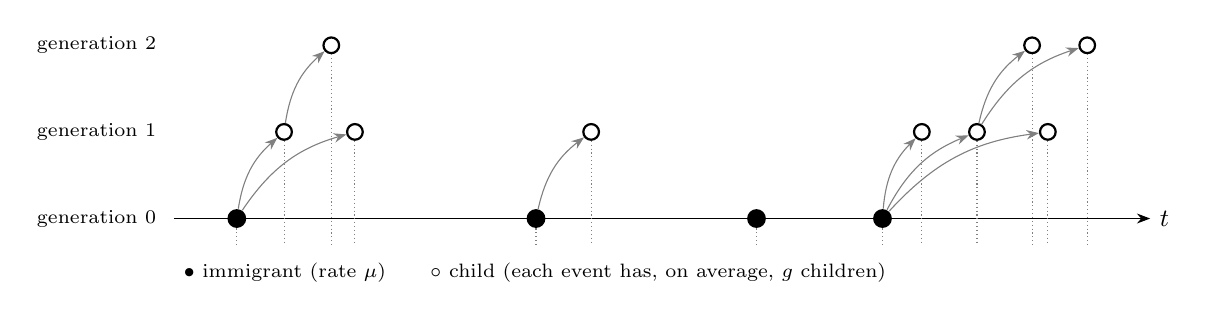
\begin{tikzpicture}[x=1.0cm,y=1.1cm,
  imig/.style={circle,fill=black,inner sep=2.4pt},
  child/.style={circle,draw=black,fill=white,thick,inner sep=2pt},
  link/.style={-{Stealth[length=1.6mm]},gray,thin}]
  \draw[-{Stealth}] (0,0) -- (12.4,0) node[right,font=\small]{$t$};
  \node[imig] (a) at (0.8,0) {};
  \node[child] (a1) at (1.4,1) {}; \node[child] (a2) at (2.3,1) {};
  \node[child] (a11) at (2.0,2) {};
  \draw[link] (a) to[bend left=20] (a1); \draw[link] (a) to[bend left=20] (a2);
  \draw[link] (a1) to[bend left=20] (a11);
  \node[imig] (b) at (4.6,0) {};
  \node[child] (b1) at (5.3,1) {};
  \draw[link] (b) to[bend left=20] (b1);
  \node[imig] (c) at (7.4,0) {};
  \node[imig] (d) at (9.0,0) {};
  \node[child] (d1) at (9.5,1) {}; \node[child] (d2) at (10.2,1) {}; \node[child] (d3) at (11.1,1) {};
  \node[child] (d21) at (10.9,2) {}; \node[child] (d22) at (11.6,2) {};
  \draw[link] (d) to[bend left=20] (d1); \draw[link] (d) to[bend left=20] (d2); \draw[link] (d) to[bend left=20] (d3);
  \draw[link] (d2) to[bend left=20] (d21); \draw[link] (d2) to[bend left=20] (d22);
  \foreach \p in {a,a1,a2,a11,b,b1,c,d,d1,d2,d3,d21,d22}{\draw[densely dotted,gray] (\p) -- (\p|-{(0,-0.3)});}
  \foreach \y in {0,1,2}{\node[font=\scriptsize,anchor=east] at (-0.1,\y) {generation \y};}
  \node[font=\scriptsize,anchor=north west] at (0,-0.4) {$\bullet$ immigrant (rate $\mu$)\qquad
    $\circ$ child (each event has, on average, $g$ children)};
\end{tikzpicture}
\caption{Cluster representation of a Hawkes process. Only the projection of the events on
the time axis is observed; which event triggered which is hidden. With \(g=0.5\), each
immigrant brings on average a cluster of \(1/(1-0.5)=2\) events.}
\label{fig:cluster}
\end{figure}

\section{Symmetric bivariate Hawkes process}

A \(D\)-dimensional Hawkes process has one intensity per type,
\[
 \lambda_i(t)=\mu_i+\sum_{j=1}^{D}\int_{(0,t)}\phi_{ij}(t-s)\,\mathrm dN_j(s),
 \qquad i=1,\dots,D,
\]
where \(\phi_{ij}\) is the effect of a type-\(j\) event on the intensity of type \(i\)
\citep{hawkes1971b,bacry2015}. With exponential kernels and two types there are, in general,
two baselines, four jump sizes and up to four decay rates. Here,
up-moves and down-moves are processes \(N_1,N_2\) with a common decay and symmetric
excitation:
\begin{align}
\lambda_1(t)&=\mu+\sum_{t_k^1<t}\alpha_{\mathrm{self}}e^{-\beta(t-t_k^1)}
 +\sum_{t_k^2<t}\alpha_{\mathrm{cross}}e^{-\beta(t-t_k^2)},\\
\lambda_2(t)&=\mu+\sum_{t_k^2<t}\alpha_{\mathrm{self}}e^{-\beta(t-t_k^2)}
 +\sum_{t_k^1<t}\alpha_{\mathrm{cross}}e^{-\beta(t-t_k^1)}.
\end{align}
The model reduces a general matrix to four parameters. This parsimony makes
simulation and comparison with \citet{lee2023} easier. Figure~\ref{fig:bivariate} draws it
as a diagram of the two event types. An up-move raises the intensity of another up-move by
\(\alpha_{\mathrm{self}}\) and that of a down-move by \(\alpha_{\mathrm{cross}}\), and
symmetrically for a down-move; both increases decay at the same rate \(\beta\). In
microstructure, dominant cross-excitation indicates reversion (an up-move followed by a
down-move), and dominant self-excitation indicates persistence of direction
\citep{bacry2013}.

\begin{figure}[htbp]
\centering
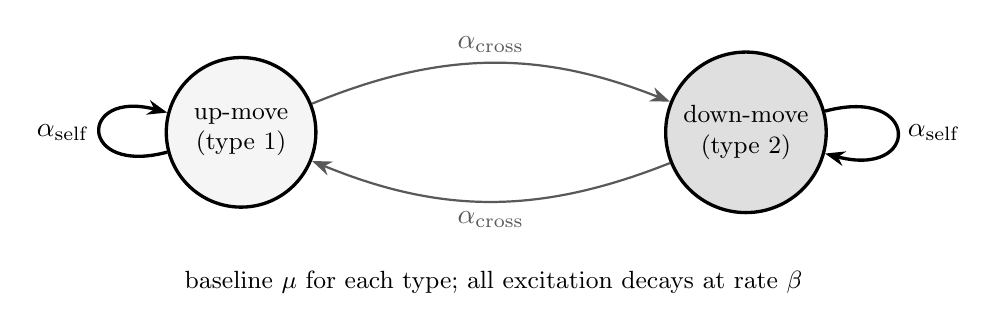
\begin{tikzpicture}[node distance=4.4cm,
  ev/.style={circle,draw=black,very thick,minimum size=1.9cm,font=\small,align=center}]
  \node[ev,fill=gray!8] (u) {up-move\\(type 1)};
  \node[ev,fill=gray!25,right=of u] (d) {down-move\\(type 2)};
  \draw[-{Stealth[length=2.5mm]},very thick] (u) edge[loop left,looseness=6]
    node[left]{$\alpha_{\mathrm{self}}$} (u);
  \draw[-{Stealth[length=2.5mm]},very thick] (d) edge[loop right,looseness=6]
    node[right]{$\alpha_{\mathrm{self}}$} (d);
  \draw[-{Stealth[length=2.5mm]},thick,gray!70!black] (u) to[bend left=22]
    node[above]{$\alpha_{\mathrm{cross}}$} (d);
  \draw[-{Stealth[length=2.5mm]},thick,gray!70!black] (d) to[bend left=22]
    node[below]{$\alpha_{\mathrm{cross}}$} (u);
  \node[font=\small] at ($(u)!0.5!(d)+(0,-1.9)$) {baseline $\mu$ for each type; all excitation decays at rate $\beta$};
\end{tikzpicture}
\caption{The symmetric bivariate Hawkes process as a diagram of event types. Loops are
self-excitation, arrows between types are cross-excitation; the same four parameters
\((\mu,\alpha_{\mathrm{self}},\alpha_{\mathrm{cross}},\beta)\) apply to both types.
\(\alpha_{\mathrm{self}}>\alpha_{\mathrm{cross}}\) describes persistence of direction, as
found in the crypto data of this work; \(\alpha_{\mathrm{cross}}>\alpha_{\mathrm{self}}\)
describes reversion, as at the equity fixed point of \citet{lee2023}.}
\label{fig:bivariate}
\end{figure}

\section{Stability}

The mass matrix of the kernels is
\[
 \mathbf G=\frac{1}{\beta}
 \begin{bmatrix}
  \alpha_{\mathrm{self}} & \alpha_{\mathrm{cross}}\\
  \alpha_{\mathrm{cross}} & \alpha_{\mathrm{self}}
 \end{bmatrix}.
\]
Its entry \((i,j)\) is the mean number of type-\(i\) children of a type-\(j\) event, so
\(\mathbf G\) plays the role of the branching ratio. Its eigenvalues are
\((\alpha_{\mathrm{self}}-\alpha_{\mathrm{cross}})/\beta\) and the largest,
\[
 g=\frac{\alpha_{\mathrm{self}}+\alpha_{\mathrm{cross}}}{\beta},
\]
which is the mean number of children of either type per event. The two eigenvalues have
eigenvectors \((1,1)\) and \((1,-1)\): the first governs the total activity
\(N_1+N_2\), the second the difference \(N_1-N_2\), that is, the price
(Section~\ref{sec:volatility-theory}). Write
\[
 g_-=\frac{\alpha_{\mathrm{self}}-\alpha_{\mathrm{cross}}}{\beta}
\]
for the second eigenvalue. The condition \(g<1\) is
required. Close to one, cascades last longer; above one, there is no usual stationary
regime \citep{hardiman2013,filimonov2012}. Under stationarity, by the same argument as in
the univariate case, each type occurs at mean rate \(\mu/(1-g)\), and the two together at
\(2\mu/(1-g)\).

\section{Marks and price}

An event has a time, a type and a mark. The mark is the size of the change in ticks.
The paper keeps the mark for volatility, but assumes that the intensity does not
depend on it. The filtered price can be written, in ticks, as the cumulative
difference between up-moves and down-moves.

\section{Volatility}
\label{sec:volatility-theory}

In a minimal model, if the price moves by one tick \(\vartheta\) at a rate \(\phi\),
\[
 \sigma^2\approx\phi\vartheta^2.
\]
Thus, modeling intensity is modeling activity and, consequently, a component of
volatility. The marked Hawkes expression requires moments of the marks and the
estimated parameters \citep{leeseo2017,lee2024}.

\paragraph{Long-run variance of the Hawkes price.} With unit marks the price is
\(X(t)=N_1(t)-N_2(t)\), the projection on the eigenvector \((1,-1)\). Under stationarity each
type has mean rate \(\bar\lambda=\mu/(1-g)\), and the variance of \(X\) per unit time
converges, as the horizon grows, to
\[
 \lim_{T\to\infty}\frac{\Var X(T)}{T}=\frac{2\bar\lambda}{(1-g_-)^2}
\]
\citep{bacry2013}. If each event moves the price by an i.i.d.\ size \(J\), independent of the
times, with the sign given by the type, the same argument gives
\begin{equation}
 \sigma_H^2=2\bar\lambda\left[\Var(J)+\frac{\E[J]^2}{(1-g_-)^2}\right],
 \label{eq:hawkes-variance}
\end{equation}
the expression used in Section~\ref{sec:real-volatility}. The total activity depends on
\(g\), and the amplification of the variance on \(g_-\). When self-excitation dominates,
\(g_->0\) and moves in the same direction cluster, so the variance exceeds that of a Poisson
price with the same activity. When cross-excitation dominates, \(g_-<0\), moves tend to undo
each other and the variance falls below it; this is the mechanism that \citet{bacry2013} use
to model microstructure noise. When \(\alpha_{\mathrm{self}}=\alpha_{\mathrm{cross}}\), the
long-run variance equals that of the difference of two independent Poisson processes with the
same activity.

\paragraph{Realized volatility.} The benchmark is the realized variance over a window,
\[
 \mathrm{RV}_\Delta=\sum_k r_k^2,
\]
the sum of squared log returns sampled every \(\Delta\) seconds
\citep{andersen2003,barndorff2002}. Without noise, it converges to the integrated variance as
\(\Delta\to0\). At high frequency, however, the observed price contains microstructure noise,
and \(\mathrm{RV}_\Delta\) is biased upward when \(\Delta\) is small \citep{zhang2005}. The
signature plot, \(\mathrm{RV}_\Delta\) per unit time against \(\Delta\), shows the effect:
noise makes it fall with \(\Delta\), while positively autocorrelated returns, as in a
self-exciting price, make it rise toward the long-run level of
Equation~\eqref{eq:hawkes-variance}.

\section{Simulation}

A Hawkes path can be simulated by Ogata's thinning \citep{ogata1981}. If
\(\lambda(t)\le M\) on an interval, candidates are drawn from a Poisson process of rate
\(M\) and each candidate at time \(s\) is kept with probability \(\lambda(s)/M\); the kept
points have intensity \(\lambda\). With an exponential kernel the intensity only decreases
between events, so its value just after the last event is a valid bound until the next
event. In the bivariate case the bound is \(\lambda_1+\lambda_2\), and the type of an
accepted event is drawn in proportion to \(\lambda_1\) and \(\lambda_2\). The
implementation is described in Section~\ref{sec:sim-thinning}.

\section{Maximum likelihood}
\label{sec:mle-theory}

For a horizon \(T\),
\[
 \ell(\theta)=\sum_k\log\lambda_{c_k}(t_k)
 -\sum_i\int_0^T\lambda_i(u)\,du.
\]
The first term rewards high intensity at the events; the second penalizes high
intensity over the whole interval. Maximizing only the first would drive the
intensities to infinity. The compensator provides the balance. For an exponential
kernel, the sum over the past obeys a first-order recursion, and \(\ell\) and its
gradient can be computed in \(O(n)\) operations \citep{ozaki1979}. In the univariate case,
let \(A_1=0\) and \(A_k=e^{-\beta(t_k-t_{k-1})}(1+A_{k-1})\), so that \(\alpha A_k\) is
the excitation just before \(t_k\) (Equation~\eqref{eq:recursion}). Then
\begin{equation}
 \ell(\mu,\alpha,\beta)=\sum_{k=1}^{n}\log\bigl(\mu+\alpha A_k\bigr)-\mu T
 -\frac{\alpha}{\beta}\sum_{k=1}^{n}\Bigl(1-e^{-\beta(T-t_k)}\Bigr).
 \label{eq:loglik1d}
\end{equation}
The bivariate likelihood has the same structure, with one recursion per pair of source and
target types. Under regularity conditions, the MLE is consistent and asymptotically
efficient \citep{ogata1978}: approximately normal around the true value, with covariance
given by the inverse Fisher information, which the inverse of the observed Hessian of
\(-\ell\) estimates. These conditions include a true parameter in the interior of the
parameter space. When it lies on the boundary, as \(\alpha_{\mathrm{cross}}=0\), the
estimate piles up at the boundary with positive probability, and neither the normal
approximation nor the usual \(\chi^2\) reference for likelihood ratio tests applies
\citep{selfliang1987}. This is relevant for the real data of this work, where
\(\alpha_{\mathrm{cross}}\) is estimated close to zero.

\section{Model comparison}

The Poisson process is nested in the Hawkes process: it is the case
\(\alpha_{\mathrm{self}}=\alpha_{\mathrm{cross}}=0\). The likelihood ratio statistic
\(2(\hat\ell_{\mathrm{Hawkes}}-\hat\ell_{\mathrm{Poisson}})\) measures the gain in fit. Its
usual \(\chi^2\) reference does not hold here for two reasons: the null value lies on the
boundary of the parameter space \citep{selfliang1987}, and \(\beta\) has no effect under the
null, so it is not identified there. The Akaike information criterion,
\[
 \mathrm{AIC}=2k-2\hat\ell,
\]
with \(k\) the number of free parameters, compares the two fits with a penalty for the extra
parameters \citep{akaike1974}. A difference in AIC of hundreds of units, as found on the real
windows, leaves no doubt about the direction, whatever the exact reference distribution.

\section{Goodness of fit by time rescaling}
\label{sec:time-rescaling}

If the model is correct, the compensator turns the observed process into a unit-rate
Poisson process: the transformed times \(\Lambda(t_k)\) are the events of a homogeneous
Poisson process of rate one. This is the time-rescaling theorem \citep{brown2002}. The
increments
\[
 \tau_k=\Lambda(t_k)-\Lambda(t_{k-1})=\int_{t_{k-1}}^{t_k}\lambda(u)\,\mathrm du
\]
are then independent \(\mathrm{Exp}(1)\) variables. In the bivariate case the theorem
applies to each type with its own compensator \(\Lambda_i\). Evaluated at the estimated
parameters, the \(\tau_k\) are the rescaled residuals of the fit \citep{ogata1988}. Their
distribution is tested against \(\mathrm{Exp}(1)\), for example with Kolmogorov--Smirnov,
and their serial dependence with Ljung--Box. A kernel of the wrong shape typically leaves
dependence in the residuals: bursts that the fitted kernel forgets too fast or too slowly
appear as runs of short or long \(\tau_k\).

\section{Observation on a time grid}

The events of this work are changes of the mid-price recorded on a 100~ms grid
(Chapter~\ref{cap:dados}). Two things are lost relative to continuous time: event times are
rounded to the grid, and changes that fall in the same cell merge into one. The second
matters most for the decay. With \(\beta\) of a few units per second, much of the excitation
acts within a few hundred milliseconds, and merged events remove part of the short
inter-arrivals from which \(\beta\) is identified. A likelihood written for continuous time
therefore estimates the parameters of the process as seen through the grid, with \(\beta\)
biased downward; Section~\ref{sec:addendum-grid} measures the size of this bias.
Likelihoods that account for the observation scheme have been proposed for this setting
\citep{lambe2025}.

A biased estimator can still be corrected by simulation, the idea of indirect inference
\citep{gourieroux1993}. Let \(b(\theta)\) be a summary, such as the median, of the grid MLE
over paths simulated from \(\theta\) in continuous time and mapped to the grid. The map
\(b\) is estimated by simulation, and an estimate on the grid is corrected by solving
\(b(\theta)=\hat\theta_{\mathrm{grid}}\). The correction is as good as the model used to
simulate: if the real process is not a Hawkes process, the map transfers its bias with it.
A network trained on gridded paths with the continuous-time parameter as target learns a
correction of the same kind, conditional on the whole path.

\section{Identifiability in finite samples}
\label{sec:identificabilidade}

The asymptotic properties do not guarantee good behavior with 1,000 events. When the
excitation is weak (small \(\alpha_{\mathrm{self}}+\alpha_{\mathrm{cross}}\)), the
kernel barely changes the intensity, and the likelihood becomes flat in the direction
of \(\beta\): very different values of \(\beta\) explain the data almost equally well.
In the limit \(\alpha\to0\), \(\beta\) is no longer identified. Near criticality, the
separation between \(\mu\) and \(g\) also deteriorates, because the mean rate
\(2\mu/(1-g)\) is well determined, but neither factor is on its own. These effects
reappear in the results of Chapter~\ref{cap:resultados}.

\section{Amortized estimation as a Bayes estimator}
\label{sec:bayes}

In the approach of \citet{lee2023}, a network \(f_\phi\) is trained on pairs
\((\theta_i,x_i)\), where \(\theta_i\) is drawn from a training distribution \(\pi\)
and \(x_i\) is simulated from the model with parameter \(\theta_i\). Minimizing the
mean squared error,
\[
  \min_\phi\;\E_{\theta\sim\pi}\,\E_{x\mid\theta}
  \bigl\lVert f_\phi(x)-\theta\bigr\rVert^2,
\]
is minimizing the Bayes risk under squared loss, whose solution is the posterior mean
\(\E_\pi[\theta\mid x]\) \citep{lehmann1998}. Hence, a well-trained network
approximates a Bayes estimator under the prior \(\pi\)
\citep{sainsburydale2024,lenzi2023}. Two consequences guide this work. First, on a
test set drawn from the same \(\pi\), no estimator has lower average MSE than the
posterior mean, so outperforming the MLE on that test is expected and does not prove
superiority in a frequentist sense. Second, the network does not extrapolate: its
estimates shrink toward the high-density region of \(\pi\), and real data outside the
support of the prior yield biased estimates.

The same approach belongs to a wider family of amortized, simulation-based inference methods,
in which the cost of inference is paid once, in training, and each new data set costs a
forward pass \citep{cranmer2020,radev2022}. On real windows the target changes. When a
network is trained on pairs \((x,\hat\theta_{\mathrm{MLE}}(x))\), the label is a deterministic
function of the input, so the minimizer of the squared loss is the MLE itself: the network
becomes a fast approximation of the MLE map, accurate where the training windows are dense.
Starting from the weights trained on simulated data, it can reach that approximation with
fewer real windows; how close the simulation prior is to the real data then matters for how
much that initialization helps.

\section{Comparing estimators}
\label{sec:comparing-theory}

The estimators are compared path by path. For each path or window \(i\), a loss
\(L_i(A)\), such as the squared error averaged over the four parameters, is computed for each
estimator \(A\); the macro MSE is the average of the per-parameter MSEs. Two estimators are
compared through the paired differences \(d_i=L_i(A)-L_i(B)\). Pairing removes the variation
in difficulty between paths, which is often much larger than the difference between
estimators.
The mean \(\bar d\) is reported with a bootstrap confidence interval, obtained by resampling
the \(d_i\) with replacement \citep{efron1993}, and the null hypothesis of no difference is
tested with the Wilcoxon signed-rank test, which uses the ranks of \(|d_i|\) and is robust to
the heavy tails of squared errors \citep{wilcoxon1945,diebold1995}. Variation across training
seeds is a different source: it measures the instability of training, not the accuracy of a
trained model, and is compared across seeds \citep{bouthillier2021}.

When several comparisons are tested together, the Holm procedure controls the probability
of any false rejection: with the \(m\) \(p\)-values sorted in increasing order, the \(k\)-th
is compared with \(0.05/(m-k+1)\), and testing stops at the first non-rejection
\citep{holm1979}. Agreement between two orderings, such as the Hawkes and the realized
volatilities across windows, is measured by the Spearman correlation, the correlation of the
ranks, which ignores the level and depends only on the order.

\paragraph{Ensembles.} The average \(\bar y=\frac1M\sum_m y_m\) of \(M\) estimators satisfies
\[
 \lVert\bar y-\theta\rVert^2=\frac1M\sum_{m=1}^{M}\lVert y_m-\theta\rVert^2
 -\frac1M\sum_{m=1}^{M}\lVert y_m-\bar y\rVert^2
\]
\citep{krogh1995}. The error of the average equals the average error of the members minus
their spread, so it is never worse than the average member, and it improves most when the
members are accurate and err in different places. This identity applies both to the
ensembles of five seeds and to the average of the LSTM and the Transformer.

\section{LSTM}

Recurrent networks update a state \(h_t=f(x_t,h_{t-1})\). The LSTM introduces input,
forget and output gates to control the flow of information and mitigate the
vanishing gradient problem \citep{hochreiter1997}. With \(\sigma\) the logistic function
and \(\odot\) the elementwise product,
\begin{align*}
 f_t&=\sigma(W_f[h_{t-1},x_t]+b_f), & i_t&=\sigma(W_i[h_{t-1},x_t]+b_i),\\
 o_t&=\sigma(W_o[h_{t-1},x_t]+b_o), & \tilde c_t&=\tanh(W_c[h_{t-1},x_t]+b_c),\\
 c_t&=f_t\odot c_{t-1}+i_t\odot\tilde c_t, & h_t&=o_t\odot\tanh(c_t).
\end{align*}
The cell state \(c_t\) is updated additively, which lets gradients pass over many steps.
The update has the form of Equation~\eqref{eq:recursion}: a forget gate that depends on the
inter-arrival time can play the role of \(e^{-\beta\Delta_k}\), and the input gate that of
the jump, so an LSTM can represent the excitation of a Hawkes process in its state. In
Lee, the sequence contains the inter-arrival time and the type; the final state feeds the
regression of the four parameters. The paper also tested a GRU \citep{cho2014}, with
slightly worse results.

\section{Attention and the Transformer}

Attention computes weighted combinations:
\[
 \operatorname{Attention}(Q,K,V)=
 \operatorname{softmax}\left(\frac{QK^\top}{\sqrt{d_k}}\right)V.
\]
Each position queries all the others. The Transformer combines multiple heads,
feed-forward layers, residual connections and normalization \citep{vaswani2017}. Each head
applies its own projections \(Q=XW^Q\), \(K=XW^K\), \(V=XW^V\) to the sequence \(X\), and
the heads are concatenated. Self-attention is equivariant to permutations of the sequence,
so order and spacing must enter through a positional encoding; for a point process the
relevant position is the time of each event, not only its index. The
potential advantage is capturing distant dependencies; the potential cost is
\(O(n^2)\) memory. The position of the normalization relative to the residual
connections affects training stability: the \emph{post-LN} variant, used here,
usually requires learning-rate warm-up \citep{xiong2020}.

\section{Training}

The networks are trained by stochastic gradient descent on mini-batches with Adam, which
scales each step by running estimates of the first and second moments of the gradient
\citep{kingma2015}. The learning rate can follow a schedule, such as a short warm-up or a cosine decay
\citep{xiong2020,loshchilov2017}. Training stops at a fixed budget of epochs or when the
validation loss stops improving, and the checkpoint with the lowest validation loss is kept;
the test data are not used for any choice. Fine-tuning reuses this procedure from weights
already trained on another task, here the simulated paths, with the real windows as the new
training set.

\chapter{Related Work}

\section{Hawkes processes in finance}

After the original formulation \citep{hawkes1971,hawkes1971b}, self- and mutually
exciting models came to describe market events in continuous time
\citep{bowsher2007,embrechts2011}, contagion between markets \citep{aitsahalia2015}
and endogeneity, measured by the branching ratio \citep{filimonov2012,hardiman2013}.
\citet{bacry2013} use a bivariate Hawkes process of up- and down-moves to reproduce
the microstructure noise of the price; cross-excitation captures reversion at short
scales. \citet{bacry2015} and \citet{hawkes2018} review this field, and
\citet{mutoke2011} offers a didactic introduction. \citet{leeseo2017} connect the
marked Hawkes process to the price in ticks and derive Hawkes volatility, which
\citet{lee2024} apply to filtered prices. In Brazil, \citet{primo2018} analyzes the
intraday clustering of stocks with MLE, and \citet{silva2026} systematizes inference,
diagnostics and financial applications.

\section{Estimation of Hawkes processes}

MLE for exponential kernels dates back to \citet{ozaki1979}, with asymptotic
properties established by \citet{ogata1978}. Simulation by \emph{thinning}
\citep{ogata1981} and diagnostics by rescaled residuals \citep{ogata1988,brown2002}
complete the classical toolbox \citep{laub2021}. The optimization is sensitive to the
initialization and to the geometry of the likelihood, which can be nearly flat in
some directions when the series is short (Section~\ref{sec:identificabilidade}).

\section{Amortized and simulation-based inference}

When the likelihood is expensive or intractable, networks trained on simulations
replace the optimization with a single forward pass \citep{cranmer2020}. Networks
trained on simulations already estimate parameters of spatial and extreme-value
models \citep{gerber2021,lenzi2023}; with squared loss, they approximate Bayes
estimators \citep{sainsburydale2024}, and methods such as BayesFlow learn the full
posterior \citep{radev2022}. \citet{lee2023} applies the idea to the 2D Hawkes process
with an LSTM. \citet{lambe2025} use networks for the Hawkes process observed only
through interval counts, a case in which the exact likelihood is intractable and the
MLE is no longer a direct alternative.

\section{Neural point processes}

Another line of work uses networks to model the intensity itself, without the
parametric form of Hawkes: RMTPP \citep{du2016}, the Neural Hawkes Process
\citep{mei2017} and attention-based variants such as the Transformer Hawkes Process
\citep{zuo2020} and the Self-Attentive Hawkes Process \citep{zhang2020};
\citet{shchur2021} review the area. The goal differs from that of this work: those
models maximize predictive likelihood, whereas here the network estimates the four
interpretable parameters of a classical model.

\section{Hawkes processes in crypto-assets}

Using one-minute returns of 17 cryptocurrencies traded on Binance,
\citet{taddeo2024} show that Hawkes describes the occurrence of jumps in log-returns
better than Poisson. The crypto market also exhibits segmentation and limited
arbitrage across exchanges \citep{makarov2020}, and perpetual futures, which have no
expiry and carry a funding rate, concentrate a large share of the liquidity
\citep{he2022perpetual}.

\section{Positioning}

\begin{table}[htbp]
\centering
\caption{Positioning of this work relative to the closely related literature.}
\label{tab:posicionamento}
\small
\begin{tabularx}{\linewidth}{lllX}
\toprule
Work & Estimation & Architecture & Market\\
\midrule
\citet{bacry2013} & MLE & -- & futures (Bund, DAX)\\
\citet{leeseo2017} & MLE & -- & equities\\
\citet{primo2018} & MLE & -- & equities (Brazil)\\
\citet{taddeo2024} & MLE & -- & crypto (jumps in 1-min returns)\\
\citet{lee2023} & network & LSTM & equities (US)\\
\citet{lambe2025} & network & MLP & synthetic (counts)\\
\citet{zuo2020} & neural intensity & Transformer & generic\\
This work & network and MLE & LSTM and Transformer & crypto (perpetual futures)\\
\bottomrule
\end{tabularx}
\end{table}

The present work combines controlled reproduction, public crypto data and a
comparison with attention, and adds to the evaluation of \citet{lee2023} robust
metrics, paired tests and the interpretation of the network as a Bayes estimator.

\chapter{Data}
\label{cap:dados}

\section{Source and market}

Both spot and futures were evaluated. The need for the best bid/ask ruled out the
official spot archive, which has no equivalent historical \dataset{bookTicker}. USD-M
futures provide \dataset{bookTicker} and \dataset{aggTrades}. The symbols are BTCUSDT
and ETHUSDT \citep{binancePublicData}.

\section{Schema}

\dataset{bookTicker} includes an identifier, the best bid and ask prices and
quantities, the transaction time and the event time. The canonical schema has a UTC
timestamp, bid, ask and quantities. Audits check for positive prices, bid less than
or equal to ask, ordering and temporal duplicates.

\section{Sampling}

Updates can occur every millisecond, a much finer resolution than the chosen scale.
Timestamps are grouped into 100 ms bins and the last state is kept. This filter
follows Lee's protocol and reduces ultra-high-frequency noise.

\section{Datasets produced}

\begin{table}[htbp]
\centering
\caption{Dataset coverage.}
\label{tab:cobertura}
\begin{tabular}{lrrr}
\toprule
Window & Symbol-days & Events & Segments of 1,000\\
\midrule
Primary (Jan.\ 2024) & 28 & 1,826,904 & 1,813\\
Robustness (Oct.\ 2023) & 14 & 1,288,352 & 1,281\\
\bottomrule
\end{tabular}
\end{table}

\section{Event characteristics}
\label{sec:caracteristicas}

Table~\ref{tab:caracteristicas} summarizes the events of the calibration block
(January 15 to 22, 2024). Three facts distinguish these data from the setting of
\citet{lee2023}. First, about 76\% of the changes repeat the direction of the previous
one, which indicates persistence rather than reversion. Second, the median jump is 10
to 15 ticks and only 10--13\% of the jumps are one tick: at the 100~ms scale, these
contracts behave as small-tick assets. Third, 37--39\% of the inter-arrival times are
exactly 0.1~s, the grid step; the sampling strongly discretizes the times, whereas the
model and the simulations assume continuous time.

\begin{table}[htbp]
\centering
\caption{Characteristics of the mid-price events, January 15 to 22, 2024.}
\label{tab:caracteristicas}
\small
\begin{tabular}{lrr}
\toprule
 & BTCUSDT & ETHUSDT\\
\midrule
Events & 529,278 & 540,164\\
Fraction of up-moves & 49.4\% & 49.5\%\\
Probability of repeating the previous direction & 76.0\% & 75.7\%\\
Median inter-arrival time & 0.3 s & 0.3 s\\
Inter-arrival times equal to 0.1 s (grid) & 39.5\% & 37.3\%\\
Median / 90th percentile jump (ticks) & 15.5 / 48 & 10 / 29\\
One-tick jumps & 9.7\% & 12.6\%\\
\bottomrule
\end{tabular}
\end{table}

\chapter{Methodology}

\section{Principles}

The protocol distinguishes:
\begin{description}
  \item[R1:] explicitly published information;
  \item[R2:] reconstruction to fill a gap;
  \item[A1:] adaptation required for crypto;
  \item[E1:] extension with a Transformer.
\end{description}

\section{Pipeline}

\begin{enumerate}
  \item build the daily URL and download the ZIP;
  \item compute the SHA-256 and record it in a manifest;
  \item temporarily extract the CSV;
  \item process chunks of one million rows;
  \item reduce the updates to the 100 ms grid;
  \item produce Parquet partitioned by symbol and date;
  \item delete the temporary CSV;
  \item create windows without crossing splits;
  \item fit the MLE and calibrate ranges on the training set only;
  \item generate synthetic paths and train the estimators;
  \item select hyperparameters on the validation set;
  \item open the test set only once.
\end{enumerate}

\section{Simulation by thinning}
\label{sec:sim-thinning}

Given the current state, an upper bound on the sum of the intensities is computed. An
exponential waiting time is drawn; the excitation decays; the candidate is accepted
with probability proportional to the new intensity \citep{ogata1981}. The type is
drawn with probabilities proportional to \(\lambda_1,\lambda_2\). After the event, the
corresponding column of the \(\alpha\) matrix is added. Each path starts with an
empty history, the same assumption as in the likelihood.

\section{Constrained MLE}

Positive parameters are obtained through softplus. Instead of optimizing \(\beta\)
freely, a positive margin \(d\) is used:
\[
(\mu,\alpha_s,\alpha_c,d)=\softplus(z),\qquad
\beta=\alpha_s+\alpha_c+d.
\]
L-BFGS-B is started from five points: one based on the empirical event rate and four
random perturbations in the unconstrained space. The MLE never receives the true
parameter as initialization. The gradient is analytic, and the exponential
recursions are solved as bidiagonal systems. Convergence, iterations, log-likelihood
and time are recorded.

\section{Neural protocol}

The target is \((\mu,\alpha_s,\alpha_c,\beta)\), and the loss is the MSE on the
original scale. The input for each event is \((\log(1+\Delta t),\,s)\), with \(s=+1\)
for an up-move and \(s=-1\) for a down-move; Lee uses inter-arrival times and types
1/2, so this transformation is a reconstruction (R2). The two networks share the
output head: softplus produces \(\mu,\alpha_s,\alpha_c,d>0\) and
\(\beta=\alpha_s+\alpha_c+d\), which guarantees \(g<1\) by construction, as in Lee's
robust version.

The frozen synthetic experiment contains 75,000 training sequences, 10,000 validation
sequences and 15,000 test sequences, all of exactly 1,000 events. The parameters are
drawn with \(\mu\in[0.2,\,0.6]\), \(\beta\in[0.8,\,2.0]\), self-excited fraction
\(\alpha_s/(\alpha_s+\alpha_c)\in[0.2,\,0.8]\) and \(g\) balanced across three
strata: low \([0.10,\,0.35)\), intermediate \([0.35,\,0.70)\) and near-critical
\([0.70,\,0.95]\). Table~\ref{tab:treino} summarizes the training.

\begin{table}[htbp]
\centering
\caption{Training configuration and cost (five seeds per network, Apple Silicon Mac
with MPS).}
\label{tab:treino}
\small
\begin{tabular}{lrr}
\toprule
 & LSTM (R1/R2) & Transformer (E1)\\
\midrule
Architecture & 2 LSTM $\times$ 12 + dense & encoder, 2 layers, $d=32$\\
Heads / feed-forward & -- & 4 / 128\\
Trainable parameters & 2,068 & 25,700\\
Optimizer & Adam, $10^{-3}$ & Adam, $10^{-3}$\\
Effective batch & 64 & 8 (physical 4 with accumulation)\\
Maximum epochs / patience & 300 / 30 & 300 / 30\\
Best epoch (per seed) & 165, 164, 193, 239, 299 & 73, 42, 38, 60, 44\\
Training time per seed & 5.4--14.8 h & 16.6--28.8 h\\
Total time (5 seeds) & 41 h & 110 h\\
\bottomrule
\end{tabular}
\end{table}

The Transformer's tensor flow starts from \([B,L,2]\), with \(L=1000\). A linear
projection produces \([B,L,32]\), to which the positional encoding is added. In each
layer, the four heads operate in subspaces of dimension eight; the feed-forward block
expands 32 to 128 and returns to 32. Temporal averaging converts \([B,L,32]\) into
\([B,32]\). The memory cost of attention grows quadratically with \(L\), which is why
its batch is smaller than the LSTM's. This difference in batch size, together with the
absence of a hyperparameter search for either network, is a limitation of the
comparison.

\section{The paper's fixed point (E2)}

To compare directly with the sampling-distribution table of \citet{lee2023}, 2,000
paths of 1,000 events were simulated at the published point
\((\mu,\alpha_s,\alpha_c,\beta)=(0.3,\,0.4,\,0.7,\,1.5)\), which lies inside the
training prior. The networks were applied without retraining, and the MLE was fitted
in two versions: the protocol's heuristic and the initialization at the true value
used in the paper.

\section{Empirical protocol}
\label{sec:empirical-protocol}

On real data there is no true parameter, so the empirical stage asks three narrower
questions: whether the Hawkes model describes the windows well enough to be estimated, whether
a network can reproduce the MLE on real windows, and whether the estimated parameters give a
volatility consistent with the realized one. The protocol was fixed in a decision record
(ADR~008) before the test block was opened. The windows have 1,000 events and are split
chronologically by day: calibration (15--22 January 2024, 1,063 windows), validation (23--25
January, 476 windows) and test (26--28 January, 274 windows); the October 2023 week is a
robustness window that is never used for training or selection.

\paragraph{Goodness of fit.} With the MLE of each calibration window, the time-rescaled
residuals of each dimension are tested against \(\mathrm{Exp}(1)\) with Kolmogorov--Smirnov and
for serial dependence with Ljung--Box at 10 lags \citep{ogata1988,brown2002}, and the Hawkes
model is compared with a homogeneous bivariate Poisson process by likelihood ratio and AIC.
Since the times lie on a 100~ms grid, two controls separate the effect of the grid from
misspecification: times jittered uniformly inside their cell with the MLE refitted, and paths
simulated from each fitted model, either in continuous time or mapped to the grid in the same
way as the data. The rejection rate of the simulated controls is what a correct model would
produce.

\paragraph{Networks on real windows.} Each window is labeled with its MLE (five heuristic
starts). Both architectures are trained on the calibration labels with the loss, batch size,
maximum of 300 epochs and patience of 30 of the synthetic protocol, in two variants: from
scratch (Adam, \(10^{-3}\)) and fine-tuned from the synthetic weights of the same seed (Adam,
\(10^{-4}\)), each with the five protocol seeds. Two references need no training: the synthetic
networks as they are, and the mean of the training labels, which is the best constant
predictor. The selected variant is the one whose five-seed ensemble has the lowest macro MSE
on validation. The test block is labeled and read once, after the selection; the stored
weights are evaluated without retraining, and every variant is reported. The machine budget
for this stage was capped at 30 hours.

\paragraph{Volatility.} The long-run volatility implied by the estimated parameters
(Section~\ref{sec:real-volatility}) is compared window by window with the realized volatility
of the log mid-price sampled every \(\Delta\in\{0.1, 1, 5, 10, 30\}\) seconds, using the median
ratio and the Spearman correlation across windows, with \(\Delta=10\)~s as the main horizon,
for the MLE and for the selected network.

\section{Metrics and tests}

The reported metrics are per-parameter and aggregate MSE, median absolute error,
bias, validity, branching-ratio error, cost and MLE convergence. Because the
parameters have different scales, the \(R^2\) of each parameter relative to the prior
mean (the trivial estimator) is also reported. The comparison between networks uses
two sources of variation: across seeds (Welch and Mann--Whitney tests with five
seeds), which measures training variability \citep{bouthillier2021}, and across test
paths (paired difference with a \emph{bootstrap} CI and Wilcoxon test), which measures
the accuracy of the already trained models \citep{efron1993,diebold1995}.

\chapter{Results}
\label{cap:resultados}

\section{Data gate}

All 56 primary files were present. Twenty-eight partitions were generated. BTCUSDT
produced 887,803 events; ETHUSDT, 939,101. The independent window produced 1,288,352
events. The availability and volume gate was therefore satisfied.

\section{Reproduction at the fixed point}

\input{en/e2_fixed_point.tex}

Table~\ref{tab:e2-ponto-fixo} reproduces the qualitative pattern of \citet{lee2023}.
The MLE is practically unbiased, and its standard deviations are about \(\sqrt{2}\)
times those in the paper, as expected for paths of half the length. The networks show
the characteristic shrinkage bias: they pull \(\alpha_{\mathrm{self}}\) and
\(\alpha_{\mathrm{cross}}\) toward the center of the prior, as in the paper, in
exchange for lower variance. The two versions of the MLE produced exactly the same
estimates, so the initialization at the true value used by Lee does not explain the
MLE's advantage at this well-identified point (\(g\approx0.73\)). The macro MSE was
0.0103 for the MLE and 0.0111 for the LSTM ensemble.

\section{Final comparison: LSTM, Transformer and MLE}

\input{en/final_results.tex}

\input{en/posthoc_results.tex}

\section{Computational cost}
\label{sec:custo}

The final run recorded 105~ms of wall-clock time per path for the MLE with four
processes. This value was measured while neural training was occupying the GPU. A
controlled benchmark on the same machine, with the same code (which exactly
reproduces the 15,000 recorded estimates), produced the values in
Table~\ref{tab:custo}.

\begin{table}[htbp]
\centering
\caption{Cost per path of 1,000 events in a controlled benchmark.}
\label{tab:custo}
\small
\begin{tabular}{lr}
\toprule
Estimator and execution mode & Time per path\\
\midrule
MLE, 5 starts, one core & 9.6 ms\\
MLE, 1 start, one core & 2.2 ms\\
MLE, 5 starts, 4 processes (wall-clock) & 2.5 ms\\
LSTM, batch size one, CPU (1 thread) / MPS & 7.0 ms / 29.6 ms\\
Transformer, batch size one, CPU (1 thread / 10 threads) / MPS & 9.9 / 4.8 / 5.0 ms\\
LSTM, batch of 256 on MPS & 0.07 ms\\
Transformer, batch of 32 on MPS & 3.7 ms\\
\midrule
\citet{lee2023}: network / MLE & 12 ms / 1,763 ms\\
\bottomrule
\end{tabular}
\end{table}

With an analytic gradient and a linear recursion, the MLE of this four-parameter
model costs a few milliseconds, the same order as neural inference at batch size one.
The ratio of about 150 times reported by Lee is not reproduced. The cost advantage of
the networks appears in batched inference, especially for the LSTM, and would grow
for models with more expensive likelihoods.

Lee does not describe the implementation of the MLE. To find where its 1,763~ms come from,
the same paths at Lee's fixed point were fitted with implementations that differ in one factor
at a time, at 1,000 and 2,000 events, the two lengths the paper mentions
(Appendix~\ref{ap:lee}). All variants reach the same estimates (largest difference 0.002 in any
parameter); only the cost changes (Table~\ref{tab:custo-variantes}). The likelihood is the
dominant factor: computed as a double sum over pairs of events, it costs about 90 times as much
as the recursion at 2,000 events, while a numerical gradient and a derivative-free optimizer
(Nelder--Mead) multiply the cost by about five each. With the recursion, even an interpreted
loop stays below 0.1~s, and the time reported by Lee falls between the two vectorized
double-sum variants at 2,000 events. The reported ratio is therefore most likely due to a
likelihood computed without the recursion of Section~\ref{sec:mle-theory}.

\begin{table}[htbp]
\centering
\caption{Cost of one MLE fit by implementation, at the fixed point of \citet{lee2023}: median of
10 paths, one start at the true parameters, one core. The pure-Python double sum was timed for
one evaluation and multiplied by the number of evaluations of the vectorized Nelder--Mead fit.}
\label{tab:custo-variantes}
\small
\begin{tabular}{llrr}
\toprule
Likelihood & Gradient and optimizer & 1,000 events & 2,000 events\\
\midrule
Recursion, vectorized & analytic, L-BFGS-B (this work) & 1.1 ms & 1.7 ms\\
Recursion, vectorized & numerical, L-BFGS-B & 5.4 ms & 8.3 ms\\
Recursion, Python loop & numerical, L-BFGS-B & 47 ms & 89 ms\\
Double sum, vectorized & numerical, L-BFGS-B & 176 ms & 711 ms\\
Double sum, vectorized & Nelder--Mead & 818 ms & 3,358 ms\\
Double sum, Python loop & Nelder--Mead (extrapolated) & 26 s & 105 s\\
\midrule
\multicolumn{3}{l}{\citet{lee2023}, implementation not described} & 1,763 ms\\
\bottomrule
\end{tabular}
\end{table}

\section{Empirical calibration}

The MLE converged on all 1,063 calibration windows. The details are in
Section~\ref{sec:calibracao}: cross-excitation is practically zero, \(\beta\) exceeds
the upper limit of the prior in most windows, and no window falls inside all the
ranges used in training. The following sections report the empirical protocol of
Section~\ref{sec:empirical-protocol}.

\input{empirical_results.tex}

\input{addendum_results.tex}

\chapter{Discussion}

\section{Assessment of the hypotheses}

\textbf{H1 --- supported as to structure and volume.} The public data make it
possible to reconstruct sequences with the same structure as Lee's, in sufficient
volume. Their statistical content, however, differs from that of equities: persistent
direction, multi-tick jumps and times discretized by the grid
(Section~\ref{sec:caracteristicas}).

\textbf{H2 --- partially supported.} The LSTM's error is of the same order as the
MLE's: at the fixed point, 0.0111 versus 0.0103; on the synthetic test, the median
per-path loss is practically equal. The substantially lower latency was not confirmed
at batch size one against an efficient MLE (Section~\ref{sec:custo}); it holds for
batched inference.

\textbf{H3 --- not supported on synthetic data.} The Transformer did not reduce the
error: its mean macro MSE was higher than the LSTM's, with no significance across
seeds, and the Transformer ensemble lost to the LSTM ensemble in every regime. Nor
did it perform better in the near-critical regime, where long memory would be most
relevant. Its advantage was latency on MPS (5 ms versus 30 ms for the LSTM), at the
cost of 2.7 times longer training. The result holds for the configuration tested;
there was no hyperparameter search, and the \emph{post-LN} Transformer was trained
without learning-rate warm-up. On real windows, the fine-tuned architectures are indistinguishable on the test block, and in the October 2023
window the Transformer has a lower loss than the selected LSTM in 64\% of the windows
(Section~\ref{sec:real-robustness}). This robustness under a change of regime is the first
evidence in favor of H3, but it comes from a post hoc comparison and not from the
pre-registered selection, so it is a hypothesis for future work rather than a confirmation.
The addendum (Section~\ref{sec:addendum}) sharpens it. On a new week, pre-registered and read
once, no Transformer arm beat the frozen LSTM, while the average of the two networks had the
lowest loss; in the $\beta$ sweep, the LSTM errs less inside the training range and the
Transformer above it. This complementarity depends on the prior: pretrained on a prior built from the real labels
(Section~\ref{sec:addendum-scope-b}), the LSTM alone is the best estimator on March and
October, and averaging no longer helps. The Transformer keeps one advantage, for volatility:
it preserves more of the ranking of the windows (Section~\ref{sec:addendum-volatility}).

\section{Why the networks win on aggregate MSE}

The MLE's macro MSE (0.506) is about 25 times that of the networks, but this
difference stems from two mechanisms, not from greater accuracy of the networks on a
typical path. The first is identifiability (Section~\ref{sec:identificabilidade}): in
the low-\(g\) regime, the MLE produces extreme values of \(\beta\) that legitimately
maximize the likelihood, and 1\% of the paths account for 94\% of the squared error
of \(\beta\). The second is the prior (Section~\ref{sec:bayes}): the networks
approximate the posterior mean under the training prior and never leave the interval
\([0.8,\,2.0]\) for \(\beta\), which bounds their worst-case error. This robustness is
useful, but it comes at the cost of shrinkage bias and depends on the prior
representing the data.

\section{Comparison with Lee (2023)}

Lee's qualitative conclusions hold: the network reaches error of the same order as
the MLE, with shrinkage bias, and the MLE is nearly unbiased when the parameter is
well identified. The absolute MSE values are not comparable across the two works,
since they depend on the parameter ranges, which the paper does not publish. The
results diverge from the paper in two respects: the speed gain of two orders of magnitude is not
reproduced with an efficient MLE (a likelihood computed by double sum over pairs of events
recovers it; Section~\ref{sec:custo}), and evaluating by aggregate MSE alone hides the
identifiability failures that initialization at the true value tends to mask.

\section{What the real data show}

\paragraph{The model.} In 99.8\% of the calibration windows the Hawkes model is significantly better than a
homogeneous Poisson process, so the clustering of price changes is real and large
(Section~\ref{sec:real-diagnostics}). The model is, however, misspecified: the rescaled
residuals keep serial dependence in about half of the windows, against 5\% in simulated
controls observed on the same grid. A single exponential kernel describes most of the
clustering, and the 100~ms grid explains only part of the
departure from \(\mathrm{Exp}(1)\). On real data, therefore, the networks learn
the MLE of an approximating model. It is also the MLE of the process seen through
the grid: merging events in the same cell slows the apparent decay, and the grid label is
about 58\% of the continuous-time $\beta$ (Section~\ref{sec:addendum-grid}). A network trained on
the true parameters of gridded paths undoes this bias in simulation, better on average than
inverting the map, but on real windows the two corrections disagree
(Section~\ref{sec:addendum-grid-correction}).

\paragraph{The parameters.} The estimated parameters (\(\alpha_{\mathrm{cross}}\approx0\),
\(\beta\approx2.7\)) lie outside the support of the synthetic prior. The null
cross-excitation contrasts with the typical point for equities, where it dominates (at Lee's
fixed point, \(\alpha_{\mathrm{cross}}>\alpha_{\mathrm{self}}\)), and is consistent with the
directional persistence measured in the data. Applied as they are, the synthetic networks
shrink their estimates into the prior and are worse than the constant mean of the labels.

\paragraph{The networks.} Trained on MLE labels of real windows, as \citet{lee2023} suggests,
the networks become useful only when they start from the synthetic weights: from scratch,
1,063 windows are too few: on the test block the LSTM loses to the label mean and the
Transformer beats it only modestly. Fine-tuned, both explain most of the label variance,
with test macro MSE five times lower than the label mean. Synthetic training thus works as
an informative initialization even when its prior does not cover the data. The LSTM chosen on
validation and the fine-tuned Transformer cannot be told apart on the test block; in October
the Transformer degrades less. The selected LSTM was also undertrained: with a 1,000-epoch cap and
nothing else changed, its loss on a new week falls by a fifth (Section~\ref{sec:addendum-holdout}).
The prior had a larger effect than the budget: pretrained on a prior built from the real labels and
simulated on the same grid (a reduced scope B), the LSTM cuts the loss on a second new week by
almost two thirds, mostly because it extrapolates $\mu$ to activity levels that the January
calibration did not cover (Section~\ref{sec:addendum-scope-b}).

\paragraph{The volatility.} With the MLE, the Hawkes volatility ranks the windows like the
realized volatility (Spearman 0.78 on the test block at \(\Delta=10\)~s) and is about 1.27
times higher at horizons of 5 to 30~s. The ratio falls from about 1.6 at 0.1~s to 1.27 at
10~s, so the realized variance per unit time grows with \(\Delta\), as expected when
successive price changes are positively autocorrelated, which is the directional persistence
that the self-excitation describes. The Hawkes expression is a long-run quantity
(\(\Delta\to\infty\)); since the ratio is still about 1.3 at 30~s, either the realized
variance has not yet reached its long-run level or the model overstates the persistence. With the network,
the level is kept but the ranking falls (0.28): the network shrinks its estimates toward the
mean of the training labels, which compresses the differences between windows. For
volatility, the estimator must also preserve the cross-section of the windows. The Transformer does this better than the LSTM
(Spearman 0.69 against 0.47 on February, Section~\ref{sec:addendum-volatility}), but the MLE
remains the best input (0.77).

\section{Threats to validity}

\begin{itemize}
  \item \textbf{Internal:} leakage through overlapping windows; tuning after observing
        the test set. Mitigated by chronological splits and a test set locked behind a
        flag.
  \item \textbf{Construct:} on real data the label is the MLE of a model that the
        residual diagnostics reject in part, so the networks are evaluated on reproducing
        an approximating fit; $\alpha_{\mathrm{cross}}$ lies on the boundary of the
        parameter space, where the usual asymptotic theory does not hold. The labels are
        also biased by the 100~ms grid (about 58\% of the continuous-time $\beta$), which
        jittering inside the cell does not undo.
  \item \textbf{Prior:} the synthetic metrics depend on the sampled ranges, which were
        not calibrated on the data; the reduced scope B, which calibrates them, was run for
        the LSTM only, with a single prior design.
  \item \textbf{External:} two assets and two windows do not represent the whole
        market; the empirical test block covers three days, including a weekend.
  \item \textbf{Statistical:} five seeds quantify only part of the training
        variability; the LSTM showed two convergence levels across seeds, and one
        seed reached the 300-epoch limit while still improving. On real windows, the
        fine-tuned LSTM reached its best epoch at 291--299 in every seed, so it was also
        limited by the epoch budget; the addendum confirms that a longer budget lowers its
        loss on a new week. The comparison between fine-tuned networks on the test
        and October blocks is post hoc.
  \item \textbf{Reproduction:} the paper omits ranges, seeds and training details.
  \item \textbf{Computational:} latency depends on hardware, batch size, warm-up and
        contention between processes.
\end{itemize}

\chapter{Future Work}
\label{cap:futuro}

The empirical stage of this work (scope A) answered whether networks can reproduce the MLE
on real windows. The following steps are left for a master's continuation:
\begin{enumerate}
  \item extend the prior built from the real labels (scope B), which the addendum ran in a
        reduced form for the LSTM only (Section~\ref{sec:addendum-scope-b}), to the
        Transformer, to other prior designs and to more weeks;
  \item estimate the continuous-time parameters under the 100~ms observation scheme: the
        addendum showed that a network trained on the true parameters of gridded paths
        undoes the grid bias in simulation (Section~\ref{sec:addendum-grid-correction}),
        but disagrees with the inverted map on real windows; a grid-aware likelihood
        \citep{lambe2025} and a prior that covers the misspecification of the real data
        are needed before the correction can be trusted on the market;
  \item replace the single exponential kernel with sums of exponentials or power-law
        kernels, guided by the residual dependence found in the diagnostics;
  \item make the estimators equivariant to the time scale, for example by normalizing the
        inter-arrival times of each window, and encode continuous time in the Transformer;
  \item search hyperparameters and use pre-LN with a larger batch, without reusing any test
        block for tuning; the addendum already showed that a longer budget helps the LSTM,
        that warm-up with plateau decay and a standardized loss do not, and that averaging
        the LSTM and the Transformer is the best choice on a new week; the October robustness
        of the Transformer still needs a pre-registered week outside the training regime;
  \item train for volatility directly, with a loss that preserves the ranking of the
        windows, and compare the Hawkes and realized volatilities at longer horizons;
  \item extend the data to more assets, venues and periods.
\end{enumerate}

\chapter{Conclusion}

This work built a reproducible pipeline that goes from Binance's public data to the
comparison of three estimators under a frozen protocol, and it reproduced the
qualitative pattern of \citet{lee2023} at the published fixed point. On the synthetic
test, the LSTM did not lose to the Transformer, and attention brought no gain in
accuracy. The networks' advantage over the MLE in aggregate MSE comes from robustness
on the paths in which \(\beta\) is poorly identified and from shrinkage toward the
prior; on a typical path, the MLE is equally accurate and, with an efficient
implementation, equally fast at batch size one.

On real data, the Hawkes model captures most of the clustering of price changes in crypto
perpetual futures, but not all of it, and its parameters occupy a different region of the
parameter space, with null cross-excitation. Networks trained on MLE labels of real windows
reproduce those labels well only when they start from the synthetic weights; fine-tuned,
the LSTM and the Transformer are equivalent on the test block, and the Transformer degrades
less under a change of regime. A pre-registered addendum on a new week showed that the selected
LSTM was undertrained and that the average of the two networks is the most accurate
estimator, and it measured how much of the decay the 100~ms grid hides; a network trained on
the true parameters undoes that bias in simulation, but not yet verifiably on the market. On a
second new week,
an LSTM pretrained on a prior built from the real labels cut the loss by almost two thirds,
the largest out-of-sample gain of this work. The Hawkes volatility implied by the MLE ranks
the windows like the realized volatility, while the selected network's estimates keep its
level but lose most of the ranking, part of which the Transformer recovers.

The answer to the research question is therefore negative for accuracy on synthetic data
and open for robustness on real data. The automatic generation of tables and figures, the
decision records and the single opening of each test block reduce the risk of divergence
between artifacts and text and make the negative results as reliable as the positive ones.


\appendix
\chapter{Ambiguities in Lee (2023)}
\label{ap:lee}

The text mentions paths of 2,000 steps, but an input shape of 1,000. It does not
publish the exact parameter ranges, seeds, batch size or NBBO data. This mention of
2,000 steps is kept only as historical context for the reconstruction. The final
protocol fixes 1,000 events and does not compare lengths; reconstructed decisions are
marked R2; crypto, A1; Transformer, E1. The paper calls the two LSTM layers followed
by the dense layer ``three layers''; the implementation follows this structure. The
\(\log(1+\Delta t)\) input and the \(\pm1\) encoding of direction are also R2.

\chapter{Computational Reproduction}

\begin{lstlisting}[language=bash]
uv sync --python 3.13 --extra dev
make test
make synthetic-final      # synthetic data with seed and SHA-256
make local-final          # resumable training, MLE, consolidation, figures and PDFs
make fixed-point          # E2 experiment at Lee's fixed point
make posthoc              # empirical calibration and complementary analysis
\end{lstlisting}

\chapter{Pipeline Validation History}

Before the frozen protocol, reduced tests validated the integration of the
components. Their numbers are not comparable to the final results and are recorded
only for traceability.

\begin{table}[htbp]
\centering
\caption{Integration tests prior to the frozen protocol.}
\label{tab:historico}
\small
\begin{tabularx}{\linewidth}{lXX}
\toprule
Test & Configuration & Result\\
\midrule
Reduced synthetic & 1,024/128 paths, 128 events, 3 epochs &
  LSTM MSE 0.0448; Transformer 0.0328\\
Empirical integration & 12 MLE-labeled windows, training only &
  Training MSE 0.5038 and 0.1800\\
Reduced frozen protocol & 48/16/16 paths, 2 epochs & pipeline validated\\
\bottomrule
\end{tabularx}
\end{table}


\itareferencias{references}

% A Folha de Registro devolvida pela Biblioteca entra aqui, como última página, sem número e
% fora do sumário (modelo_tg.pdf, seção 3.4).
\end{document}
 para omiti-lo.
\ifdefined\itapreliminar\setcounter{page}{2}\else\itaverso\fi
\itafolhadeaprovacao

\begin{otherlanguage}{brazilian}
\chapter*{Resumo}

Processos de Hawkes descrevem sequências de eventos em que cada ocorrência eleva
temporariamente a probabilidade de novas ocorrências; em microestrutura, representam o
agrupamento de alterações de preço. Este trabalho reproduz e estende a estimação amortizada,
por redes neurais, dos parâmetros de um Hawkes bidimensional simétrico proposta por
\citet{lee2023}, com dados de alta frequência dos futuros perpétuos BTCUSDT e ETHUSDT da
Binance. Uma pipeline reproduzível reconstrói o mid-price em grade de 100~ms, simula trajetórias por \emph{thinning}, estima por máxima
verossimilhança (MLE) e treina a LSTM do artigo e um encoder Transformer. No protocolo
sintético congelado (100.000 trajetórias de 1.000 eventos, cinco seeds por rede), a LSTM
obteve MSE macro de 0,0196 e o Transformer, 0,0237 ($p=0{,}19$). O MSE do MLE (0,506) é
dominado por 1\% das trajetórias, nas quais $\beta$ é pouco identificado; na trajetória
típica, o MLE é tão preciso quanto as redes e, com gradiente analítico, custa cerca de 10~ms,
a mesma ordem das redes em lote unitário. Nas janelas reais, o Hawkes supera o Poisson em
99,8\% das janelas, mas deixa dependência nos resíduos, e os parâmetros ficam fora do suporte
sintético, com excitação cruzada nula. Redes treinadas com rótulos MLE de janelas reais, com
ajuste fino a partir dos pesos sintéticos, atingem MSE de teste de 0,044 (LSTM, escolhida na
validação) e 0,040 (Transformer), contra 0,218 da média dos rótulos; no teste não se
distinguem, e numa janela de outubro de 2023 o Transformer degrada menos. Num adendo pré-registrado, avaliado em semanas novas, a
LSTM treinada por mais épocas reduz o erro em 20\% (0,026 para 0,021, fevereiro de 2024) e,
pré-treinada num prior construído a partir dos rótulos reais, em mais 63\% (0,109 para
0,040, março de 2024); a grade de 100~ms faz o MLE estimar cerca de 58\% do $\beta$ em tempo
contínuo, viés que uma rede desfaz em dados simulados, mas não com segurança nos reais. A volatilidade de
Hawkes do MLE ordena as janelas como a volatilidade realizada (Spearman 0,78); a da rede
preserva o nível, mas não a ordenação (0,28). Conclui-se que a atenção não superou a LSTM nos
dados sintéticos, que a vantagem da estimação amortizada é a robustez e o custo em lote, e
que, em cripto, o treino sintético serve de ponto de partida para o ajuste fino e rende
mais quando o prior vem dos próprios dados.

\noindent\textbf{Palavras-chave:} processos de Hawkes; alta frequência; criptomoedas;
LSTM; Transformer; estimação amortizada.
\end{otherlanguage}

\chapter*{Abstract}

Hawkes processes describe event sequences in which each occurrence temporarily raises the
probability of further occurrences; in market microstructure they represent the clustering
of price changes. This work reproduces and extends the amortized neural estimation of the
parameters of a symmetric bivariate Hawkes process proposed by \citet{lee2023}, using
high-frequency data from Binance BTCUSDT and ETHUSDT perpetual futures. A reproducible
pipeline reconstructs the mid-price on a 100~ms grid, simulates paths by thinning, estimates parameters by maximum likelihood (MLE), and
trains the paper's LSTM and a Transformer encoder. Under the frozen synthetic protocol
(100,000 paths of 1,000 events, five seeds per network), the LSTM reached a macro MSE of
0.0196 and the Transformer 0.0237 ($p=0.19$). The MLE macro MSE (0.506) is dominated by 1\%
of the paths, in which $\beta$ is weakly identified; on a typical path the MLE is as accurate
as the networks and, with an analytic gradient, costs about 10~ms, the same order as the
networks at batch size one. On real windows, the Hawkes model beats a Poisson process in
99.8\% of the windows but leaves residual dependence, and the parameters lie outside the
synthetic support, with null cross-excitation. Networks trained on MLE labels of real
windows, fine-tuned from the synthetic weights, reach a test macro MSE of 0.044 (LSTM,
selected on validation) and 0.040 (Transformer), against 0.218 for the label mean; they
cannot be told apart on the test block, and in an October 2023 window the Transformer
degrades less. In a pre-registered addendum evaluated on new weeks, the LSTM trained for more
epochs lowers the error by 20\% (0.026 to 0.021, February 2024) and, pretrained on a prior
built from the real labels, by a further 63\% (0.109 to 0.040, March 2024); the 100~ms grid
makes the MLE estimate about 58\% of the continuous-time $\beta$, a bias that a network undoes
on simulated data but not safely on real data. The Hawkes volatility implied by the MLE ranks the windows like the realized
volatility (Spearman 0.78); the network's keeps the level but not the ranking (0.28). We
conclude that attention did not outperform the LSTM on synthetic data, that the benefit of
amortized estimation is robustness and batched cost, and that on crypto data the synthetic
training is most useful as the starting point for fine-tuning, and more so when its prior
is built from the data.

\noindent\textbf{Keywords:} Hawkes processes; high frequency; cryptocurrencies; LSTM;
Transformer; amortized estimation.

\listoffigures
\listoftables
\tableofcontents

\itainiciatextual
\chapter{Introduction}

\section{Context}

Financial prices do not change at regular intervals. At short time scales, one
observes a sequence of events: an upward change, a downward change, a trade, the
addition or removal of an order. Activity alternates between calm periods and bursts.
This temporal dependence is called \emph{clustering} and is linked to volatility
\citep{bouchaud2018}.

A homogeneous Poisson process assumes a constant rate and independent increments.
This assumption is useful as a starting point, but it cannot represent the fact that
a recent change tends to be followed by further changes. The Hawkes process
\citep{hawkes1971,hawkes1971b} removes this limitation by making the intensity depend
on its own history, and it has become a reference model in high-frequency finance
\citep{bacry2015,hawkes2018}.

The practical challenge is estimating the parameters. MLE has a clear statistical
foundation, but it requires iterative optimization for each new window.
\citet{lee2023} proposes paying a training cost once and using an LSTM to map the
observed sequence directly to the parameters. This strategy is \emph{amortized
inference}: many future inferences reuse the learned knowledge \citep{cranmer2020}.

\section{Problem}

The reference paper uses United States equities between 2018 and 2019. Its NBBO data
were not published, and important details of the protocol are missing. Moreover, only
one compact recurrent architecture was studied. Crypto-assets offer a natural test
case: continuous trading, 24 hours a day, and public best bid/offer data
\citep{makarov2020}. The present work asks:

\begin{quote}
Can an attention-based architecture estimate the parameters of a 2D Hawkes process on
cryptocurrency price movements with accuracy and stability equal to or better than
Lee's LSTM, while preserving faster inference than MLE?
\end{quote}

\section{Hypotheses}

The hypotheses were registered before the final run and are kept as originally
written:

\begin{description}
  \item[H1.] Binance's public USD-M data make it possible to build sequences
  structurally equivalent to Lee's inputs.
  \item[H2.] The LSTM achieves error of the same order as MLE with substantially lower
  latency.
  \item[H3.] Attention improves error or robustness on sequences with long-range
  dependencies.
\end{description}

H3 may be rejected. A negative result, if obtained under a frozen protocol, is
scientifically informative.

\section{Objectives}

The general objective is to reproduce and extend neural Hawkes estimation on crypto.
Specific objectives:
\begin{enumerate}
  \item build and audit the top-of-book dataset;
  \item implement the 2D Hawkes process, simulation and MLE;
  \item reproduce the paper's LSTM;
  \item adapt the pipeline to BTCUSDT and ETHUSDT;
  \item design a comparable Transformer;
  \item evaluate accuracy, validity, cost and robustness;
  \item apply the best estimator to Hawkes volatility.
\end{enumerate}
Objectives 4 and 7 are addressed by the empirical stage
(Sections~\ref{sec:real-diagnostics} to~\ref{sec:real-robustness}).

\section{Contributions}

The first contribution concerns reproduction: open-source code, a record of the
paper's gaps, and a quantitative reproduction of the sampling distribution at the
published fixed point. The second is methodological: an explicit separation between
synthetic reproduction, empirical adaptation and extension, with paired statistical
tests and robust metrics that show why the aggregate MSE favors the networks. The
third is architectural: a fair comparison of LSTM and Transformer, with a negative
result for attention. The fourth is empirical: a characterization of the mid-price
events of BTCUSDT and ETHUSDT, evidence that their estimated parameters lie outside
the typical region for equities, a goodness-of-fit diagnosis that separates the effect of
the 100~ms grid from misspecification, a pre-registered evaluation of networks trained on
MLE labels of real windows, and a comparison of Hawkes volatility with realized volatility.

\chapter{Theoretical Background}

This chapter presents the model and the tools used in the rest of the work: the Hawkes
process, from the univariate case to the symmetric bivariate form used here, its stability
and the volatility it implies; simulation, maximum likelihood, model comparison and the
goodness-of-fit test built on the compensator; the effect of observing the events on a time
grid; the reading of a network trained on simulated data as a Bayes estimator; the statistical
tools used to compare estimators; and the two architectures compared, with their training.

\section{Point processes}

If \(t_1<t_2<\cdots\) are event times, the counting process is
\[
  N(t)=\sum_k\mathbf{1}_{\{t_k\le t\}}.
\]
The conditional intensity \(\lambda(t\mid\mathcal H_t)\) describes the expected
instantaneous rate given the history \(\mathcal H_t\) \citep{daley2003}. Informally,
\[
  \Pr[N(t+\mathrm dt)-N(t)=1\mid\mathcal H_t]
  \approx \lambda(t)\,\mathrm dt.
\]
It is not a probability in arbitrary units: intensity has the dimension of events per
unit of time. All processes in this work are simple: two events never occur at the same
instant, so the probability of more than one event in \(\mathrm dt\) is of smaller order.
The intensity then determines the law of the process. Its integral,
\[
  \Lambda(t)=\int_0^t\lambda(u)\,\mathrm du,
\]
is the compensator: the number of events expected up to \(t\) given the past, so that
\(N(t)-\Lambda(t)\) is a martingale. The compensator appears twice below, in the likelihood
(Section~\ref{sec:mle-theory}) and in the goodness-of-fit test
(Section~\ref{sec:time-rescaling}).

\section{Poisson as the null model}

In the homogeneous Poisson process, \(\lambda(t)=\lambda_0\). Inter-event times are
independent exponentials. The model produces no bursts beyond those due to chance. It
is therefore a useful control: if Hawkes does not outperform Poisson in diagnostics,
self-excitation is not justified. In the inhomogeneous Poisson process the intensity is a
deterministic function \(\lambda_0(t)\), so it can follow, for example, an intraday pattern of
activity, but it still ignores the past. The Hawkes process keeps the dependence on the past
and lets each event change the rate of the events that follow.

\section{Univariate Hawkes process}

With an exponential kernel,
\begin{equation}
  \lambda(t)=\mu+\sum_{t_k<t}\alpha e^{-\beta(t-t_k)}.
  \label{eq:hawkes1d}
\end{equation}
\(\mu\) is the exogenous activity; \(\alpha\) is the immediate jump; \(\beta\)
controls the speed of forgetting. The integral of the kernel is \(\alpha/\beta\), the
branching ratio \citep{laub2021}. Each event raises the intensity by \(\alpha\), and the
increase decays with half-life \(\ln2/\beta\) (Figure~\ref{fig:intensity}).

In general, \(\lambda(t)=\mu+\int_{(0,t)}\phi(t-s)\,\mathrm dN(s)\) for a non-negative kernel
\(\phi\) \citep{hawkes1971}. The exponential kernel \(\phi(s)=\alpha e^{-\beta s}\) has a single
time scale. A sum of exponentials, \(\sum_m\alpha_m e^{-\beta_m s}\), mixes several scales and
keeps the recursion below for each term. A power law, \(\phi(s)\propto(c+s)^{-(1+\gamma)}\),
has long memory, and fits of this kind to financial data tend to place the process close to
criticality \citep{hardiman2013,bacry2015}. The choice matters for the diagnostics: a single
exponential fitted to data with several time scales leaves dependence in the residuals
(Section~\ref{sec:time-rescaling}).

\begin{figure}[htbp]
\centering
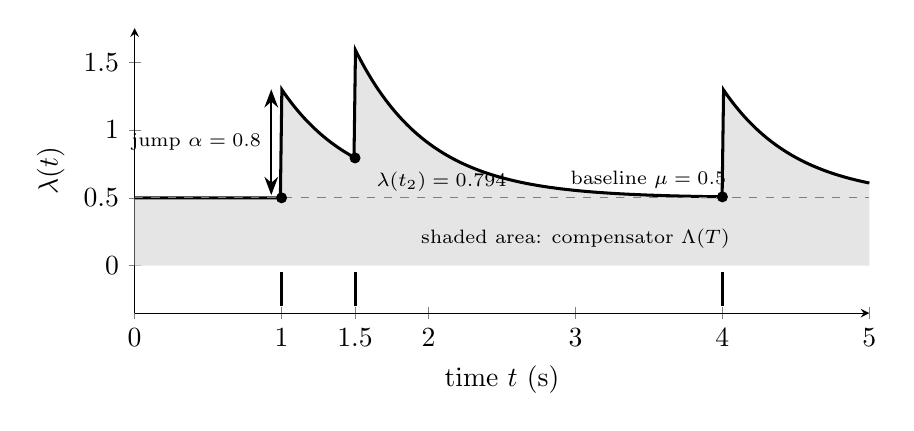
\begin{tikzpicture}
\begin{axis}[width=0.9\linewidth,height=5.2cm,xmin=0,xmax=5,ymin=-0.35,ymax=1.75,
  axis lines=left,xlabel={time $t$ (s)},ylabel={$\lambda(t)$},
  ytick={0,0.5,1,1.5},xtick={0,1,1.5,2,3,4,5},
  every axis plot/.append style={line width=1.1pt},clip=false]
  \addplot[name path=lam,color=black,samples=500,domain=0:5]
    {0.5+(x>1)*0.8*exp(-2*max(x-1,0))+(x>1.5)*0.8*exp(-2*max(x-1.5,0))+(x>4)*0.8*exp(-2*max(x-4,0))};
  \addplot[name path=zero,draw=none,domain=0:5]{0};
  \addplot[gray!20] fill between[of=lam and zero];
  \addplot[gray,dashed,thin,domain=0:5]{0.5};
  \node[font=\scriptsize,anchor=south west] at (axis cs:2.9,0.5) {baseline $\mu=0.5$};
  \foreach \t/\l in {1/0.5,1.5/0.794,4/0.507}{
    \edef\temp{\noexpand\draw[line width=1.1pt] (axis cs:\t,-0.3) -- (axis cs:\t,-0.05);
      \noexpand\fill (axis cs:\t,\l) circle (2pt);}
    \temp}
  \node[font=\scriptsize,anchor=north west] at (axis cs:1.58,0.76) {$\lambda(t_2)=0.794$};
  \draw[{Stealth}-{Stealth},thick] (axis cs:0.93,1.30) -- node[left,font=\scriptsize]{jump $\alpha=0.8$} (axis cs:0.93,0.52);
  \node[font=\scriptsize,align=center] at (axis cs:3.0,0.2) {shaded area: compensator $\Lambda(T)$};
\end{axis}
\end{tikzpicture}
\caption{Intensity of a univariate Hawkes process with \(\mu=0.5\), \(\alpha=0.8\) and
\(\beta=2\), for three events (ticks on the axis). Each event adds a jump that decays with
half-life \(\ln 2/2\approx0.35\)~s. The dots are the intensities at the events, the terms
that the likelihood rewards; the shaded area is the compensator, the term it penalizes.}
\label{fig:intensity}
\end{figure}

\paragraph{The intensity as a state.} Write \(E(t)=\lambda(t)-\mu\) for the excitation.
Between events, \(E\) decays as \(\mathrm dE/\mathrm dt=-\beta E\); at an event it jumps by
\(\alpha\). Hence, with \(\Delta_k=t_k-t_{k-1}\),
\begin{equation}
  E(t_k^-)=e^{-\beta\Delta_k}\bigl(E(t_{k-1}^-)+\alpha\bigr),
  \label{eq:recursion}
\end{equation}
and the current intensity summarizes the whole past: with an exponential kernel the
process \(\lambda(t)\) is Markov. This property makes simulation and the likelihood linear
in the number of events. It does not hold for other kernels, such as the power law, where
the whole history must be kept.

\paragraph{Cluster representation.} The same process can be generated as a population
\citep{hawkes2018,laub2021}. Immigrants arrive as a Poisson process of rate \(\mu\); each
event, immigrant or not, produces children as an inhomogeneous Poisson process of rate
\(\alpha e^{-\beta s}\), where \(s\) is the time since the parent. The number of direct
children of an event is Poisson with mean
\[
  g=\int_0^\infty\alpha e^{-\beta s}\,\mathrm ds=\frac{\alpha}{\beta},
\]
which is why \(g\) is called the branching ratio. Children, grandchildren and further
generations form a geometric series, so the mean size of the cluster started by one
immigrant is
\[
  1+g+g^2+\cdots=\frac{1}{1-g}\qquad(g<1),
\]
and a fraction \(g\) of all events is endogenous, triggered by earlier events rather than by
the baseline. Taking expectations in Equation~\eqref{eq:hawkes1d}, the stationary mean rate
\(\bar\lambda=\E[\lambda(t)]\) satisfies \(\bar\lambda=\mu+g\bar\lambda\), that is,
\(\bar\lambda=\mu/(1-g)\). Only the times are observed; the genealogy
(Figure~\ref{fig:cluster}) is latent.

\begin{figure}[htbp]
\centering
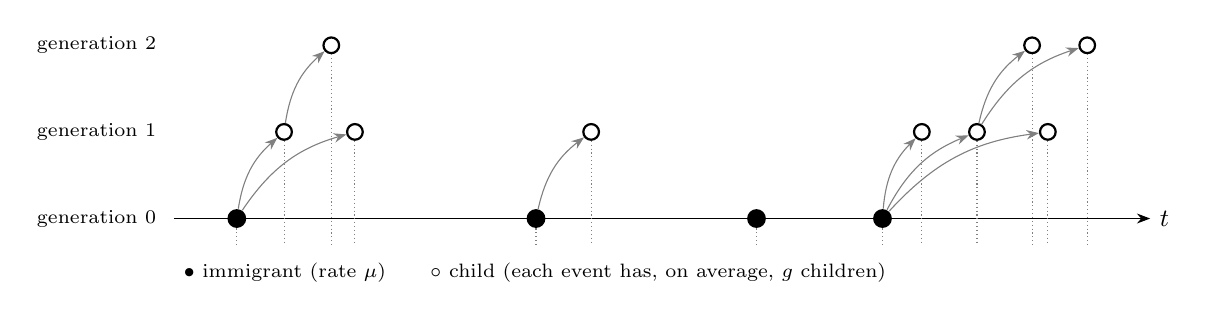
\begin{tikzpicture}[x=1.0cm,y=1.1cm,
  imig/.style={circle,fill=black,inner sep=2.4pt},
  child/.style={circle,draw=black,fill=white,thick,inner sep=2pt},
  link/.style={-{Stealth[length=1.6mm]},gray,thin}]
  \draw[-{Stealth}] (0,0) -- (12.4,0) node[right,font=\small]{$t$};
  \node[imig] (a) at (0.8,0) {};
  \node[child] (a1) at (1.4,1) {}; \node[child] (a2) at (2.3,1) {};
  \node[child] (a11) at (2.0,2) {};
  \draw[link] (a) to[bend left=20] (a1); \draw[link] (a) to[bend left=20] (a2);
  \draw[link] (a1) to[bend left=20] (a11);
  \node[imig] (b) at (4.6,0) {};
  \node[child] (b1) at (5.3,1) {};
  \draw[link] (b) to[bend left=20] (b1);
  \node[imig] (c) at (7.4,0) {};
  \node[imig] (d) at (9.0,0) {};
  \node[child] (d1) at (9.5,1) {}; \node[child] (d2) at (10.2,1) {}; \node[child] (d3) at (11.1,1) {};
  \node[child] (d21) at (10.9,2) {}; \node[child] (d22) at (11.6,2) {};
  \draw[link] (d) to[bend left=20] (d1); \draw[link] (d) to[bend left=20] (d2); \draw[link] (d) to[bend left=20] (d3);
  \draw[link] (d2) to[bend left=20] (d21); \draw[link] (d2) to[bend left=20] (d22);
  \foreach \p in {a,a1,a2,a11,b,b1,c,d,d1,d2,d3,d21,d22}{\draw[densely dotted,gray] (\p) -- (\p|-{(0,-0.3)});}
  \foreach \y in {0,1,2}{\node[font=\scriptsize,anchor=east] at (-0.1,\y) {generation \y};}
  \node[font=\scriptsize,anchor=north west] at (0,-0.4) {$\bullet$ immigrant (rate $\mu$)\qquad
    $\circ$ child (each event has, on average, $g$ children)};
\end{tikzpicture}
\caption{Cluster representation of a Hawkes process. Only the projection of the events on
the time axis is observed; which event triggered which is hidden. With \(g=0.5\), each
immigrant brings on average a cluster of \(1/(1-0.5)=2\) events.}
\label{fig:cluster}
\end{figure}

\section{Symmetric bivariate Hawkes process}

A \(D\)-dimensional Hawkes process has one intensity per type,
\[
 \lambda_i(t)=\mu_i+\sum_{j=1}^{D}\int_{(0,t)}\phi_{ij}(t-s)\,\mathrm dN_j(s),
 \qquad i=1,\dots,D,
\]
where \(\phi_{ij}\) is the effect of a type-\(j\) event on the intensity of type \(i\)
\citep{hawkes1971b,bacry2015}. With exponential kernels and two types there are, in general,
two baselines, four jump sizes and up to four decay rates. Here,
up-moves and down-moves are processes \(N_1,N_2\) with a common decay and symmetric
excitation:
\begin{align}
\lambda_1(t)&=\mu+\sum_{t_k^1<t}\alpha_{\mathrm{self}}e^{-\beta(t-t_k^1)}
 +\sum_{t_k^2<t}\alpha_{\mathrm{cross}}e^{-\beta(t-t_k^2)},\\
\lambda_2(t)&=\mu+\sum_{t_k^2<t}\alpha_{\mathrm{self}}e^{-\beta(t-t_k^2)}
 +\sum_{t_k^1<t}\alpha_{\mathrm{cross}}e^{-\beta(t-t_k^1)}.
\end{align}
The model reduces a general matrix to four parameters. This parsimony makes
simulation and comparison with \citet{lee2023} easier. Figure~\ref{fig:bivariate} draws it
as a diagram of the two event types. An up-move raises the intensity of another up-move by
\(\alpha_{\mathrm{self}}\) and that of a down-move by \(\alpha_{\mathrm{cross}}\), and
symmetrically for a down-move; both increases decay at the same rate \(\beta\). In
microstructure, dominant cross-excitation indicates reversion (an up-move followed by a
down-move), and dominant self-excitation indicates persistence of direction
\citep{bacry2013}.

\begin{figure}[htbp]
\centering
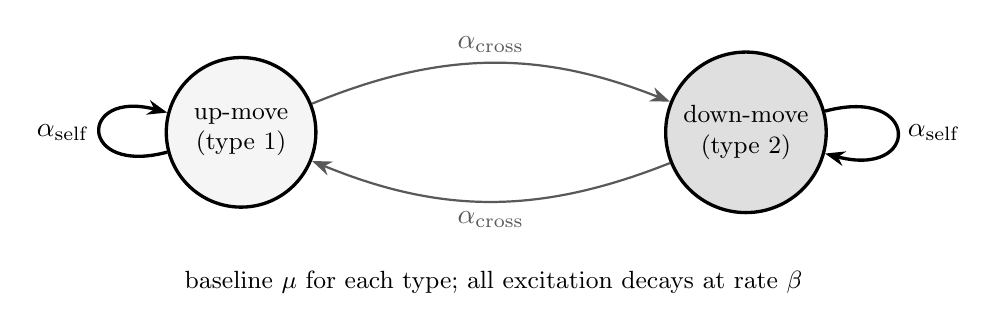
\begin{tikzpicture}[node distance=4.4cm,
  ev/.style={circle,draw=black,very thick,minimum size=1.9cm,font=\small,align=center}]
  \node[ev,fill=gray!8] (u) {up-move\\(type 1)};
  \node[ev,fill=gray!25,right=of u] (d) {down-move\\(type 2)};
  \draw[-{Stealth[length=2.5mm]},very thick] (u) edge[loop left,looseness=6]
    node[left]{$\alpha_{\mathrm{self}}$} (u);
  \draw[-{Stealth[length=2.5mm]},very thick] (d) edge[loop right,looseness=6]
    node[right]{$\alpha_{\mathrm{self}}$} (d);
  \draw[-{Stealth[length=2.5mm]},thick,gray!70!black] (u) to[bend left=22]
    node[above]{$\alpha_{\mathrm{cross}}$} (d);
  \draw[-{Stealth[length=2.5mm]},thick,gray!70!black] (d) to[bend left=22]
    node[below]{$\alpha_{\mathrm{cross}}$} (u);
  \node[font=\small] at ($(u)!0.5!(d)+(0,-1.9)$) {baseline $\mu$ for each type; all excitation decays at rate $\beta$};
\end{tikzpicture}
\caption{The symmetric bivariate Hawkes process as a diagram of event types. Loops are
self-excitation, arrows between types are cross-excitation; the same four parameters
\((\mu,\alpha_{\mathrm{self}},\alpha_{\mathrm{cross}},\beta)\) apply to both types.
\(\alpha_{\mathrm{self}}>\alpha_{\mathrm{cross}}\) describes persistence of direction, as
found in the crypto data of this work; \(\alpha_{\mathrm{cross}}>\alpha_{\mathrm{self}}\)
describes reversion, as at the equity fixed point of \citet{lee2023}.}
\label{fig:bivariate}
\end{figure}

\section{Stability}

The mass matrix of the kernels is
\[
 \mathbf G=\frac{1}{\beta}
 \begin{bmatrix}
  \alpha_{\mathrm{self}} & \alpha_{\mathrm{cross}}\\
  \alpha_{\mathrm{cross}} & \alpha_{\mathrm{self}}
 \end{bmatrix}.
\]
Its entry \((i,j)\) is the mean number of type-\(i\) children of a type-\(j\) event, so
\(\mathbf G\) plays the role of the branching ratio. Its eigenvalues are
\((\alpha_{\mathrm{self}}-\alpha_{\mathrm{cross}})/\beta\) and the largest,
\[
 g=\frac{\alpha_{\mathrm{self}}+\alpha_{\mathrm{cross}}}{\beta},
\]
which is the mean number of children of either type per event. The two eigenvalues have
eigenvectors \((1,1)\) and \((1,-1)\): the first governs the total activity
\(N_1+N_2\), the second the difference \(N_1-N_2\), that is, the price
(Section~\ref{sec:volatility-theory}). Write
\[
 g_-=\frac{\alpha_{\mathrm{self}}-\alpha_{\mathrm{cross}}}{\beta}
\]
for the second eigenvalue. The condition \(g<1\) is
required. Close to one, cascades last longer; above one, there is no usual stationary
regime \citep{hardiman2013,filimonov2012}. Under stationarity, by the same argument as in
the univariate case, each type occurs at mean rate \(\mu/(1-g)\), and the two together at
\(2\mu/(1-g)\).

\section{Marks and price}

An event has a time, a type and a mark. The mark is the size of the change in ticks.
The paper keeps the mark for volatility, but assumes that the intensity does not
depend on it. The filtered price can be written, in ticks, as the cumulative
difference between up-moves and down-moves.

\section{Volatility}
\label{sec:volatility-theory}

In a minimal model, if the price moves by one tick \(\vartheta\) at a rate \(\phi\),
\[
 \sigma^2\approx\phi\vartheta^2.
\]
Thus, modeling intensity is modeling activity and, consequently, a component of
volatility. The marked Hawkes expression requires moments of the marks and the
estimated parameters \citep{leeseo2017,lee2024}.

\paragraph{Long-run variance of the Hawkes price.} With unit marks the price is
\(X(t)=N_1(t)-N_2(t)\), the projection on the eigenvector \((1,-1)\). Under stationarity each
type has mean rate \(\bar\lambda=\mu/(1-g)\), and the variance of \(X\) per unit time
converges, as the horizon grows, to
\[
 \lim_{T\to\infty}\frac{\Var X(T)}{T}=\frac{2\bar\lambda}{(1-g_-)^2}
\]
\citep{bacry2013}. If each event moves the price by an i.i.d.\ size \(J\), independent of the
times, with the sign given by the type, the same argument gives
\begin{equation}
 \sigma_H^2=2\bar\lambda\left[\Var(J)+\frac{\E[J]^2}{(1-g_-)^2}\right],
 \label{eq:hawkes-variance}
\end{equation}
the expression used in Section~\ref{sec:real-volatility}. The total activity depends on
\(g\), and the amplification of the variance on \(g_-\). When self-excitation dominates,
\(g_->0\) and moves in the same direction cluster, so the variance exceeds that of a Poisson
price with the same activity. When cross-excitation dominates, \(g_-<0\), moves tend to undo
each other and the variance falls below it; this is the mechanism that \citet{bacry2013} use
to model microstructure noise. When \(\alpha_{\mathrm{self}}=\alpha_{\mathrm{cross}}\), the
long-run variance equals that of the difference of two independent Poisson processes with the
same activity.

\paragraph{Realized volatility.} The benchmark is the realized variance over a window,
\[
 \mathrm{RV}_\Delta=\sum_k r_k^2,
\]
the sum of squared log returns sampled every \(\Delta\) seconds
\citep{andersen2003,barndorff2002}. Without noise, it converges to the integrated variance as
\(\Delta\to0\). At high frequency, however, the observed price contains microstructure noise,
and \(\mathrm{RV}_\Delta\) is biased upward when \(\Delta\) is small \citep{zhang2005}. The
signature plot, \(\mathrm{RV}_\Delta\) per unit time against \(\Delta\), shows the effect:
noise makes it fall with \(\Delta\), while positively autocorrelated returns, as in a
self-exciting price, make it rise toward the long-run level of
Equation~\eqref{eq:hawkes-variance}.

\section{Simulation}

A Hawkes path can be simulated by Ogata's thinning \citep{ogata1981}. If
\(\lambda(t)\le M\) on an interval, candidates are drawn from a Poisson process of rate
\(M\) and each candidate at time \(s\) is kept with probability \(\lambda(s)/M\); the kept
points have intensity \(\lambda\). With an exponential kernel the intensity only decreases
between events, so its value just after the last event is a valid bound until the next
event. In the bivariate case the bound is \(\lambda_1+\lambda_2\), and the type of an
accepted event is drawn in proportion to \(\lambda_1\) and \(\lambda_2\). The
implementation is described in Section~\ref{sec:sim-thinning}.

\section{Maximum likelihood}
\label{sec:mle-theory}

For a horizon \(T\),
\[
 \ell(\theta)=\sum_k\log\lambda_{c_k}(t_k)
 -\sum_i\int_0^T\lambda_i(u)\,du.
\]
The first term rewards high intensity at the events; the second penalizes high
intensity over the whole interval. Maximizing only the first would drive the
intensities to infinity. The compensator provides the balance. For an exponential
kernel, the sum over the past obeys a first-order recursion, and \(\ell\) and its
gradient can be computed in \(O(n)\) operations \citep{ozaki1979}. In the univariate case,
let \(A_1=0\) and \(A_k=e^{-\beta(t_k-t_{k-1})}(1+A_{k-1})\), so that \(\alpha A_k\) is
the excitation just before \(t_k\) (Equation~\eqref{eq:recursion}). Then
\begin{equation}
 \ell(\mu,\alpha,\beta)=\sum_{k=1}^{n}\log\bigl(\mu+\alpha A_k\bigr)-\mu T
 -\frac{\alpha}{\beta}\sum_{k=1}^{n}\Bigl(1-e^{-\beta(T-t_k)}\Bigr).
 \label{eq:loglik1d}
\end{equation}
The bivariate likelihood has the same structure, with one recursion per pair of source and
target types. Under regularity conditions, the MLE is consistent and asymptotically
efficient \citep{ogata1978}: approximately normal around the true value, with covariance
given by the inverse Fisher information, which the inverse of the observed Hessian of
\(-\ell\) estimates. These conditions include a true parameter in the interior of the
parameter space. When it lies on the boundary, as \(\alpha_{\mathrm{cross}}=0\), the
estimate piles up at the boundary with positive probability, and neither the normal
approximation nor the usual \(\chi^2\) reference for likelihood ratio tests applies
\citep{selfliang1987}. This is relevant for the real data of this work, where
\(\alpha_{\mathrm{cross}}\) is estimated close to zero.

\section{Model comparison}

The Poisson process is nested in the Hawkes process: it is the case
\(\alpha_{\mathrm{self}}=\alpha_{\mathrm{cross}}=0\). The likelihood ratio statistic
\(2(\hat\ell_{\mathrm{Hawkes}}-\hat\ell_{\mathrm{Poisson}})\) measures the gain in fit. Its
usual \(\chi^2\) reference does not hold here for two reasons: the null value lies on the
boundary of the parameter space \citep{selfliang1987}, and \(\beta\) has no effect under the
null, so it is not identified there. The Akaike information criterion,
\[
 \mathrm{AIC}=2k-2\hat\ell,
\]
with \(k\) the number of free parameters, compares the two fits with a penalty for the extra
parameters \citep{akaike1974}. A difference in AIC of hundreds of units, as found on the real
windows, leaves no doubt about the direction, whatever the exact reference distribution.

\section{Goodness of fit by time rescaling}
\label{sec:time-rescaling}

If the model is correct, the compensator turns the observed process into a unit-rate
Poisson process: the transformed times \(\Lambda(t_k)\) are the events of a homogeneous
Poisson process of rate one. This is the time-rescaling theorem \citep{brown2002}. The
increments
\[
 \tau_k=\Lambda(t_k)-\Lambda(t_{k-1})=\int_{t_{k-1}}^{t_k}\lambda(u)\,\mathrm du
\]
are then independent \(\mathrm{Exp}(1)\) variables. In the bivariate case the theorem
applies to each type with its own compensator \(\Lambda_i\). Evaluated at the estimated
parameters, the \(\tau_k\) are the rescaled residuals of the fit \citep{ogata1988}. Their
distribution is tested against \(\mathrm{Exp}(1)\), for example with Kolmogorov--Smirnov,
and their serial dependence with Ljung--Box. A kernel of the wrong shape typically leaves
dependence in the residuals: bursts that the fitted kernel forgets too fast or too slowly
appear as runs of short or long \(\tau_k\).

\section{Observation on a time grid}

The events of this work are changes of the mid-price recorded on a 100~ms grid
(Chapter~\ref{cap:dados}). Two things are lost relative to continuous time: event times are
rounded to the grid, and changes that fall in the same cell merge into one. The second
matters most for the decay. With \(\beta\) of a few units per second, much of the excitation
acts within a few hundred milliseconds, and merged events remove part of the short
inter-arrivals from which \(\beta\) is identified. A likelihood written for continuous time
therefore estimates the parameters of the process as seen through the grid, with \(\beta\)
biased downward; Section~\ref{sec:addendum-grid} measures the size of this bias.
Likelihoods that account for the observation scheme have been proposed for this setting
\citep{lambe2025}.

A biased estimator can still be corrected by simulation, the idea of indirect inference
\citep{gourieroux1993}. Let \(b(\theta)\) be a summary, such as the median, of the grid MLE
over paths simulated from \(\theta\) in continuous time and mapped to the grid. The map
\(b\) is estimated by simulation, and an estimate on the grid is corrected by solving
\(b(\theta)=\hat\theta_{\mathrm{grid}}\). The correction is as good as the model used to
simulate: if the real process is not a Hawkes process, the map transfers its bias with it.
A network trained on gridded paths with the continuous-time parameter as target learns a
correction of the same kind, conditional on the whole path.

\section{Identifiability in finite samples}
\label{sec:identificabilidade}

The asymptotic properties do not guarantee good behavior with 1,000 events. When the
excitation is weak (small \(\alpha_{\mathrm{self}}+\alpha_{\mathrm{cross}}\)), the
kernel barely changes the intensity, and the likelihood becomes flat in the direction
of \(\beta\): very different values of \(\beta\) explain the data almost equally well.
In the limit \(\alpha\to0\), \(\beta\) is no longer identified. Near criticality, the
separation between \(\mu\) and \(g\) also deteriorates, because the mean rate
\(2\mu/(1-g)\) is well determined, but neither factor is on its own. These effects
reappear in the results of Chapter~\ref{cap:resultados}.

\section{Amortized estimation as a Bayes estimator}
\label{sec:bayes}

In the approach of \citet{lee2023}, a network \(f_\phi\) is trained on pairs
\((\theta_i,x_i)\), where \(\theta_i\) is drawn from a training distribution \(\pi\)
and \(x_i\) is simulated from the model with parameter \(\theta_i\). Minimizing the
mean squared error,
\[
  \min_\phi\;\E_{\theta\sim\pi}\,\E_{x\mid\theta}
  \bigl\lVert f_\phi(x)-\theta\bigr\rVert^2,
\]
is minimizing the Bayes risk under squared loss, whose solution is the posterior mean
\(\E_\pi[\theta\mid x]\) \citep{lehmann1998}. Hence, a well-trained network
approximates a Bayes estimator under the prior \(\pi\)
\citep{sainsburydale2024,lenzi2023}. Two consequences guide this work. First, on a
test set drawn from the same \(\pi\), no estimator has lower average MSE than the
posterior mean, so outperforming the MLE on that test is expected and does not prove
superiority in a frequentist sense. Second, the network does not extrapolate: its
estimates shrink toward the high-density region of \(\pi\), and real data outside the
support of the prior yield biased estimates.

The same approach belongs to a wider family of amortized, simulation-based inference methods,
in which the cost of inference is paid once, in training, and each new data set costs a
forward pass \citep{cranmer2020,radev2022}. On real windows the target changes. When a
network is trained on pairs \((x,\hat\theta_{\mathrm{MLE}}(x))\), the label is a deterministic
function of the input, so the minimizer of the squared loss is the MLE itself: the network
becomes a fast approximation of the MLE map, accurate where the training windows are dense.
Starting from the weights trained on simulated data, it can reach that approximation with
fewer real windows; how close the simulation prior is to the real data then matters for how
much that initialization helps.

\section{Comparing estimators}
\label{sec:comparing-theory}

The estimators are compared path by path. For each path or window \(i\), a loss
\(L_i(A)\), such as the squared error averaged over the four parameters, is computed for each
estimator \(A\); the macro MSE is the average of the per-parameter MSEs. Two estimators are
compared through the paired differences \(d_i=L_i(A)-L_i(B)\). Pairing removes the variation
in difficulty between paths, which is often much larger than the difference between
estimators.
The mean \(\bar d\) is reported with a bootstrap confidence interval, obtained by resampling
the \(d_i\) with replacement \citep{efron1993}, and the null hypothesis of no difference is
tested with the Wilcoxon signed-rank test, which uses the ranks of \(|d_i|\) and is robust to
the heavy tails of squared errors \citep{wilcoxon1945,diebold1995}. Variation across training
seeds is a different source: it measures the instability of training, not the accuracy of a
trained model, and is compared across seeds \citep{bouthillier2021}.

When several comparisons are tested together, the Holm procedure controls the probability
of any false rejection: with the \(m\) \(p\)-values sorted in increasing order, the \(k\)-th
is compared with \(0.05/(m-k+1)\), and testing stops at the first non-rejection
\citep{holm1979}. Agreement between two orderings, such as the Hawkes and the realized
volatilities across windows, is measured by the Spearman correlation, the correlation of the
ranks, which ignores the level and depends only on the order.

\paragraph{Ensembles.} The average \(\bar y=\frac1M\sum_m y_m\) of \(M\) estimators satisfies
\[
 \lVert\bar y-\theta\rVert^2=\frac1M\sum_{m=1}^{M}\lVert y_m-\theta\rVert^2
 -\frac1M\sum_{m=1}^{M}\lVert y_m-\bar y\rVert^2
\]
\citep{krogh1995}. The error of the average equals the average error of the members minus
their spread, so it is never worse than the average member, and it improves most when the
members are accurate and err in different places. This identity applies both to the
ensembles of five seeds and to the average of the LSTM and the Transformer.

\section{LSTM}

Recurrent networks update a state \(h_t=f(x_t,h_{t-1})\). The LSTM introduces input,
forget and output gates to control the flow of information and mitigate the
vanishing gradient problem \citep{hochreiter1997}. With \(\sigma\) the logistic function
and \(\odot\) the elementwise product,
\begin{align*}
 f_t&=\sigma(W_f[h_{t-1},x_t]+b_f), & i_t&=\sigma(W_i[h_{t-1},x_t]+b_i),\\
 o_t&=\sigma(W_o[h_{t-1},x_t]+b_o), & \tilde c_t&=\tanh(W_c[h_{t-1},x_t]+b_c),\\
 c_t&=f_t\odot c_{t-1}+i_t\odot\tilde c_t, & h_t&=o_t\odot\tanh(c_t).
\end{align*}
The cell state \(c_t\) is updated additively, which lets gradients pass over many steps.
The update has the form of Equation~\eqref{eq:recursion}: a forget gate that depends on the
inter-arrival time can play the role of \(e^{-\beta\Delta_k}\), and the input gate that of
the jump, so an LSTM can represent the excitation of a Hawkes process in its state. In
Lee, the sequence contains the inter-arrival time and the type; the final state feeds the
regression of the four parameters. The paper also tested a GRU \citep{cho2014}, with
slightly worse results.

\section{Attention and the Transformer}

Attention computes weighted combinations:
\[
 \operatorname{Attention}(Q,K,V)=
 \operatorname{softmax}\left(\frac{QK^\top}{\sqrt{d_k}}\right)V.
\]
Each position queries all the others. The Transformer combines multiple heads,
feed-forward layers, residual connections and normalization \citep{vaswani2017}. Each head
applies its own projections \(Q=XW^Q\), \(K=XW^K\), \(V=XW^V\) to the sequence \(X\), and
the heads are concatenated. Self-attention is equivariant to permutations of the sequence,
so order and spacing must enter through a positional encoding; for a point process the
relevant position is the time of each event, not only its index. The
potential advantage is capturing distant dependencies; the potential cost is
\(O(n^2)\) memory. The position of the normalization relative to the residual
connections affects training stability: the \emph{post-LN} variant, used here,
usually requires learning-rate warm-up \citep{xiong2020}.

\section{Training}

The networks are trained by stochastic gradient descent on mini-batches with Adam, which
scales each step by running estimates of the first and second moments of the gradient
\citep{kingma2015}. The learning rate can follow a schedule, such as a short warm-up or a cosine decay
\citep{xiong2020,loshchilov2017}. Training stops at a fixed budget of epochs or when the
validation loss stops improving, and the checkpoint with the lowest validation loss is kept;
the test data are not used for any choice. Fine-tuning reuses this procedure from weights
already trained on another task, here the simulated paths, with the real windows as the new
training set.

\chapter{Related Work}

\section{Hawkes processes in finance}

After the original formulation \citep{hawkes1971,hawkes1971b}, self- and mutually
exciting models came to describe market events in continuous time
\citep{bowsher2007,embrechts2011}, contagion between markets \citep{aitsahalia2015}
and endogeneity, measured by the branching ratio \citep{filimonov2012,hardiman2013}.
\citet{bacry2013} use a bivariate Hawkes process of up- and down-moves to reproduce
the microstructure noise of the price; cross-excitation captures reversion at short
scales. \citet{bacry2015} and \citet{hawkes2018} review this field, and
\citet{mutoke2011} offers a didactic introduction. \citet{leeseo2017} connect the
marked Hawkes process to the price in ticks and derive Hawkes volatility, which
\citet{lee2024} apply to filtered prices. In Brazil, \citet{primo2018} analyzes the
intraday clustering of stocks with MLE, and \citet{silva2026} systematizes inference,
diagnostics and financial applications.

\section{Estimation of Hawkes processes}

MLE for exponential kernels dates back to \citet{ozaki1979}, with asymptotic
properties established by \citet{ogata1978}. Simulation by \emph{thinning}
\citep{ogata1981} and diagnostics by rescaled residuals \citep{ogata1988,brown2002}
complete the classical toolbox \citep{laub2021}. The optimization is sensitive to the
initialization and to the geometry of the likelihood, which can be nearly flat in
some directions when the series is short (Section~\ref{sec:identificabilidade}).

\section{Amortized and simulation-based inference}

When the likelihood is expensive or intractable, networks trained on simulations
replace the optimization with a single forward pass \citep{cranmer2020}. Networks
trained on simulations already estimate parameters of spatial and extreme-value
models \citep{gerber2021,lenzi2023}; with squared loss, they approximate Bayes
estimators \citep{sainsburydale2024}, and methods such as BayesFlow learn the full
posterior \citep{radev2022}. \citet{lee2023} applies the idea to the 2D Hawkes process
with an LSTM. \citet{lambe2025} use networks for the Hawkes process observed only
through interval counts, a case in which the exact likelihood is intractable and the
MLE is no longer a direct alternative.

\section{Neural point processes}

Another line of work uses networks to model the intensity itself, without the
parametric form of Hawkes: RMTPP \citep{du2016}, the Neural Hawkes Process
\citep{mei2017} and attention-based variants such as the Transformer Hawkes Process
\citep{zuo2020} and the Self-Attentive Hawkes Process \citep{zhang2020};
\citet{shchur2021} review the area. The goal differs from that of this work: those
models maximize predictive likelihood, whereas here the network estimates the four
interpretable parameters of a classical model.

\section{Hawkes processes in crypto-assets}

Using one-minute returns of 17 cryptocurrencies traded on Binance,
\citet{taddeo2024} show that Hawkes describes the occurrence of jumps in log-returns
better than Poisson. The crypto market also exhibits segmentation and limited
arbitrage across exchanges \citep{makarov2020}, and perpetual futures, which have no
expiry and carry a funding rate, concentrate a large share of the liquidity
\citep{he2022perpetual}.

\section{Positioning}

\begin{table}[htbp]
\centering
\caption{Positioning of this work relative to the closely related literature.}
\label{tab:posicionamento}
\small
\begin{tabularx}{\linewidth}{lllX}
\toprule
Work & Estimation & Architecture & Market\\
\midrule
\citet{bacry2013} & MLE & -- & futures (Bund, DAX)\\
\citet{leeseo2017} & MLE & -- & equities\\
\citet{primo2018} & MLE & -- & equities (Brazil)\\
\citet{taddeo2024} & MLE & -- & crypto (jumps in 1-min returns)\\
\citet{lee2023} & network & LSTM & equities (US)\\
\citet{lambe2025} & network & MLP & synthetic (counts)\\
\citet{zuo2020} & neural intensity & Transformer & generic\\
This work & network and MLE & LSTM and Transformer & crypto (perpetual futures)\\
\bottomrule
\end{tabularx}
\end{table}

The present work combines controlled reproduction, public crypto data and a
comparison with attention, and adds to the evaluation of \citet{lee2023} robust
metrics, paired tests and the interpretation of the network as a Bayes estimator.

\chapter{Data}
\label{cap:dados}

\section{Source and market}

Both spot and futures were evaluated. The need for the best bid/ask ruled out the
official spot archive, which has no equivalent historical \dataset{bookTicker}. USD-M
futures provide \dataset{bookTicker} and \dataset{aggTrades}. The symbols are BTCUSDT
and ETHUSDT \citep{binancePublicData}.

\section{Schema}

\dataset{bookTicker} includes an identifier, the best bid and ask prices and
quantities, the transaction time and the event time. The canonical schema has a UTC
timestamp, bid, ask and quantities. Audits check for positive prices, bid less than
or equal to ask, ordering and temporal duplicates.

\section{Sampling}

Updates can occur every millisecond, a much finer resolution than the chosen scale.
Timestamps are grouped into 100 ms bins and the last state is kept. This filter
follows Lee's protocol and reduces ultra-high-frequency noise.

\section{Datasets produced}

\begin{table}[htbp]
\centering
\caption{Dataset coverage.}
\label{tab:cobertura}
\begin{tabular}{lrrr}
\toprule
Window & Symbol-days & Events & Segments of 1,000\\
\midrule
Primary (Jan.\ 2024) & 28 & 1,826,904 & 1,813\\
Robustness (Oct.\ 2023) & 14 & 1,288,352 & 1,281\\
\bottomrule
\end{tabular}
\end{table}

\section{Event characteristics}
\label{sec:caracteristicas}

Table~\ref{tab:caracteristicas} summarizes the events of the calibration block
(January 15 to 22, 2024). Three facts distinguish these data from the setting of
\citet{lee2023}. First, about 76\% of the changes repeat the direction of the previous
one, which indicates persistence rather than reversion. Second, the median jump is 10
to 15 ticks and only 10--13\% of the jumps are one tick: at the 100~ms scale, these
contracts behave as small-tick assets. Third, 37--39\% of the inter-arrival times are
exactly 0.1~s, the grid step; the sampling strongly discretizes the times, whereas the
model and the simulations assume continuous time.

\begin{table}[htbp]
\centering
\caption{Characteristics of the mid-price events, January 15 to 22, 2024.}
\label{tab:caracteristicas}
\small
\begin{tabular}{lrr}
\toprule
 & BTCUSDT & ETHUSDT\\
\midrule
Events & 529,278 & 540,164\\
Fraction of up-moves & 49.4\% & 49.5\%\\
Probability of repeating the previous direction & 76.0\% & 75.7\%\\
Median inter-arrival time & 0.3 s & 0.3 s\\
Inter-arrival times equal to 0.1 s (grid) & 39.5\% & 37.3\%\\
Median / 90th percentile jump (ticks) & 15.5 / 48 & 10 / 29\\
One-tick jumps & 9.7\% & 12.6\%\\
\bottomrule
\end{tabular}
\end{table}

\chapter{Methodology}

\section{Principles}

The protocol distinguishes:
\begin{description}
  \item[R1:] explicitly published information;
  \item[R2:] reconstruction to fill a gap;
  \item[A1:] adaptation required for crypto;
  \item[E1:] extension with a Transformer.
\end{description}

\section{Pipeline}

\begin{enumerate}
  \item build the daily URL and download the ZIP;
  \item compute the SHA-256 and record it in a manifest;
  \item temporarily extract the CSV;
  \item process chunks of one million rows;
  \item reduce the updates to the 100 ms grid;
  \item produce Parquet partitioned by symbol and date;
  \item delete the temporary CSV;
  \item create windows without crossing splits;
  \item fit the MLE and calibrate ranges on the training set only;
  \item generate synthetic paths and train the estimators;
  \item select hyperparameters on the validation set;
  \item open the test set only once.
\end{enumerate}

\section{Simulation by thinning}
\label{sec:sim-thinning}

Given the current state, an upper bound on the sum of the intensities is computed. An
exponential waiting time is drawn; the excitation decays; the candidate is accepted
with probability proportional to the new intensity \citep{ogata1981}. The type is
drawn with probabilities proportional to \(\lambda_1,\lambda_2\). After the event, the
corresponding column of the \(\alpha\) matrix is added. Each path starts with an
empty history, the same assumption as in the likelihood.

\section{Constrained MLE}

Positive parameters are obtained through softplus. Instead of optimizing \(\beta\)
freely, a positive margin \(d\) is used:
\[
(\mu,\alpha_s,\alpha_c,d)=\softplus(z),\qquad
\beta=\alpha_s+\alpha_c+d.
\]
L-BFGS-B is started from five points: one based on the empirical event rate and four
random perturbations in the unconstrained space. The MLE never receives the true
parameter as initialization. The gradient is analytic, and the exponential
recursions are solved as bidiagonal systems. Convergence, iterations, log-likelihood
and time are recorded.

\section{Neural protocol}

The target is \((\mu,\alpha_s,\alpha_c,\beta)\), and the loss is the MSE on the
original scale. The input for each event is \((\log(1+\Delta t),\,s)\), with \(s=+1\)
for an up-move and \(s=-1\) for a down-move; Lee uses inter-arrival times and types
1/2, so this transformation is a reconstruction (R2). The two networks share the
output head: softplus produces \(\mu,\alpha_s,\alpha_c,d>0\) and
\(\beta=\alpha_s+\alpha_c+d\), which guarantees \(g<1\) by construction, as in Lee's
robust version.

The frozen synthetic experiment contains 75,000 training sequences, 10,000 validation
sequences and 15,000 test sequences, all of exactly 1,000 events. The parameters are
drawn with \(\mu\in[0.2,\,0.6]\), \(\beta\in[0.8,\,2.0]\), self-excited fraction
\(\alpha_s/(\alpha_s+\alpha_c)\in[0.2,\,0.8]\) and \(g\) balanced across three
strata: low \([0.10,\,0.35)\), intermediate \([0.35,\,0.70)\) and near-critical
\([0.70,\,0.95]\). Table~\ref{tab:treino} summarizes the training.

\begin{table}[htbp]
\centering
\caption{Training configuration and cost (five seeds per network, Apple Silicon Mac
with MPS).}
\label{tab:treino}
\small
\begin{tabular}{lrr}
\toprule
 & LSTM (R1/R2) & Transformer (E1)\\
\midrule
Architecture & 2 LSTM $\times$ 12 + dense & encoder, 2 layers, $d=32$\\
Heads / feed-forward & -- & 4 / 128\\
Trainable parameters & 2,068 & 25,700\\
Optimizer & Adam, $10^{-3}$ & Adam, $10^{-3}$\\
Effective batch & 64 & 8 (physical 4 with accumulation)\\
Maximum epochs / patience & 300 / 30 & 300 / 30\\
Best epoch (per seed) & 165, 164, 193, 239, 299 & 73, 42, 38, 60, 44\\
Training time per seed & 5.4--14.8 h & 16.6--28.8 h\\
Total time (5 seeds) & 41 h & 110 h\\
\bottomrule
\end{tabular}
\end{table}

The Transformer's tensor flow starts from \([B,L,2]\), with \(L=1000\). A linear
projection produces \([B,L,32]\), to which the positional encoding is added. In each
layer, the four heads operate in subspaces of dimension eight; the feed-forward block
expands 32 to 128 and returns to 32. Temporal averaging converts \([B,L,32]\) into
\([B,32]\). The memory cost of attention grows quadratically with \(L\), which is why
its batch is smaller than the LSTM's. This difference in batch size, together with the
absence of a hyperparameter search for either network, is a limitation of the
comparison.

\section{The paper's fixed point (E2)}

To compare directly with the sampling-distribution table of \citet{lee2023}, 2,000
paths of 1,000 events were simulated at the published point
\((\mu,\alpha_s,\alpha_c,\beta)=(0.3,\,0.4,\,0.7,\,1.5)\), which lies inside the
training prior. The networks were applied without retraining, and the MLE was fitted
in two versions: the protocol's heuristic and the initialization at the true value
used in the paper.

\section{Empirical protocol}
\label{sec:empirical-protocol}

On real data there is no true parameter, so the empirical stage asks three narrower
questions: whether the Hawkes model describes the windows well enough to be estimated, whether
a network can reproduce the MLE on real windows, and whether the estimated parameters give a
volatility consistent with the realized one. The protocol was fixed in a decision record
(ADR~008) before the test block was opened. The windows have 1,000 events and are split
chronologically by day: calibration (15--22 January 2024, 1,063 windows), validation (23--25
January, 476 windows) and test (26--28 January, 274 windows); the October 2023 week is a
robustness window that is never used for training or selection.

\paragraph{Goodness of fit.} With the MLE of each calibration window, the time-rescaled
residuals of each dimension are tested against \(\mathrm{Exp}(1)\) with Kolmogorov--Smirnov and
for serial dependence with Ljung--Box at 10 lags \citep{ogata1988,brown2002}, and the Hawkes
model is compared with a homogeneous bivariate Poisson process by likelihood ratio and AIC.
Since the times lie on a 100~ms grid, two controls separate the effect of the grid from
misspecification: times jittered uniformly inside their cell with the MLE refitted, and paths
simulated from each fitted model, either in continuous time or mapped to the grid in the same
way as the data. The rejection rate of the simulated controls is what a correct model would
produce.

\paragraph{Networks on real windows.} Each window is labeled with its MLE (five heuristic
starts). Both architectures are trained on the calibration labels with the loss, batch size,
maximum of 300 epochs and patience of 30 of the synthetic protocol, in two variants: from
scratch (Adam, \(10^{-3}\)) and fine-tuned from the synthetic weights of the same seed (Adam,
\(10^{-4}\)), each with the five protocol seeds. Two references need no training: the synthetic
networks as they are, and the mean of the training labels, which is the best constant
predictor. The selected variant is the one whose five-seed ensemble has the lowest macro MSE
on validation. The test block is labeled and read once, after the selection; the stored
weights are evaluated without retraining, and every variant is reported. The machine budget
for this stage was capped at 30 hours.

\paragraph{Volatility.} The long-run volatility implied by the estimated parameters
(Section~\ref{sec:real-volatility}) is compared window by window with the realized volatility
of the log mid-price sampled every \(\Delta\in\{0.1, 1, 5, 10, 30\}\) seconds, using the median
ratio and the Spearman correlation across windows, with \(\Delta=10\)~s as the main horizon,
for the MLE and for the selected network.

\section{Metrics and tests}

The reported metrics are per-parameter and aggregate MSE, median absolute error,
bias, validity, branching-ratio error, cost and MLE convergence. Because the
parameters have different scales, the \(R^2\) of each parameter relative to the prior
mean (the trivial estimator) is also reported. The comparison between networks uses
two sources of variation: across seeds (Welch and Mann--Whitney tests with five
seeds), which measures training variability \citep{bouthillier2021}, and across test
paths (paired difference with a \emph{bootstrap} CI and Wilcoxon test), which measures
the accuracy of the already trained models \citep{efron1993,diebold1995}.

\chapter{Results}
\label{cap:resultados}

\section{Data gate}

All 56 primary files were present. Twenty-eight partitions were generated. BTCUSDT
produced 887,803 events; ETHUSDT, 939,101. The independent window produced 1,288,352
events. The availability and volume gate was therefore satisfied.

\section{Reproduction at the fixed point}

\input{en/e2_fixed_point.tex}

Table~\ref{tab:e2-ponto-fixo} reproduces the qualitative pattern of \citet{lee2023}.
The MLE is practically unbiased, and its standard deviations are about \(\sqrt{2}\)
times those in the paper, as expected for paths of half the length. The networks show
the characteristic shrinkage bias: they pull \(\alpha_{\mathrm{self}}\) and
\(\alpha_{\mathrm{cross}}\) toward the center of the prior, as in the paper, in
exchange for lower variance. The two versions of the MLE produced exactly the same
estimates, so the initialization at the true value used by Lee does not explain the
MLE's advantage at this well-identified point (\(g\approx0.73\)). The macro MSE was
0.0103 for the MLE and 0.0111 for the LSTM ensemble.

\section{Final comparison: LSTM, Transformer and MLE}

\input{en/final_results.tex}

\input{en/posthoc_results.tex}

\section{Computational cost}
\label{sec:custo}

The final run recorded 105~ms of wall-clock time per path for the MLE with four
processes. This value was measured while neural training was occupying the GPU. A
controlled benchmark on the same machine, with the same code (which exactly
reproduces the 15,000 recorded estimates), produced the values in
Table~\ref{tab:custo}.

\begin{table}[htbp]
\centering
\caption{Cost per path of 1,000 events in a controlled benchmark.}
\label{tab:custo}
\small
\begin{tabular}{lr}
\toprule
Estimator and execution mode & Time per path\\
\midrule
MLE, 5 starts, one core & 9.6 ms\\
MLE, 1 start, one core & 2.2 ms\\
MLE, 5 starts, 4 processes (wall-clock) & 2.5 ms\\
LSTM, batch size one, CPU (1 thread) / MPS & 7.0 ms / 29.6 ms\\
Transformer, batch size one, CPU (1 thread / 10 threads) / MPS & 9.9 / 4.8 / 5.0 ms\\
LSTM, batch of 256 on MPS & 0.07 ms\\
Transformer, batch of 32 on MPS & 3.7 ms\\
\midrule
\citet{lee2023}: network / MLE & 12 ms / 1,763 ms\\
\bottomrule
\end{tabular}
\end{table}

With an analytic gradient and a linear recursion, the MLE of this four-parameter
model costs a few milliseconds, the same order as neural inference at batch size one.
The ratio of about 150 times reported by Lee is not reproduced. The cost advantage of
the networks appears in batched inference, especially for the LSTM, and would grow
for models with more expensive likelihoods.

Lee does not describe the implementation of the MLE. To find where its 1,763~ms come from,
the same paths at Lee's fixed point were fitted with implementations that differ in one factor
at a time, at 1,000 and 2,000 events, the two lengths the paper mentions
(Appendix~\ref{ap:lee}). All variants reach the same estimates (largest difference 0.002 in any
parameter); only the cost changes (Table~\ref{tab:custo-variantes}). The likelihood is the
dominant factor: computed as a double sum over pairs of events, it costs about 90 times as much
as the recursion at 2,000 events, while a numerical gradient and a derivative-free optimizer
(Nelder--Mead) multiply the cost by about five each. With the recursion, even an interpreted
loop stays below 0.1~s, and the time reported by Lee falls between the two vectorized
double-sum variants at 2,000 events. The reported ratio is therefore most likely due to a
likelihood computed without the recursion of Section~\ref{sec:mle-theory}.

\begin{table}[htbp]
\centering
\caption{Cost of one MLE fit by implementation, at the fixed point of \citet{lee2023}: median of
10 paths, one start at the true parameters, one core. The pure-Python double sum was timed for
one evaluation and multiplied by the number of evaluations of the vectorized Nelder--Mead fit.}
\label{tab:custo-variantes}
\small
\begin{tabular}{llrr}
\toprule
Likelihood & Gradient and optimizer & 1,000 events & 2,000 events\\
\midrule
Recursion, vectorized & analytic, L-BFGS-B (this work) & 1.1 ms & 1.7 ms\\
Recursion, vectorized & numerical, L-BFGS-B & 5.4 ms & 8.3 ms\\
Recursion, Python loop & numerical, L-BFGS-B & 47 ms & 89 ms\\
Double sum, vectorized & numerical, L-BFGS-B & 176 ms & 711 ms\\
Double sum, vectorized & Nelder--Mead & 818 ms & 3,358 ms\\
Double sum, Python loop & Nelder--Mead (extrapolated) & 26 s & 105 s\\
\midrule
\multicolumn{3}{l}{\citet{lee2023}, implementation not described} & 1,763 ms\\
\bottomrule
\end{tabular}
\end{table}

\section{Empirical calibration}

The MLE converged on all 1,063 calibration windows. The details are in
Section~\ref{sec:calibracao}: cross-excitation is practically zero, \(\beta\) exceeds
the upper limit of the prior in most windows, and no window falls inside all the
ranges used in training. The following sections report the empirical protocol of
Section~\ref{sec:empirical-protocol}.

\input{empirical_results.tex}

\input{addendum_results.tex}

\chapter{Discussion}

\section{Assessment of the hypotheses}

\textbf{H1 --- supported as to structure and volume.} The public data make it
possible to reconstruct sequences with the same structure as Lee's, in sufficient
volume. Their statistical content, however, differs from that of equities: persistent
direction, multi-tick jumps and times discretized by the grid
(Section~\ref{sec:caracteristicas}).

\textbf{H2 --- partially supported.} The LSTM's error is of the same order as the
MLE's: at the fixed point, 0.0111 versus 0.0103; on the synthetic test, the median
per-path loss is practically equal. The substantially lower latency was not confirmed
at batch size one against an efficient MLE (Section~\ref{sec:custo}); it holds for
batched inference.

\textbf{H3 --- not supported on synthetic data.} The Transformer did not reduce the
error: its mean macro MSE was higher than the LSTM's, with no significance across
seeds, and the Transformer ensemble lost to the LSTM ensemble in every regime. Nor
did it perform better in the near-critical regime, where long memory would be most
relevant. Its advantage was latency on MPS (5 ms versus 30 ms for the LSTM), at the
cost of 2.7 times longer training. The result holds for the configuration tested;
there was no hyperparameter search, and the \emph{post-LN} Transformer was trained
without learning-rate warm-up. On real windows, the fine-tuned architectures are indistinguishable on the test block, and in the October 2023
window the Transformer has a lower loss than the selected LSTM in 64\% of the windows
(Section~\ref{sec:real-robustness}). This robustness under a change of regime is the first
evidence in favor of H3, but it comes from a post hoc comparison and not from the
pre-registered selection, so it is a hypothesis for future work rather than a confirmation.
The addendum (Section~\ref{sec:addendum}) sharpens it. On a new week, pre-registered and read
once, no Transformer arm beat the frozen LSTM, while the average of the two networks had the
lowest loss; in the $\beta$ sweep, the LSTM errs less inside the training range and the
Transformer above it. This complementarity depends on the prior: pretrained on a prior built from the real labels
(Section~\ref{sec:addendum-scope-b}), the LSTM alone is the best estimator on March and
October, and averaging no longer helps. The Transformer keeps one advantage, for volatility:
it preserves more of the ranking of the windows (Section~\ref{sec:addendum-volatility}).

\section{Why the networks win on aggregate MSE}

The MLE's macro MSE (0.506) is about 25 times that of the networks, but this
difference stems from two mechanisms, not from greater accuracy of the networks on a
typical path. The first is identifiability (Section~\ref{sec:identificabilidade}): in
the low-\(g\) regime, the MLE produces extreme values of \(\beta\) that legitimately
maximize the likelihood, and 1\% of the paths account for 94\% of the squared error
of \(\beta\). The second is the prior (Section~\ref{sec:bayes}): the networks
approximate the posterior mean under the training prior and never leave the interval
\([0.8,\,2.0]\) for \(\beta\), which bounds their worst-case error. This robustness is
useful, but it comes at the cost of shrinkage bias and depends on the prior
representing the data.

\section{Comparison with Lee (2023)}

Lee's qualitative conclusions hold: the network reaches error of the same order as
the MLE, with shrinkage bias, and the MLE is nearly unbiased when the parameter is
well identified. The absolute MSE values are not comparable across the two works,
since they depend on the parameter ranges, which the paper does not publish. The
results diverge from the paper in two respects: the speed gain of two orders of magnitude is not
reproduced with an efficient MLE (a likelihood computed by double sum over pairs of events
recovers it; Section~\ref{sec:custo}), and evaluating by aggregate MSE alone hides the
identifiability failures that initialization at the true value tends to mask.

\section{What the real data show}

\paragraph{The model.} In 99.8\% of the calibration windows the Hawkes model is significantly better than a
homogeneous Poisson process, so the clustering of price changes is real and large
(Section~\ref{sec:real-diagnostics}). The model is, however, misspecified: the rescaled
residuals keep serial dependence in about half of the windows, against 5\% in simulated
controls observed on the same grid. A single exponential kernel describes most of the
clustering, and the 100~ms grid explains only part of the
departure from \(\mathrm{Exp}(1)\). On real data, therefore, the networks learn
the MLE of an approximating model. It is also the MLE of the process seen through
the grid: merging events in the same cell slows the apparent decay, and the grid label is
about 58\% of the continuous-time $\beta$ (Section~\ref{sec:addendum-grid}). A network trained on
the true parameters of gridded paths undoes this bias in simulation, better on average than
inverting the map, but on real windows the two corrections disagree
(Section~\ref{sec:addendum-grid-correction}).

\paragraph{The parameters.} The estimated parameters (\(\alpha_{\mathrm{cross}}\approx0\),
\(\beta\approx2.7\)) lie outside the support of the synthetic prior. The null
cross-excitation contrasts with the typical point for equities, where it dominates (at Lee's
fixed point, \(\alpha_{\mathrm{cross}}>\alpha_{\mathrm{self}}\)), and is consistent with the
directional persistence measured in the data. Applied as they are, the synthetic networks
shrink their estimates into the prior and are worse than the constant mean of the labels.

\paragraph{The networks.} Trained on MLE labels of real windows, as \citet{lee2023} suggests,
the networks become useful only when they start from the synthetic weights: from scratch,
1,063 windows are too few: on the test block the LSTM loses to the label mean and the
Transformer beats it only modestly. Fine-tuned, both explain most of the label variance,
with test macro MSE five times lower than the label mean. Synthetic training thus works as
an informative initialization even when its prior does not cover the data. The LSTM chosen on
validation and the fine-tuned Transformer cannot be told apart on the test block; in October
the Transformer degrades less. The selected LSTM was also undertrained: with a 1,000-epoch cap and
nothing else changed, its loss on a new week falls by a fifth (Section~\ref{sec:addendum-holdout}).
The prior had a larger effect than the budget: pretrained on a prior built from the real labels and
simulated on the same grid (a reduced scope B), the LSTM cuts the loss on a second new week by
almost two thirds, mostly because it extrapolates $\mu$ to activity levels that the January
calibration did not cover (Section~\ref{sec:addendum-scope-b}).

\paragraph{The volatility.} With the MLE, the Hawkes volatility ranks the windows like the
realized volatility (Spearman 0.78 on the test block at \(\Delta=10\)~s) and is about 1.27
times higher at horizons of 5 to 30~s. The ratio falls from about 1.6 at 0.1~s to 1.27 at
10~s, so the realized variance per unit time grows with \(\Delta\), as expected when
successive price changes are positively autocorrelated, which is the directional persistence
that the self-excitation describes. The Hawkes expression is a long-run quantity
(\(\Delta\to\infty\)); since the ratio is still about 1.3 at 30~s, either the realized
variance has not yet reached its long-run level or the model overstates the persistence. With the network,
the level is kept but the ranking falls (0.28): the network shrinks its estimates toward the
mean of the training labels, which compresses the differences between windows. For
volatility, the estimator must also preserve the cross-section of the windows. The Transformer does this better than the LSTM
(Spearman 0.69 against 0.47 on February, Section~\ref{sec:addendum-volatility}), but the MLE
remains the best input (0.77).

\section{Threats to validity}

\begin{itemize}
  \item \textbf{Internal:} leakage through overlapping windows; tuning after observing
        the test set. Mitigated by chronological splits and a test set locked behind a
        flag.
  \item \textbf{Construct:} on real data the label is the MLE of a model that the
        residual diagnostics reject in part, so the networks are evaluated on reproducing
        an approximating fit; $\alpha_{\mathrm{cross}}$ lies on the boundary of the
        parameter space, where the usual asymptotic theory does not hold. The labels are
        also biased by the 100~ms grid (about 58\% of the continuous-time $\beta$), which
        jittering inside the cell does not undo.
  \item \textbf{Prior:} the synthetic metrics depend on the sampled ranges, which were
        not calibrated on the data; the reduced scope B, which calibrates them, was run for
        the LSTM only, with a single prior design.
  \item \textbf{External:} two assets and two windows do not represent the whole
        market; the empirical test block covers three days, including a weekend.
  \item \textbf{Statistical:} five seeds quantify only part of the training
        variability; the LSTM showed two convergence levels across seeds, and one
        seed reached the 300-epoch limit while still improving. On real windows, the
        fine-tuned LSTM reached its best epoch at 291--299 in every seed, so it was also
        limited by the epoch budget; the addendum confirms that a longer budget lowers its
        loss on a new week. The comparison between fine-tuned networks on the test
        and October blocks is post hoc.
  \item \textbf{Reproduction:} the paper omits ranges, seeds and training details.
  \item \textbf{Computational:} latency depends on hardware, batch size, warm-up and
        contention between processes.
\end{itemize}

\chapter{Future Work}
\label{cap:futuro}

The empirical stage of this work (scope A) answered whether networks can reproduce the MLE
on real windows. The following steps are left for a master's continuation:
\begin{enumerate}
  \item extend the prior built from the real labels (scope B), which the addendum ran in a
        reduced form for the LSTM only (Section~\ref{sec:addendum-scope-b}), to the
        Transformer, to other prior designs and to more weeks;
  \item estimate the continuous-time parameters under the 100~ms observation scheme: the
        addendum showed that a network trained on the true parameters of gridded paths
        undoes the grid bias in simulation (Section~\ref{sec:addendum-grid-correction}),
        but disagrees with the inverted map on real windows; a grid-aware likelihood
        \citep{lambe2025} and a prior that covers the misspecification of the real data
        are needed before the correction can be trusted on the market;
  \item replace the single exponential kernel with sums of exponentials or power-law
        kernels, guided by the residual dependence found in the diagnostics;
  \item make the estimators equivariant to the time scale, for example by normalizing the
        inter-arrival times of each window, and encode continuous time in the Transformer;
  \item search hyperparameters and use pre-LN with a larger batch, without reusing any test
        block for tuning; the addendum already showed that a longer budget helps the LSTM,
        that warm-up with plateau decay and a standardized loss do not, and that averaging
        the LSTM and the Transformer is the best choice on a new week; the October robustness
        of the Transformer still needs a pre-registered week outside the training regime;
  \item train for volatility directly, with a loss that preserves the ranking of the
        windows, and compare the Hawkes and realized volatilities at longer horizons;
  \item extend the data to more assets, venues and periods.
\end{enumerate}

\chapter{Conclusion}

This work built a reproducible pipeline that goes from Binance's public data to the
comparison of three estimators under a frozen protocol, and it reproduced the
qualitative pattern of \citet{lee2023} at the published fixed point. On the synthetic
test, the LSTM did not lose to the Transformer, and attention brought no gain in
accuracy. The networks' advantage over the MLE in aggregate MSE comes from robustness
on the paths in which \(\beta\) is poorly identified and from shrinkage toward the
prior; on a typical path, the MLE is equally accurate and, with an efficient
implementation, equally fast at batch size one.

On real data, the Hawkes model captures most of the clustering of price changes in crypto
perpetual futures, but not all of it, and its parameters occupy a different region of the
parameter space, with null cross-excitation. Networks trained on MLE labels of real windows
reproduce those labels well only when they start from the synthetic weights; fine-tuned,
the LSTM and the Transformer are equivalent on the test block, and the Transformer degrades
less under a change of regime. A pre-registered addendum on a new week showed that the selected
LSTM was undertrained and that the average of the two networks is the most accurate
estimator, and it measured how much of the decay the 100~ms grid hides; a network trained on
the true parameters undoes that bias in simulation, but not yet verifiably on the market. On a
second new week,
an LSTM pretrained on a prior built from the real labels cut the loss by almost two thirds,
the largest out-of-sample gain of this work. The Hawkes volatility implied by the MLE ranks
the windows like the realized volatility, while the selected network's estimates keep its
level but lose most of the ranking, part of which the Transformer recovers.

The answer to the research question is therefore negative for accuracy on synthetic data
and open for robustness on real data. The automatic generation of tables and figures, the
decision records and the single opening of each test block reduce the risk of divergence
between artifacts and text and make the negative results as reliable as the positive ones.


\appendix
\chapter{Ambiguities in Lee (2023)}
\label{ap:lee}

The text mentions paths of 2,000 steps, but an input shape of 1,000. It does not
publish the exact parameter ranges, seeds, batch size or NBBO data. This mention of
2,000 steps is kept only as historical context for the reconstruction. The final
protocol fixes 1,000 events and does not compare lengths; reconstructed decisions are
marked R2; crypto, A1; Transformer, E1. The paper calls the two LSTM layers followed
by the dense layer ``three layers''; the implementation follows this structure. The
\(\log(1+\Delta t)\) input and the \(\pm1\) encoding of direction are also R2.

\chapter{Computational Reproduction}

\begin{lstlisting}[language=bash]
uv sync --python 3.13 --extra dev
make test
make synthetic-final      # synthetic data with seed and SHA-256
make local-final          # resumable training, MLE, consolidation, figures and PDFs
make fixed-point          # E2 experiment at Lee's fixed point
make posthoc              # empirical calibration and complementary analysis
\end{lstlisting}

\chapter{Pipeline Validation History}

Before the frozen protocol, reduced tests validated the integration of the
components. Their numbers are not comparable to the final results and are recorded
only for traceability.

\begin{table}[htbp]
\centering
\caption{Integration tests prior to the frozen protocol.}
\label{tab:historico}
\small
\begin{tabularx}{\linewidth}{lXX}
\toprule
Test & Configuration & Result\\
\midrule
Reduced synthetic & 1,024/128 paths, 128 events, 3 epochs &
  LSTM MSE 0.0448; Transformer 0.0328\\
Empirical integration & 12 MLE-labeled windows, training only &
  Training MSE 0.5038 and 0.1800\\
Reduced frozen protocol & 48/16/16 paths, 2 epochs & pipeline validated\\
\bottomrule
\end{tabularx}
\end{table}


\itareferencias{references}

% A Folha de Registro devolvida pela Biblioteca entra aqui, como última página, sem número e
% fora do sumário (modelo_tg.pdf, seção 3.4).
\end{document}
 para omiti-lo.
\ifdefined\itapreliminar\setcounter{page}{2}\else\itaverso\fi
\itafolhadeaprovacao

\begin{otherlanguage}{brazilian}
\chapter*{Resumo}

Processos de Hawkes descrevem sequências de eventos em que cada ocorrência eleva
temporariamente a probabilidade de novas ocorrências; em microestrutura, representam o
agrupamento de alterações de preço. Este trabalho reproduz e estende a estimação amortizada,
por redes neurais, dos parâmetros de um Hawkes bidimensional simétrico proposta por
\citet{lee2023}, com dados de alta frequência dos futuros perpétuos BTCUSDT e ETHUSDT da
Binance. Uma pipeline reproduzível reconstrói o mid-price em grade de 100~ms, simula trajetórias por \emph{thinning}, estima por máxima
verossimilhança (MLE) e treina a LSTM do artigo e um encoder Transformer. No protocolo
sintético congelado (100.000 trajetórias de 1.000 eventos, cinco seeds por rede), a LSTM
obteve MSE macro de 0,0196 e o Transformer, 0,0237 ($p=0{,}19$). O MSE do MLE (0,506) é
dominado por 1\% das trajetórias, nas quais $\beta$ é pouco identificado; na trajetória
típica, o MLE é tão preciso quanto as redes e, com gradiente analítico, custa cerca de 10~ms,
a mesma ordem das redes em lote unitário. Nas janelas reais, o Hawkes supera o Poisson em
99,8\% das janelas, mas deixa dependência nos resíduos, e os parâmetros ficam fora do suporte
sintético, com excitação cruzada nula. Redes treinadas com rótulos MLE de janelas reais, com
ajuste fino a partir dos pesos sintéticos, atingem MSE de teste de 0,044 (LSTM, escolhida na
validação) e 0,040 (Transformer), contra 0,218 da média dos rótulos; no teste não se
distinguem, e numa janela de outubro de 2023 o Transformer degrada menos. Num adendo pré-registrado, avaliado em semanas novas, a
LSTM treinada por mais épocas reduz o erro em 20\% (0,026 para 0,021, fevereiro de 2024) e,
pré-treinada num prior construído a partir dos rótulos reais, em mais 63\% (0,109 para
0,040, março de 2024); a grade de 100~ms faz o MLE estimar cerca de 58\% do $\beta$ em tempo
contínuo, viés que uma rede desfaz em dados simulados, mas não com segurança nos reais. A volatilidade de
Hawkes do MLE ordena as janelas como a volatilidade realizada (Spearman 0,78); a da rede
preserva o nível, mas não a ordenação (0,28). Conclui-se que a atenção não superou a LSTM nos
dados sintéticos, que a vantagem da estimação amortizada é a robustez e o custo em lote, e
que, em cripto, o treino sintético serve de ponto de partida para o ajuste fino e rende
mais quando o prior vem dos próprios dados.

\noindent\textbf{Palavras-chave:} processos de Hawkes; alta frequência; criptomoedas;
LSTM; Transformer; estimação amortizada.
\end{otherlanguage}

\chapter*{Abstract}

Hawkes processes describe event sequences in which each occurrence temporarily raises the
probability of further occurrences; in market microstructure they represent the clustering
of price changes. This work reproduces and extends the amortized neural estimation of the
parameters of a symmetric bivariate Hawkes process proposed by \citet{lee2023}, using
high-frequency data from Binance BTCUSDT and ETHUSDT perpetual futures. A reproducible
pipeline reconstructs the mid-price on a 100~ms grid, simulates paths by thinning, estimates parameters by maximum likelihood (MLE), and
trains the paper's LSTM and a Transformer encoder. Under the frozen synthetic protocol
(100,000 paths of 1,000 events, five seeds per network), the LSTM reached a macro MSE of
0.0196 and the Transformer 0.0237 ($p=0.19$). The MLE macro MSE (0.506) is dominated by 1\%
of the paths, in which $\beta$ is weakly identified; on a typical path the MLE is as accurate
as the networks and, with an analytic gradient, costs about 10~ms, the same order as the
networks at batch size one. On real windows, the Hawkes model beats a Poisson process in
99.8\% of the windows but leaves residual dependence, and the parameters lie outside the
synthetic support, with null cross-excitation. Networks trained on MLE labels of real
windows, fine-tuned from the synthetic weights, reach a test macro MSE of 0.044 (LSTM,
selected on validation) and 0.040 (Transformer), against 0.218 for the label mean; they
cannot be told apart on the test block, and in an October 2023 window the Transformer
degrades less. In a pre-registered addendum evaluated on new weeks, the LSTM trained for more
epochs lowers the error by 20\% (0.026 to 0.021, February 2024) and, pretrained on a prior
built from the real labels, by a further 63\% (0.109 to 0.040, March 2024); the 100~ms grid
makes the MLE estimate about 58\% of the continuous-time $\beta$, a bias that a network undoes
on simulated data but not safely on real data. The Hawkes volatility implied by the MLE ranks the windows like the realized
volatility (Spearman 0.78); the network's keeps the level but not the ranking (0.28). We
conclude that attention did not outperform the LSTM on synthetic data, that the benefit of
amortized estimation is robustness and batched cost, and that on crypto data the synthetic
training is most useful as the starting point for fine-tuning, and more so when its prior
is built from the data.

\noindent\textbf{Keywords:} Hawkes processes; high frequency; cryptocurrencies; LSTM;
Transformer; amortized estimation.

\listoffigures
\listoftables
\tableofcontents

\itainiciatextual
\chapter{Introduction}

\section{Context}

Financial prices do not change at regular intervals. At short time scales, one
observes a sequence of events: an upward change, a downward change, a trade, the
addition or removal of an order. Activity alternates between calm periods and bursts.
This temporal dependence is called \emph{clustering} and is linked to volatility
\citep{bouchaud2018}.

A homogeneous Poisson process assumes a constant rate and independent increments.
This assumption is useful as a starting point, but it cannot represent the fact that
a recent change tends to be followed by further changes. The Hawkes process
\citep{hawkes1971,hawkes1971b} removes this limitation by making the intensity depend
on its own history, and it has become a reference model in high-frequency finance
\citep{bacry2015,hawkes2018}.

The practical challenge is estimating the parameters. MLE has a clear statistical
foundation, but it requires iterative optimization for each new window.
\citet{lee2023} proposes paying a training cost once and using an LSTM to map the
observed sequence directly to the parameters. This strategy is \emph{amortized
inference}: many future inferences reuse the learned knowledge \citep{cranmer2020}.

\section{Problem}

The reference paper uses United States equities between 2018 and 2019. Its NBBO data
were not published, and important details of the protocol are missing. Moreover, only
one compact recurrent architecture was studied. Crypto-assets offer a natural test
case: continuous trading, 24 hours a day, and public best bid/offer data
\citep{makarov2020}. The present work asks:

\begin{quote}
Can an attention-based architecture estimate the parameters of a 2D Hawkes process on
cryptocurrency price movements with accuracy and stability equal to or better than
Lee's LSTM, while preserving faster inference than MLE?
\end{quote}

\section{Hypotheses}

The hypotheses were registered before the final run and are kept as originally
written:

\begin{description}
  \item[H1.] Binance's public USD-M data make it possible to build sequences
  structurally equivalent to Lee's inputs.
  \item[H2.] The LSTM achieves error of the same order as MLE with substantially lower
  latency.
  \item[H3.] Attention improves error or robustness on sequences with long-range
  dependencies.
\end{description}

H3 may be rejected. A negative result, if obtained under a frozen protocol, is
scientifically informative.

\section{Objectives}

The general objective is to reproduce and extend neural Hawkes estimation on crypto.
Specific objectives:
\begin{enumerate}
  \item build and audit the top-of-book dataset;
  \item implement the 2D Hawkes process, simulation and MLE;
  \item reproduce the paper's LSTM;
  \item adapt the pipeline to BTCUSDT and ETHUSDT;
  \item design a comparable Transformer;
  \item evaluate accuracy, validity, cost and robustness;
  \item apply the best estimator to Hawkes volatility.
\end{enumerate}
Objectives 4 and 7 are addressed by the empirical stage
(Sections~\ref{sec:real-diagnostics} to~\ref{sec:real-robustness}).

\section{Contributions}

The first contribution concerns reproduction: open-source code, a record of the
paper's gaps, and a quantitative reproduction of the sampling distribution at the
published fixed point. The second is methodological: an explicit separation between
synthetic reproduction, empirical adaptation and extension, with paired statistical
tests and robust metrics that show why the aggregate MSE favors the networks. The
third is architectural: a fair comparison of LSTM and Transformer, with a negative
result for attention. The fourth is empirical: a characterization of the mid-price
events of BTCUSDT and ETHUSDT, evidence that their estimated parameters lie outside
the typical region for equities, a goodness-of-fit diagnosis that separates the effect of
the 100~ms grid from misspecification, a pre-registered evaluation of networks trained on
MLE labels of real windows, and a comparison of Hawkes volatility with realized volatility.

\chapter{Theoretical Background}

This chapter presents the model and the tools used in the rest of the work: the Hawkes
process, from the univariate case to the symmetric bivariate form used here, its stability
and the volatility it implies; simulation, maximum likelihood, model comparison and the
goodness-of-fit test built on the compensator; the effect of observing the events on a time
grid; the reading of a network trained on simulated data as a Bayes estimator; the statistical
tools used to compare estimators; and the two architectures compared, with their training.

\section{Point processes}

If \(t_1<t_2<\cdots\) are event times, the counting process is
\[
  N(t)=\sum_k\mathbf{1}_{\{t_k\le t\}}.
\]
The conditional intensity \(\lambda(t\mid\mathcal H_t)\) describes the expected
instantaneous rate given the history \(\mathcal H_t\) \citep{daley2003}. Informally,
\[
  \Pr[N(t+\mathrm dt)-N(t)=1\mid\mathcal H_t]
  \approx \lambda(t)\,\mathrm dt.
\]
It is not a probability in arbitrary units: intensity has the dimension of events per
unit of time. All processes in this work are simple: two events never occur at the same
instant, so the probability of more than one event in \(\mathrm dt\) is of smaller order.
The intensity then determines the law of the process. Its integral,
\[
  \Lambda(t)=\int_0^t\lambda(u)\,\mathrm du,
\]
is the compensator: the number of events expected up to \(t\) given the past, so that
\(N(t)-\Lambda(t)\) is a martingale. The compensator appears twice below, in the likelihood
(Section~\ref{sec:mle-theory}) and in the goodness-of-fit test
(Section~\ref{sec:time-rescaling}).

\section{Poisson as the null model}

In the homogeneous Poisson process, \(\lambda(t)=\lambda_0\). Inter-event times are
independent exponentials. The model produces no bursts beyond those due to chance. It
is therefore a useful control: if Hawkes does not outperform Poisson in diagnostics,
self-excitation is not justified. In the inhomogeneous Poisson process the intensity is a
deterministic function \(\lambda_0(t)\), so it can follow, for example, an intraday pattern of
activity, but it still ignores the past. The Hawkes process keeps the dependence on the past
and lets each event change the rate of the events that follow.

\section{Univariate Hawkes process}

With an exponential kernel,
\begin{equation}
  \lambda(t)=\mu+\sum_{t_k<t}\alpha e^{-\beta(t-t_k)}.
  \label{eq:hawkes1d}
\end{equation}
\(\mu\) is the exogenous activity; \(\alpha\) is the immediate jump; \(\beta\)
controls the speed of forgetting. The integral of the kernel is \(\alpha/\beta\), the
branching ratio \citep{laub2021}. Each event raises the intensity by \(\alpha\), and the
increase decays with half-life \(\ln2/\beta\) (Figure~\ref{fig:intensity}).

In general, \(\lambda(t)=\mu+\int_{(0,t)}\phi(t-s)\,\mathrm dN(s)\) for a non-negative kernel
\(\phi\) \citep{hawkes1971}. The exponential kernel \(\phi(s)=\alpha e^{-\beta s}\) has a single
time scale. A sum of exponentials, \(\sum_m\alpha_m e^{-\beta_m s}\), mixes several scales and
keeps the recursion below for each term. A power law, \(\phi(s)\propto(c+s)^{-(1+\gamma)}\),
has long memory, and fits of this kind to financial data tend to place the process close to
criticality \citep{hardiman2013,bacry2015}. The choice matters for the diagnostics: a single
exponential fitted to data with several time scales leaves dependence in the residuals
(Section~\ref{sec:time-rescaling}).

\begin{figure}[htbp]
\centering
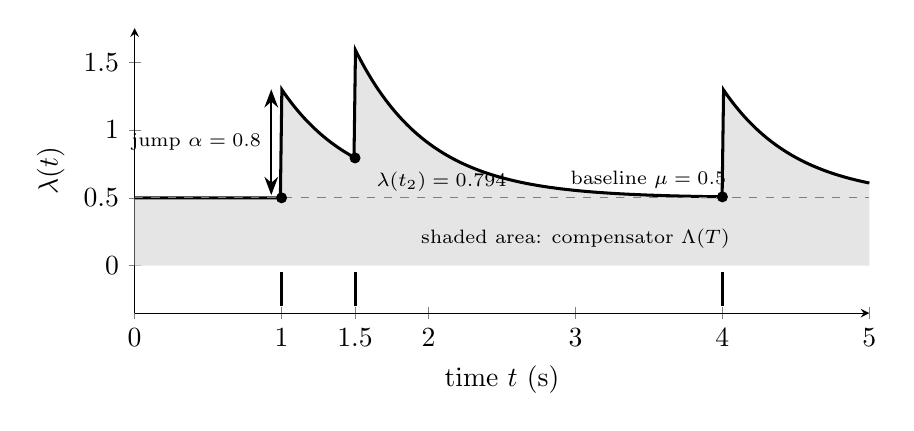
\begin{tikzpicture}
\begin{axis}[width=0.9\linewidth,height=5.2cm,xmin=0,xmax=5,ymin=-0.35,ymax=1.75,
  axis lines=left,xlabel={time $t$ (s)},ylabel={$\lambda(t)$},
  ytick={0,0.5,1,1.5},xtick={0,1,1.5,2,3,4,5},
  every axis plot/.append style={line width=1.1pt},clip=false]
  \addplot[name path=lam,color=black,samples=500,domain=0:5]
    {0.5+(x>1)*0.8*exp(-2*max(x-1,0))+(x>1.5)*0.8*exp(-2*max(x-1.5,0))+(x>4)*0.8*exp(-2*max(x-4,0))};
  \addplot[name path=zero,draw=none,domain=0:5]{0};
  \addplot[gray!20] fill between[of=lam and zero];
  \addplot[gray,dashed,thin,domain=0:5]{0.5};
  \node[font=\scriptsize,anchor=south west] at (axis cs:2.9,0.5) {baseline $\mu=0.5$};
  \foreach \t/\l in {1/0.5,1.5/0.794,4/0.507}{
    \edef\temp{\noexpand\draw[line width=1.1pt] (axis cs:\t,-0.3) -- (axis cs:\t,-0.05);
      \noexpand\fill (axis cs:\t,\l) circle (2pt);}
    \temp}
  \node[font=\scriptsize,anchor=north west] at (axis cs:1.58,0.76) {$\lambda(t_2)=0.794$};
  \draw[{Stealth}-{Stealth},thick] (axis cs:0.93,1.30) -- node[left,font=\scriptsize]{jump $\alpha=0.8$} (axis cs:0.93,0.52);
  \node[font=\scriptsize,align=center] at (axis cs:3.0,0.2) {shaded area: compensator $\Lambda(T)$};
\end{axis}
\end{tikzpicture}
\caption{Intensity of a univariate Hawkes process with \(\mu=0.5\), \(\alpha=0.8\) and
\(\beta=2\), for three events (ticks on the axis). Each event adds a jump that decays with
half-life \(\ln 2/2\approx0.35\)~s. The dots are the intensities at the events, the terms
that the likelihood rewards; the shaded area is the compensator, the term it penalizes.}
\label{fig:intensity}
\end{figure}

\paragraph{The intensity as a state.} Write \(E(t)=\lambda(t)-\mu\) for the excitation.
Between events, \(E\) decays as \(\mathrm dE/\mathrm dt=-\beta E\); at an event it jumps by
\(\alpha\). Hence, with \(\Delta_k=t_k-t_{k-1}\),
\begin{equation}
  E(t_k^-)=e^{-\beta\Delta_k}\bigl(E(t_{k-1}^-)+\alpha\bigr),
  \label{eq:recursion}
\end{equation}
and the current intensity summarizes the whole past: with an exponential kernel the
process \(\lambda(t)\) is Markov. This property makes simulation and the likelihood linear
in the number of events. It does not hold for other kernels, such as the power law, where
the whole history must be kept.

\paragraph{Cluster representation.} The same process can be generated as a population
\citep{hawkes2018,laub2021}. Immigrants arrive as a Poisson process of rate \(\mu\); each
event, immigrant or not, produces children as an inhomogeneous Poisson process of rate
\(\alpha e^{-\beta s}\), where \(s\) is the time since the parent. The number of direct
children of an event is Poisson with mean
\[
  g=\int_0^\infty\alpha e^{-\beta s}\,\mathrm ds=\frac{\alpha}{\beta},
\]
which is why \(g\) is called the branching ratio. Children, grandchildren and further
generations form a geometric series, so the mean size of the cluster started by one
immigrant is
\[
  1+g+g^2+\cdots=\frac{1}{1-g}\qquad(g<1),
\]
and a fraction \(g\) of all events is endogenous, triggered by earlier events rather than by
the baseline. Taking expectations in Equation~\eqref{eq:hawkes1d}, the stationary mean rate
\(\bar\lambda=\E[\lambda(t)]\) satisfies \(\bar\lambda=\mu+g\bar\lambda\), that is,
\(\bar\lambda=\mu/(1-g)\). Only the times are observed; the genealogy
(Figure~\ref{fig:cluster}) is latent.

\begin{figure}[htbp]
\centering
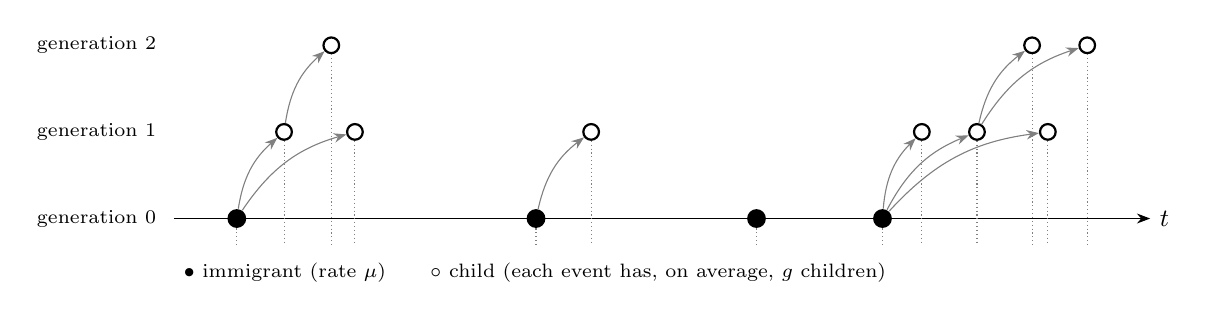
\begin{tikzpicture}[x=1.0cm,y=1.1cm,
  imig/.style={circle,fill=black,inner sep=2.4pt},
  child/.style={circle,draw=black,fill=white,thick,inner sep=2pt},
  link/.style={-{Stealth[length=1.6mm]},gray,thin}]
  \draw[-{Stealth}] (0,0) -- (12.4,0) node[right,font=\small]{$t$};
  \node[imig] (a) at (0.8,0) {};
  \node[child] (a1) at (1.4,1) {}; \node[child] (a2) at (2.3,1) {};
  \node[child] (a11) at (2.0,2) {};
  \draw[link] (a) to[bend left=20] (a1); \draw[link] (a) to[bend left=20] (a2);
  \draw[link] (a1) to[bend left=20] (a11);
  \node[imig] (b) at (4.6,0) {};
  \node[child] (b1) at (5.3,1) {};
  \draw[link] (b) to[bend left=20] (b1);
  \node[imig] (c) at (7.4,0) {};
  \node[imig] (d) at (9.0,0) {};
  \node[child] (d1) at (9.5,1) {}; \node[child] (d2) at (10.2,1) {}; \node[child] (d3) at (11.1,1) {};
  \node[child] (d21) at (10.9,2) {}; \node[child] (d22) at (11.6,2) {};
  \draw[link] (d) to[bend left=20] (d1); \draw[link] (d) to[bend left=20] (d2); \draw[link] (d) to[bend left=20] (d3);
  \draw[link] (d2) to[bend left=20] (d21); \draw[link] (d2) to[bend left=20] (d22);
  \foreach \p in {a,a1,a2,a11,b,b1,c,d,d1,d2,d3,d21,d22}{\draw[densely dotted,gray] (\p) -- (\p|-{(0,-0.3)});}
  \foreach \y in {0,1,2}{\node[font=\scriptsize,anchor=east] at (-0.1,\y) {generation \y};}
  \node[font=\scriptsize,anchor=north west] at (0,-0.4) {$\bullet$ immigrant (rate $\mu$)\qquad
    $\circ$ child (each event has, on average, $g$ children)};
\end{tikzpicture}
\caption{Cluster representation of a Hawkes process. Only the projection of the events on
the time axis is observed; which event triggered which is hidden. With \(g=0.5\), each
immigrant brings on average a cluster of \(1/(1-0.5)=2\) events.}
\label{fig:cluster}
\end{figure}

\section{Symmetric bivariate Hawkes process}

A \(D\)-dimensional Hawkes process has one intensity per type,
\[
 \lambda_i(t)=\mu_i+\sum_{j=1}^{D}\int_{(0,t)}\phi_{ij}(t-s)\,\mathrm dN_j(s),
 \qquad i=1,\dots,D,
\]
where \(\phi_{ij}\) is the effect of a type-\(j\) event on the intensity of type \(i\)
\citep{hawkes1971b,bacry2015}. With exponential kernels and two types there are, in general,
two baselines, four jump sizes and up to four decay rates. Here,
up-moves and down-moves are processes \(N_1,N_2\) with a common decay and symmetric
excitation:
\begin{align}
\lambda_1(t)&=\mu+\sum_{t_k^1<t}\alpha_{\mathrm{self}}e^{-\beta(t-t_k^1)}
 +\sum_{t_k^2<t}\alpha_{\mathrm{cross}}e^{-\beta(t-t_k^2)},\\
\lambda_2(t)&=\mu+\sum_{t_k^2<t}\alpha_{\mathrm{self}}e^{-\beta(t-t_k^2)}
 +\sum_{t_k^1<t}\alpha_{\mathrm{cross}}e^{-\beta(t-t_k^1)}.
\end{align}
The model reduces a general matrix to four parameters. This parsimony makes
simulation and comparison with \citet{lee2023} easier. Figure~\ref{fig:bivariate} draws it
as a diagram of the two event types. An up-move raises the intensity of another up-move by
\(\alpha_{\mathrm{self}}\) and that of a down-move by \(\alpha_{\mathrm{cross}}\), and
symmetrically for a down-move; both increases decay at the same rate \(\beta\). In
microstructure, dominant cross-excitation indicates reversion (an up-move followed by a
down-move), and dominant self-excitation indicates persistence of direction
\citep{bacry2013}.

\begin{figure}[htbp]
\centering
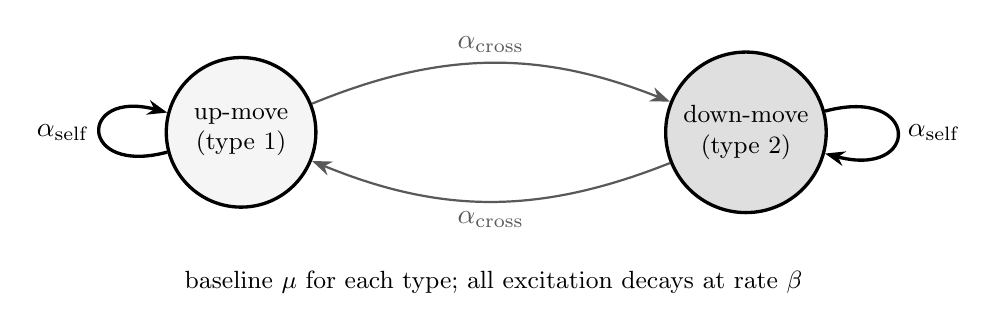
\begin{tikzpicture}[node distance=4.4cm,
  ev/.style={circle,draw=black,very thick,minimum size=1.9cm,font=\small,align=center}]
  \node[ev,fill=gray!8] (u) {up-move\\(type 1)};
  \node[ev,fill=gray!25,right=of u] (d) {down-move\\(type 2)};
  \draw[-{Stealth[length=2.5mm]},very thick] (u) edge[loop left,looseness=6]
    node[left]{$\alpha_{\mathrm{self}}$} (u);
  \draw[-{Stealth[length=2.5mm]},very thick] (d) edge[loop right,looseness=6]
    node[right]{$\alpha_{\mathrm{self}}$} (d);
  \draw[-{Stealth[length=2.5mm]},thick,gray!70!black] (u) to[bend left=22]
    node[above]{$\alpha_{\mathrm{cross}}$} (d);
  \draw[-{Stealth[length=2.5mm]},thick,gray!70!black] (d) to[bend left=22]
    node[below]{$\alpha_{\mathrm{cross}}$} (u);
  \node[font=\small] at ($(u)!0.5!(d)+(0,-1.9)$) {baseline $\mu$ for each type; all excitation decays at rate $\beta$};
\end{tikzpicture}
\caption{The symmetric bivariate Hawkes process as a diagram of event types. Loops are
self-excitation, arrows between types are cross-excitation; the same four parameters
\((\mu,\alpha_{\mathrm{self}},\alpha_{\mathrm{cross}},\beta)\) apply to both types.
\(\alpha_{\mathrm{self}}>\alpha_{\mathrm{cross}}\) describes persistence of direction, as
found in the crypto data of this work; \(\alpha_{\mathrm{cross}}>\alpha_{\mathrm{self}}\)
describes reversion, as at the equity fixed point of \citet{lee2023}.}
\label{fig:bivariate}
\end{figure}

\section{Stability}

The mass matrix of the kernels is
\[
 \mathbf G=\frac{1}{\beta}
 \begin{bmatrix}
  \alpha_{\mathrm{self}} & \alpha_{\mathrm{cross}}\\
  \alpha_{\mathrm{cross}} & \alpha_{\mathrm{self}}
 \end{bmatrix}.
\]
Its entry \((i,j)\) is the mean number of type-\(i\) children of a type-\(j\) event, so
\(\mathbf G\) plays the role of the branching ratio. Its eigenvalues are
\((\alpha_{\mathrm{self}}-\alpha_{\mathrm{cross}})/\beta\) and the largest,
\[
 g=\frac{\alpha_{\mathrm{self}}+\alpha_{\mathrm{cross}}}{\beta},
\]
which is the mean number of children of either type per event. The two eigenvalues have
eigenvectors \((1,1)\) and \((1,-1)\): the first governs the total activity
\(N_1+N_2\), the second the difference \(N_1-N_2\), that is, the price
(Section~\ref{sec:volatility-theory}). Write
\[
 g_-=\frac{\alpha_{\mathrm{self}}-\alpha_{\mathrm{cross}}}{\beta}
\]
for the second eigenvalue. The condition \(g<1\) is
required. Close to one, cascades last longer; above one, there is no usual stationary
regime \citep{hardiman2013,filimonov2012}. Under stationarity, by the same argument as in
the univariate case, each type occurs at mean rate \(\mu/(1-g)\), and the two together at
\(2\mu/(1-g)\).

\section{Marks and price}

An event has a time, a type and a mark. The mark is the size of the change in ticks.
The paper keeps the mark for volatility, but assumes that the intensity does not
depend on it. The filtered price can be written, in ticks, as the cumulative
difference between up-moves and down-moves.

\section{Volatility}
\label{sec:volatility-theory}

In a minimal model, if the price moves by one tick \(\vartheta\) at a rate \(\phi\),
\[
 \sigma^2\approx\phi\vartheta^2.
\]
Thus, modeling intensity is modeling activity and, consequently, a component of
volatility. The marked Hawkes expression requires moments of the marks and the
estimated parameters \citep{leeseo2017,lee2024}.

\paragraph{Long-run variance of the Hawkes price.} With unit marks the price is
\(X(t)=N_1(t)-N_2(t)\), the projection on the eigenvector \((1,-1)\). Under stationarity each
type has mean rate \(\bar\lambda=\mu/(1-g)\), and the variance of \(X\) per unit time
converges, as the horizon grows, to
\[
 \lim_{T\to\infty}\frac{\Var X(T)}{T}=\frac{2\bar\lambda}{(1-g_-)^2}
\]
\citep{bacry2013}. If each event moves the price by an i.i.d.\ size \(J\), independent of the
times, with the sign given by the type, the same argument gives
\begin{equation}
 \sigma_H^2=2\bar\lambda\left[\Var(J)+\frac{\E[J]^2}{(1-g_-)^2}\right],
 \label{eq:hawkes-variance}
\end{equation}
the expression used in Section~\ref{sec:real-volatility}. The total activity depends on
\(g\), and the amplification of the variance on \(g_-\). When self-excitation dominates,
\(g_->0\) and moves in the same direction cluster, so the variance exceeds that of a Poisson
price with the same activity. When cross-excitation dominates, \(g_-<0\), moves tend to undo
each other and the variance falls below it; this is the mechanism that \citet{bacry2013} use
to model microstructure noise. When \(\alpha_{\mathrm{self}}=\alpha_{\mathrm{cross}}\), the
long-run variance equals that of the difference of two independent Poisson processes with the
same activity.

\paragraph{Realized volatility.} The benchmark is the realized variance over a window,
\[
 \mathrm{RV}_\Delta=\sum_k r_k^2,
\]
the sum of squared log returns sampled every \(\Delta\) seconds
\citep{andersen2003,barndorff2002}. Without noise, it converges to the integrated variance as
\(\Delta\to0\). At high frequency, however, the observed price contains microstructure noise,
and \(\mathrm{RV}_\Delta\) is biased upward when \(\Delta\) is small \citep{zhang2005}. The
signature plot, \(\mathrm{RV}_\Delta\) per unit time against \(\Delta\), shows the effect:
noise makes it fall with \(\Delta\), while positively autocorrelated returns, as in a
self-exciting price, make it rise toward the long-run level of
Equation~\eqref{eq:hawkes-variance}.

\section{Simulation}

A Hawkes path can be simulated by Ogata's thinning \citep{ogata1981}. If
\(\lambda(t)\le M\) on an interval, candidates are drawn from a Poisson process of rate
\(M\) and each candidate at time \(s\) is kept with probability \(\lambda(s)/M\); the kept
points have intensity \(\lambda\). With an exponential kernel the intensity only decreases
between events, so its value just after the last event is a valid bound until the next
event. In the bivariate case the bound is \(\lambda_1+\lambda_2\), and the type of an
accepted event is drawn in proportion to \(\lambda_1\) and \(\lambda_2\). The
implementation is described in Section~\ref{sec:sim-thinning}.

\section{Maximum likelihood}
\label{sec:mle-theory}

For a horizon \(T\),
\[
 \ell(\theta)=\sum_k\log\lambda_{c_k}(t_k)
 -\sum_i\int_0^T\lambda_i(u)\,du.
\]
The first term rewards high intensity at the events; the second penalizes high
intensity over the whole interval. Maximizing only the first would drive the
intensities to infinity. The compensator provides the balance. For an exponential
kernel, the sum over the past obeys a first-order recursion, and \(\ell\) and its
gradient can be computed in \(O(n)\) operations \citep{ozaki1979}. In the univariate case,
let \(A_1=0\) and \(A_k=e^{-\beta(t_k-t_{k-1})}(1+A_{k-1})\), so that \(\alpha A_k\) is
the excitation just before \(t_k\) (Equation~\eqref{eq:recursion}). Then
\begin{equation}
 \ell(\mu,\alpha,\beta)=\sum_{k=1}^{n}\log\bigl(\mu+\alpha A_k\bigr)-\mu T
 -\frac{\alpha}{\beta}\sum_{k=1}^{n}\Bigl(1-e^{-\beta(T-t_k)}\Bigr).
 \label{eq:loglik1d}
\end{equation}
The bivariate likelihood has the same structure, with one recursion per pair of source and
target types. Under regularity conditions, the MLE is consistent and asymptotically
efficient \citep{ogata1978}: approximately normal around the true value, with covariance
given by the inverse Fisher information, which the inverse of the observed Hessian of
\(-\ell\) estimates. These conditions include a true parameter in the interior of the
parameter space. When it lies on the boundary, as \(\alpha_{\mathrm{cross}}=0\), the
estimate piles up at the boundary with positive probability, and neither the normal
approximation nor the usual \(\chi^2\) reference for likelihood ratio tests applies
\citep{selfliang1987}. This is relevant for the real data of this work, where
\(\alpha_{\mathrm{cross}}\) is estimated close to zero.

\section{Model comparison}

The Poisson process is nested in the Hawkes process: it is the case
\(\alpha_{\mathrm{self}}=\alpha_{\mathrm{cross}}=0\). The likelihood ratio statistic
\(2(\hat\ell_{\mathrm{Hawkes}}-\hat\ell_{\mathrm{Poisson}})\) measures the gain in fit. Its
usual \(\chi^2\) reference does not hold here for two reasons: the null value lies on the
boundary of the parameter space \citep{selfliang1987}, and \(\beta\) has no effect under the
null, so it is not identified there. The Akaike information criterion,
\[
 \mathrm{AIC}=2k-2\hat\ell,
\]
with \(k\) the number of free parameters, compares the two fits with a penalty for the extra
parameters \citep{akaike1974}. A difference in AIC of hundreds of units, as found on the real
windows, leaves no doubt about the direction, whatever the exact reference distribution.

\section{Goodness of fit by time rescaling}
\label{sec:time-rescaling}

If the model is correct, the compensator turns the observed process into a unit-rate
Poisson process: the transformed times \(\Lambda(t_k)\) are the events of a homogeneous
Poisson process of rate one. This is the time-rescaling theorem \citep{brown2002}. The
increments
\[
 \tau_k=\Lambda(t_k)-\Lambda(t_{k-1})=\int_{t_{k-1}}^{t_k}\lambda(u)\,\mathrm du
\]
are then independent \(\mathrm{Exp}(1)\) variables. In the bivariate case the theorem
applies to each type with its own compensator \(\Lambda_i\). Evaluated at the estimated
parameters, the \(\tau_k\) are the rescaled residuals of the fit \citep{ogata1988}. Their
distribution is tested against \(\mathrm{Exp}(1)\), for example with Kolmogorov--Smirnov,
and their serial dependence with Ljung--Box. A kernel of the wrong shape typically leaves
dependence in the residuals: bursts that the fitted kernel forgets too fast or too slowly
appear as runs of short or long \(\tau_k\).

\section{Observation on a time grid}

The events of this work are changes of the mid-price recorded on a 100~ms grid
(Chapter~\ref{cap:dados}). Two things are lost relative to continuous time: event times are
rounded to the grid, and changes that fall in the same cell merge into one. The second
matters most for the decay. With \(\beta\) of a few units per second, much of the excitation
acts within a few hundred milliseconds, and merged events remove part of the short
inter-arrivals from which \(\beta\) is identified. A likelihood written for continuous time
therefore estimates the parameters of the process as seen through the grid, with \(\beta\)
biased downward; Section~\ref{sec:addendum-grid} measures the size of this bias.
Likelihoods that account for the observation scheme have been proposed for this setting
\citep{lambe2025}.

A biased estimator can still be corrected by simulation, the idea of indirect inference
\citep{gourieroux1993}. Let \(b(\theta)\) be a summary, such as the median, of the grid MLE
over paths simulated from \(\theta\) in continuous time and mapped to the grid. The map
\(b\) is estimated by simulation, and an estimate on the grid is corrected by solving
\(b(\theta)=\hat\theta_{\mathrm{grid}}\). The correction is as good as the model used to
simulate: if the real process is not a Hawkes process, the map transfers its bias with it.
A network trained on gridded paths with the continuous-time parameter as target learns a
correction of the same kind, conditional on the whole path.

\section{Identifiability in finite samples}
\label{sec:identificabilidade}

The asymptotic properties do not guarantee good behavior with 1,000 events. When the
excitation is weak (small \(\alpha_{\mathrm{self}}+\alpha_{\mathrm{cross}}\)), the
kernel barely changes the intensity, and the likelihood becomes flat in the direction
of \(\beta\): very different values of \(\beta\) explain the data almost equally well.
In the limit \(\alpha\to0\), \(\beta\) is no longer identified. Near criticality, the
separation between \(\mu\) and \(g\) also deteriorates, because the mean rate
\(2\mu/(1-g)\) is well determined, but neither factor is on its own. These effects
reappear in the results of Chapter~\ref{cap:resultados}.

\section{Amortized estimation as a Bayes estimator}
\label{sec:bayes}

In the approach of \citet{lee2023}, a network \(f_\phi\) is trained on pairs
\((\theta_i,x_i)\), where \(\theta_i\) is drawn from a training distribution \(\pi\)
and \(x_i\) is simulated from the model with parameter \(\theta_i\). Minimizing the
mean squared error,
\[
  \min_\phi\;\E_{\theta\sim\pi}\,\E_{x\mid\theta}
  \bigl\lVert f_\phi(x)-\theta\bigr\rVert^2,
\]
is minimizing the Bayes risk under squared loss, whose solution is the posterior mean
\(\E_\pi[\theta\mid x]\) \citep{lehmann1998}. Hence, a well-trained network
approximates a Bayes estimator under the prior \(\pi\)
\citep{sainsburydale2024,lenzi2023}. Two consequences guide this work. First, on a
test set drawn from the same \(\pi\), no estimator has lower average MSE than the
posterior mean, so outperforming the MLE on that test is expected and does not prove
superiority in a frequentist sense. Second, the network does not extrapolate: its
estimates shrink toward the high-density region of \(\pi\), and real data outside the
support of the prior yield biased estimates.

The same approach belongs to a wider family of amortized, simulation-based inference methods,
in which the cost of inference is paid once, in training, and each new data set costs a
forward pass \citep{cranmer2020,radev2022}. On real windows the target changes. When a
network is trained on pairs \((x,\hat\theta_{\mathrm{MLE}}(x))\), the label is a deterministic
function of the input, so the minimizer of the squared loss is the MLE itself: the network
becomes a fast approximation of the MLE map, accurate where the training windows are dense.
Starting from the weights trained on simulated data, it can reach that approximation with
fewer real windows; how close the simulation prior is to the real data then matters for how
much that initialization helps.

\section{Comparing estimators}
\label{sec:comparing-theory}

The estimators are compared path by path. For each path or window \(i\), a loss
\(L_i(A)\), such as the squared error averaged over the four parameters, is computed for each
estimator \(A\); the macro MSE is the average of the per-parameter MSEs. Two estimators are
compared through the paired differences \(d_i=L_i(A)-L_i(B)\). Pairing removes the variation
in difficulty between paths, which is often much larger than the difference between
estimators.
The mean \(\bar d\) is reported with a bootstrap confidence interval, obtained by resampling
the \(d_i\) with replacement \citep{efron1993}, and the null hypothesis of no difference is
tested with the Wilcoxon signed-rank test, which uses the ranks of \(|d_i|\) and is robust to
the heavy tails of squared errors \citep{wilcoxon1945,diebold1995}. Variation across training
seeds is a different source: it measures the instability of training, not the accuracy of a
trained model, and is compared across seeds \citep{bouthillier2021}.

When several comparisons are tested together, the Holm procedure controls the probability
of any false rejection: with the \(m\) \(p\)-values sorted in increasing order, the \(k\)-th
is compared with \(0.05/(m-k+1)\), and testing stops at the first non-rejection
\citep{holm1979}. Agreement between two orderings, such as the Hawkes and the realized
volatilities across windows, is measured by the Spearman correlation, the correlation of the
ranks, which ignores the level and depends only on the order.

\paragraph{Ensembles.} The average \(\bar y=\frac1M\sum_m y_m\) of \(M\) estimators satisfies
\[
 \lVert\bar y-\theta\rVert^2=\frac1M\sum_{m=1}^{M}\lVert y_m-\theta\rVert^2
 -\frac1M\sum_{m=1}^{M}\lVert y_m-\bar y\rVert^2
\]
\citep{krogh1995}. The error of the average equals the average error of the members minus
their spread, so it is never worse than the average member, and it improves most when the
members are accurate and err in different places. This identity applies both to the
ensembles of five seeds and to the average of the LSTM and the Transformer.

\section{LSTM}

Recurrent networks update a state \(h_t=f(x_t,h_{t-1})\). The LSTM introduces input,
forget and output gates to control the flow of information and mitigate the
vanishing gradient problem \citep{hochreiter1997}. With \(\sigma\) the logistic function
and \(\odot\) the elementwise product,
\begin{align*}
 f_t&=\sigma(W_f[h_{t-1},x_t]+b_f), & i_t&=\sigma(W_i[h_{t-1},x_t]+b_i),\\
 o_t&=\sigma(W_o[h_{t-1},x_t]+b_o), & \tilde c_t&=\tanh(W_c[h_{t-1},x_t]+b_c),\\
 c_t&=f_t\odot c_{t-1}+i_t\odot\tilde c_t, & h_t&=o_t\odot\tanh(c_t).
\end{align*}
The cell state \(c_t\) is updated additively, which lets gradients pass over many steps.
The update has the form of Equation~\eqref{eq:recursion}: a forget gate that depends on the
inter-arrival time can play the role of \(e^{-\beta\Delta_k}\), and the input gate that of
the jump, so an LSTM can represent the excitation of a Hawkes process in its state. In
Lee, the sequence contains the inter-arrival time and the type; the final state feeds the
regression of the four parameters. The paper also tested a GRU \citep{cho2014}, with
slightly worse results.

\section{Attention and the Transformer}

Attention computes weighted combinations:
\[
 \operatorname{Attention}(Q,K,V)=
 \operatorname{softmax}\left(\frac{QK^\top}{\sqrt{d_k}}\right)V.
\]
Each position queries all the others. The Transformer combines multiple heads,
feed-forward layers, residual connections and normalization \citep{vaswani2017}. Each head
applies its own projections \(Q=XW^Q\), \(K=XW^K\), \(V=XW^V\) to the sequence \(X\), and
the heads are concatenated. Self-attention is equivariant to permutations of the sequence,
so order and spacing must enter through a positional encoding; for a point process the
relevant position is the time of each event, not only its index. The
potential advantage is capturing distant dependencies; the potential cost is
\(O(n^2)\) memory. The position of the normalization relative to the residual
connections affects training stability: the \emph{post-LN} variant, used here,
usually requires learning-rate warm-up \citep{xiong2020}.

\section{Training}

The networks are trained by stochastic gradient descent on mini-batches with Adam, which
scales each step by running estimates of the first and second moments of the gradient
\citep{kingma2015}. The learning rate can follow a schedule, such as a short warm-up or a cosine decay
\citep{xiong2020,loshchilov2017}. Training stops at a fixed budget of epochs or when the
validation loss stops improving, and the checkpoint with the lowest validation loss is kept;
the test data are not used for any choice. Fine-tuning reuses this procedure from weights
already trained on another task, here the simulated paths, with the real windows as the new
training set.

\chapter{Related Work}

\section{Hawkes processes in finance}

After the original formulation \citep{hawkes1971,hawkes1971b}, self- and mutually
exciting models came to describe market events in continuous time
\citep{bowsher2007,embrechts2011}, contagion between markets \citep{aitsahalia2015}
and endogeneity, measured by the branching ratio \citep{filimonov2012,hardiman2013}.
\citet{bacry2013} use a bivariate Hawkes process of up- and down-moves to reproduce
the microstructure noise of the price; cross-excitation captures reversion at short
scales. \citet{bacry2015} and \citet{hawkes2018} review this field, and
\citet{mutoke2011} offers a didactic introduction. \citet{leeseo2017} connect the
marked Hawkes process to the price in ticks and derive Hawkes volatility, which
\citet{lee2024} apply to filtered prices. In Brazil, \citet{primo2018} analyzes the
intraday clustering of stocks with MLE, and \citet{silva2026} systematizes inference,
diagnostics and financial applications.

\section{Estimation of Hawkes processes}

MLE for exponential kernels dates back to \citet{ozaki1979}, with asymptotic
properties established by \citet{ogata1978}. Simulation by \emph{thinning}
\citep{ogata1981} and diagnostics by rescaled residuals \citep{ogata1988,brown2002}
complete the classical toolbox \citep{laub2021}. The optimization is sensitive to the
initialization and to the geometry of the likelihood, which can be nearly flat in
some directions when the series is short (Section~\ref{sec:identificabilidade}).

\section{Amortized and simulation-based inference}

When the likelihood is expensive or intractable, networks trained on simulations
replace the optimization with a single forward pass \citep{cranmer2020}. Networks
trained on simulations already estimate parameters of spatial and extreme-value
models \citep{gerber2021,lenzi2023}; with squared loss, they approximate Bayes
estimators \citep{sainsburydale2024}, and methods such as BayesFlow learn the full
posterior \citep{radev2022}. \citet{lee2023} applies the idea to the 2D Hawkes process
with an LSTM. \citet{lambe2025} use networks for the Hawkes process observed only
through interval counts, a case in which the exact likelihood is intractable and the
MLE is no longer a direct alternative.

\section{Neural point processes}

Another line of work uses networks to model the intensity itself, without the
parametric form of Hawkes: RMTPP \citep{du2016}, the Neural Hawkes Process
\citep{mei2017} and attention-based variants such as the Transformer Hawkes Process
\citep{zuo2020} and the Self-Attentive Hawkes Process \citep{zhang2020};
\citet{shchur2021} review the area. The goal differs from that of this work: those
models maximize predictive likelihood, whereas here the network estimates the four
interpretable parameters of a classical model.

\section{Hawkes processes in crypto-assets}

Using one-minute returns of 17 cryptocurrencies traded on Binance,
\citet{taddeo2024} show that Hawkes describes the occurrence of jumps in log-returns
better than Poisson. The crypto market also exhibits segmentation and limited
arbitrage across exchanges \citep{makarov2020}, and perpetual futures, which have no
expiry and carry a funding rate, concentrate a large share of the liquidity
\citep{he2022perpetual}.

\section{Positioning}

\begin{table}[htbp]
\centering
\caption{Positioning of this work relative to the closely related literature.}
\label{tab:posicionamento}
\small
\begin{tabularx}{\linewidth}{lllX}
\toprule
Work & Estimation & Architecture & Market\\
\midrule
\citet{bacry2013} & MLE & -- & futures (Bund, DAX)\\
\citet{leeseo2017} & MLE & -- & equities\\
\citet{primo2018} & MLE & -- & equities (Brazil)\\
\citet{taddeo2024} & MLE & -- & crypto (jumps in 1-min returns)\\
\citet{lee2023} & network & LSTM & equities (US)\\
\citet{lambe2025} & network & MLP & synthetic (counts)\\
\citet{zuo2020} & neural intensity & Transformer & generic\\
This work & network and MLE & LSTM and Transformer & crypto (perpetual futures)\\
\bottomrule
\end{tabularx}
\end{table}

The present work combines controlled reproduction, public crypto data and a
comparison with attention, and adds to the evaluation of \citet{lee2023} robust
metrics, paired tests and the interpretation of the network as a Bayes estimator.

\chapter{Data}
\label{cap:dados}

\section{Source and market}

Both spot and futures were evaluated. The need for the best bid/ask ruled out the
official spot archive, which has no equivalent historical \dataset{bookTicker}. USD-M
futures provide \dataset{bookTicker} and \dataset{aggTrades}. The symbols are BTCUSDT
and ETHUSDT \citep{binancePublicData}.

\section{Schema}

\dataset{bookTicker} includes an identifier, the best bid and ask prices and
quantities, the transaction time and the event time. The canonical schema has a UTC
timestamp, bid, ask and quantities. Audits check for positive prices, bid less than
or equal to ask, ordering and temporal duplicates.

\section{Sampling}

Updates can occur every millisecond, a much finer resolution than the chosen scale.
Timestamps are grouped into 100 ms bins and the last state is kept. This filter
follows Lee's protocol and reduces ultra-high-frequency noise.

\section{Datasets produced}

\begin{table}[htbp]
\centering
\caption{Dataset coverage.}
\label{tab:cobertura}
\begin{tabular}{lrrr}
\toprule
Window & Symbol-days & Events & Segments of 1,000\\
\midrule
Primary (Jan.\ 2024) & 28 & 1,826,904 & 1,813\\
Robustness (Oct.\ 2023) & 14 & 1,288,352 & 1,281\\
\bottomrule
\end{tabular}
\end{table}

\section{Event characteristics}
\label{sec:caracteristicas}

Table~\ref{tab:caracteristicas} summarizes the events of the calibration block
(January 15 to 22, 2024). Three facts distinguish these data from the setting of
\citet{lee2023}. First, about 76\% of the changes repeat the direction of the previous
one, which indicates persistence rather than reversion. Second, the median jump is 10
to 15 ticks and only 10--13\% of the jumps are one tick: at the 100~ms scale, these
contracts behave as small-tick assets. Third, 37--39\% of the inter-arrival times are
exactly 0.1~s, the grid step; the sampling strongly discretizes the times, whereas the
model and the simulations assume continuous time.

\begin{table}[htbp]
\centering
\caption{Characteristics of the mid-price events, January 15 to 22, 2024.}
\label{tab:caracteristicas}
\small
\begin{tabular}{lrr}
\toprule
 & BTCUSDT & ETHUSDT\\
\midrule
Events & 529,278 & 540,164\\
Fraction of up-moves & 49.4\% & 49.5\%\\
Probability of repeating the previous direction & 76.0\% & 75.7\%\\
Median inter-arrival time & 0.3 s & 0.3 s\\
Inter-arrival times equal to 0.1 s (grid) & 39.5\% & 37.3\%\\
Median / 90th percentile jump (ticks) & 15.5 / 48 & 10 / 29\\
One-tick jumps & 9.7\% & 12.6\%\\
\bottomrule
\end{tabular}
\end{table}

\chapter{Methodology}

\section{Principles}

The protocol distinguishes:
\begin{description}
  \item[R1:] explicitly published information;
  \item[R2:] reconstruction to fill a gap;
  \item[A1:] adaptation required for crypto;
  \item[E1:] extension with a Transformer.
\end{description}

\section{Pipeline}

\begin{enumerate}
  \item build the daily URL and download the ZIP;
  \item compute the SHA-256 and record it in a manifest;
  \item temporarily extract the CSV;
  \item process chunks of one million rows;
  \item reduce the updates to the 100 ms grid;
  \item produce Parquet partitioned by symbol and date;
  \item delete the temporary CSV;
  \item create windows without crossing splits;
  \item fit the MLE and calibrate ranges on the training set only;
  \item generate synthetic paths and train the estimators;
  \item select hyperparameters on the validation set;
  \item open the test set only once.
\end{enumerate}

\section{Simulation by thinning}
\label{sec:sim-thinning}

Given the current state, an upper bound on the sum of the intensities is computed. An
exponential waiting time is drawn; the excitation decays; the candidate is accepted
with probability proportional to the new intensity \citep{ogata1981}. The type is
drawn with probabilities proportional to \(\lambda_1,\lambda_2\). After the event, the
corresponding column of the \(\alpha\) matrix is added. Each path starts with an
empty history, the same assumption as in the likelihood.

\section{Constrained MLE}

Positive parameters are obtained through softplus. Instead of optimizing \(\beta\)
freely, a positive margin \(d\) is used:
\[
(\mu,\alpha_s,\alpha_c,d)=\softplus(z),\qquad
\beta=\alpha_s+\alpha_c+d.
\]
L-BFGS-B is started from five points: one based on the empirical event rate and four
random perturbations in the unconstrained space. The MLE never receives the true
parameter as initialization. The gradient is analytic, and the exponential
recursions are solved as bidiagonal systems. Convergence, iterations, log-likelihood
and time are recorded.

\section{Neural protocol}

The target is \((\mu,\alpha_s,\alpha_c,\beta)\), and the loss is the MSE on the
original scale. The input for each event is \((\log(1+\Delta t),\,s)\), with \(s=+1\)
for an up-move and \(s=-1\) for a down-move; Lee uses inter-arrival times and types
1/2, so this transformation is a reconstruction (R2). The two networks share the
output head: softplus produces \(\mu,\alpha_s,\alpha_c,d>0\) and
\(\beta=\alpha_s+\alpha_c+d\), which guarantees \(g<1\) by construction, as in Lee's
robust version.

The frozen synthetic experiment contains 75,000 training sequences, 10,000 validation
sequences and 15,000 test sequences, all of exactly 1,000 events. The parameters are
drawn with \(\mu\in[0.2,\,0.6]\), \(\beta\in[0.8,\,2.0]\), self-excited fraction
\(\alpha_s/(\alpha_s+\alpha_c)\in[0.2,\,0.8]\) and \(g\) balanced across three
strata: low \([0.10,\,0.35)\), intermediate \([0.35,\,0.70)\) and near-critical
\([0.70,\,0.95]\). Table~\ref{tab:treino} summarizes the training.

\begin{table}[htbp]
\centering
\caption{Training configuration and cost (five seeds per network, Apple Silicon Mac
with MPS).}
\label{tab:treino}
\small
\begin{tabular}{lrr}
\toprule
 & LSTM (R1/R2) & Transformer (E1)\\
\midrule
Architecture & 2 LSTM $\times$ 12 + dense & encoder, 2 layers, $d=32$\\
Heads / feed-forward & -- & 4 / 128\\
Trainable parameters & 2,068 & 25,700\\
Optimizer & Adam, $10^{-3}$ & Adam, $10^{-3}$\\
Effective batch & 64 & 8 (physical 4 with accumulation)\\
Maximum epochs / patience & 300 / 30 & 300 / 30\\
Best epoch (per seed) & 165, 164, 193, 239, 299 & 73, 42, 38, 60, 44\\
Training time per seed & 5.4--14.8 h & 16.6--28.8 h\\
Total time (5 seeds) & 41 h & 110 h\\
\bottomrule
\end{tabular}
\end{table}

The Transformer's tensor flow starts from \([B,L,2]\), with \(L=1000\). A linear
projection produces \([B,L,32]\), to which the positional encoding is added. In each
layer, the four heads operate in subspaces of dimension eight; the feed-forward block
expands 32 to 128 and returns to 32. Temporal averaging converts \([B,L,32]\) into
\([B,32]\). The memory cost of attention grows quadratically with \(L\), which is why
its batch is smaller than the LSTM's. This difference in batch size, together with the
absence of a hyperparameter search for either network, is a limitation of the
comparison.

\section{The paper's fixed point (E2)}

To compare directly with the sampling-distribution table of \citet{lee2023}, 2,000
paths of 1,000 events were simulated at the published point
\((\mu,\alpha_s,\alpha_c,\beta)=(0.3,\,0.4,\,0.7,\,1.5)\), which lies inside the
training prior. The networks were applied without retraining, and the MLE was fitted
in two versions: the protocol's heuristic and the initialization at the true value
used in the paper.

\section{Empirical protocol}
\label{sec:empirical-protocol}

On real data there is no true parameter, so the empirical stage asks three narrower
questions: whether the Hawkes model describes the windows well enough to be estimated, whether
a network can reproduce the MLE on real windows, and whether the estimated parameters give a
volatility consistent with the realized one. The protocol was fixed in a decision record
(ADR~008) before the test block was opened. The windows have 1,000 events and are split
chronologically by day: calibration (15--22 January 2024, 1,063 windows), validation (23--25
January, 476 windows) and test (26--28 January, 274 windows); the October 2023 week is a
robustness window that is never used for training or selection.

\paragraph{Goodness of fit.} With the MLE of each calibration window, the time-rescaled
residuals of each dimension are tested against \(\mathrm{Exp}(1)\) with Kolmogorov--Smirnov and
for serial dependence with Ljung--Box at 10 lags \citep{ogata1988,brown2002}, and the Hawkes
model is compared with a homogeneous bivariate Poisson process by likelihood ratio and AIC.
Since the times lie on a 100~ms grid, two controls separate the effect of the grid from
misspecification: times jittered uniformly inside their cell with the MLE refitted, and paths
simulated from each fitted model, either in continuous time or mapped to the grid in the same
way as the data. The rejection rate of the simulated controls is what a correct model would
produce.

\paragraph{Networks on real windows.} Each window is labeled with its MLE (five heuristic
starts). Both architectures are trained on the calibration labels with the loss, batch size,
maximum of 300 epochs and patience of 30 of the synthetic protocol, in two variants: from
scratch (Adam, \(10^{-3}\)) and fine-tuned from the synthetic weights of the same seed (Adam,
\(10^{-4}\)), each with the five protocol seeds. Two references need no training: the synthetic
networks as they are, and the mean of the training labels, which is the best constant
predictor. The selected variant is the one whose five-seed ensemble has the lowest macro MSE
on validation. The test block is labeled and read once, after the selection; the stored
weights are evaluated without retraining, and every variant is reported. The machine budget
for this stage was capped at 30 hours.

\paragraph{Volatility.} The long-run volatility implied by the estimated parameters
(Section~\ref{sec:real-volatility}) is compared window by window with the realized volatility
of the log mid-price sampled every \(\Delta\in\{0.1, 1, 5, 10, 30\}\) seconds, using the median
ratio and the Spearman correlation across windows, with \(\Delta=10\)~s as the main horizon,
for the MLE and for the selected network.

\section{Metrics and tests}

The reported metrics are per-parameter and aggregate MSE, median absolute error,
bias, validity, branching-ratio error, cost and MLE convergence. Because the
parameters have different scales, the \(R^2\) of each parameter relative to the prior
mean (the trivial estimator) is also reported. The comparison between networks uses
two sources of variation: across seeds (Welch and Mann--Whitney tests with five
seeds), which measures training variability \citep{bouthillier2021}, and across test
paths (paired difference with a \emph{bootstrap} CI and Wilcoxon test), which measures
the accuracy of the already trained models \citep{efron1993,diebold1995}.

\chapter{Results}
\label{cap:resultados}

\section{Data gate}

All 56 primary files were present. Twenty-eight partitions were generated. BTCUSDT
produced 887,803 events; ETHUSDT, 939,101. The independent window produced 1,288,352
events. The availability and volume gate was therefore satisfied.

\section{Reproduction at the fixed point}

\input{en/e2_fixed_point.tex}

Table~\ref{tab:e2-ponto-fixo} reproduces the qualitative pattern of \citet{lee2023}.
The MLE is practically unbiased, and its standard deviations are about \(\sqrt{2}\)
times those in the paper, as expected for paths of half the length. The networks show
the characteristic shrinkage bias: they pull \(\alpha_{\mathrm{self}}\) and
\(\alpha_{\mathrm{cross}}\) toward the center of the prior, as in the paper, in
exchange for lower variance. The two versions of the MLE produced exactly the same
estimates, so the initialization at the true value used by Lee does not explain the
MLE's advantage at this well-identified point (\(g\approx0.73\)). The macro MSE was
0.0103 for the MLE and 0.0111 for the LSTM ensemble.

\section{Final comparison: LSTM, Transformer and MLE}

\input{en/final_results.tex}

\input{en/posthoc_results.tex}

\section{Computational cost}
\label{sec:custo}

The final run recorded 105~ms of wall-clock time per path for the MLE with four
processes. This value was measured while neural training was occupying the GPU. A
controlled benchmark on the same machine, with the same code (which exactly
reproduces the 15,000 recorded estimates), produced the values in
Table~\ref{tab:custo}.

\begin{table}[htbp]
\centering
\caption{Cost per path of 1,000 events in a controlled benchmark.}
\label{tab:custo}
\small
\begin{tabular}{lr}
\toprule
Estimator and execution mode & Time per path\\
\midrule
MLE, 5 starts, one core & 9.6 ms\\
MLE, 1 start, one core & 2.2 ms\\
MLE, 5 starts, 4 processes (wall-clock) & 2.5 ms\\
LSTM, batch size one, CPU (1 thread) / MPS & 7.0 ms / 29.6 ms\\
Transformer, batch size one, CPU (1 thread / 10 threads) / MPS & 9.9 / 4.8 / 5.0 ms\\
LSTM, batch of 256 on MPS & 0.07 ms\\
Transformer, batch of 32 on MPS & 3.7 ms\\
\midrule
\citet{lee2023}: network / MLE & 12 ms / 1,763 ms\\
\bottomrule
\end{tabular}
\end{table}

With an analytic gradient and a linear recursion, the MLE of this four-parameter
model costs a few milliseconds, the same order as neural inference at batch size one.
The ratio of about 150 times reported by Lee is not reproduced. The cost advantage of
the networks appears in batched inference, especially for the LSTM, and would grow
for models with more expensive likelihoods.

Lee does not describe the implementation of the MLE. To find where its 1,763~ms come from,
the same paths at Lee's fixed point were fitted with implementations that differ in one factor
at a time, at 1,000 and 2,000 events, the two lengths the paper mentions
(Appendix~\ref{ap:lee}). All variants reach the same estimates (largest difference 0.002 in any
parameter); only the cost changes (Table~\ref{tab:custo-variantes}). The likelihood is the
dominant factor: computed as a double sum over pairs of events, it costs about 90 times as much
as the recursion at 2,000 events, while a numerical gradient and a derivative-free optimizer
(Nelder--Mead) multiply the cost by about five each. With the recursion, even an interpreted
loop stays below 0.1~s, and the time reported by Lee falls between the two vectorized
double-sum variants at 2,000 events. The reported ratio is therefore most likely due to a
likelihood computed without the recursion of Section~\ref{sec:mle-theory}.

\begin{table}[htbp]
\centering
\caption{Cost of one MLE fit by implementation, at the fixed point of \citet{lee2023}: median of
10 paths, one start at the true parameters, one core. The pure-Python double sum was timed for
one evaluation and multiplied by the number of evaluations of the vectorized Nelder--Mead fit.}
\label{tab:custo-variantes}
\small
\begin{tabular}{llrr}
\toprule
Likelihood & Gradient and optimizer & 1,000 events & 2,000 events\\
\midrule
Recursion, vectorized & analytic, L-BFGS-B (this work) & 1.1 ms & 1.7 ms\\
Recursion, vectorized & numerical, L-BFGS-B & 5.4 ms & 8.3 ms\\
Recursion, Python loop & numerical, L-BFGS-B & 47 ms & 89 ms\\
Double sum, vectorized & numerical, L-BFGS-B & 176 ms & 711 ms\\
Double sum, vectorized & Nelder--Mead & 818 ms & 3,358 ms\\
Double sum, Python loop & Nelder--Mead (extrapolated) & 26 s & 105 s\\
\midrule
\multicolumn{3}{l}{\citet{lee2023}, implementation not described} & 1,763 ms\\
\bottomrule
\end{tabular}
\end{table}

\section{Empirical calibration}

The MLE converged on all 1,063 calibration windows. The details are in
Section~\ref{sec:calibracao}: cross-excitation is practically zero, \(\beta\) exceeds
the upper limit of the prior in most windows, and no window falls inside all the
ranges used in training. The following sections report the empirical protocol of
Section~\ref{sec:empirical-protocol}.

\input{empirical_results.tex}

\input{addendum_results.tex}

\chapter{Discussion}

\section{Assessment of the hypotheses}

\textbf{H1 --- supported as to structure and volume.} The public data make it
possible to reconstruct sequences with the same structure as Lee's, in sufficient
volume. Their statistical content, however, differs from that of equities: persistent
direction, multi-tick jumps and times discretized by the grid
(Section~\ref{sec:caracteristicas}).

\textbf{H2 --- partially supported.} The LSTM's error is of the same order as the
MLE's: at the fixed point, 0.0111 versus 0.0103; on the synthetic test, the median
per-path loss is practically equal. The substantially lower latency was not confirmed
at batch size one against an efficient MLE (Section~\ref{sec:custo}); it holds for
batched inference.

\textbf{H3 --- not supported on synthetic data.} The Transformer did not reduce the
error: its mean macro MSE was higher than the LSTM's, with no significance across
seeds, and the Transformer ensemble lost to the LSTM ensemble in every regime. Nor
did it perform better in the near-critical regime, where long memory would be most
relevant. Its advantage was latency on MPS (5 ms versus 30 ms for the LSTM), at the
cost of 2.7 times longer training. The result holds for the configuration tested;
there was no hyperparameter search, and the \emph{post-LN} Transformer was trained
without learning-rate warm-up. On real windows, the fine-tuned architectures are indistinguishable on the test block, and in the October 2023
window the Transformer has a lower loss than the selected LSTM in 64\% of the windows
(Section~\ref{sec:real-robustness}). This robustness under a change of regime is the first
evidence in favor of H3, but it comes from a post hoc comparison and not from the
pre-registered selection, so it is a hypothesis for future work rather than a confirmation.
The addendum (Section~\ref{sec:addendum}) sharpens it. On a new week, pre-registered and read
once, no Transformer arm beat the frozen LSTM, while the average of the two networks had the
lowest loss; in the $\beta$ sweep, the LSTM errs less inside the training range and the
Transformer above it. This complementarity depends on the prior: pretrained on a prior built from the real labels
(Section~\ref{sec:addendum-scope-b}), the LSTM alone is the best estimator on March and
October, and averaging no longer helps. The Transformer keeps one advantage, for volatility:
it preserves more of the ranking of the windows (Section~\ref{sec:addendum-volatility}).

\section{Why the networks win on aggregate MSE}

The MLE's macro MSE (0.506) is about 25 times that of the networks, but this
difference stems from two mechanisms, not from greater accuracy of the networks on a
typical path. The first is identifiability (Section~\ref{sec:identificabilidade}): in
the low-\(g\) regime, the MLE produces extreme values of \(\beta\) that legitimately
maximize the likelihood, and 1\% of the paths account for 94\% of the squared error
of \(\beta\). The second is the prior (Section~\ref{sec:bayes}): the networks
approximate the posterior mean under the training prior and never leave the interval
\([0.8,\,2.0]\) for \(\beta\), which bounds their worst-case error. This robustness is
useful, but it comes at the cost of shrinkage bias and depends on the prior
representing the data.

\section{Comparison with Lee (2023)}

Lee's qualitative conclusions hold: the network reaches error of the same order as
the MLE, with shrinkage bias, and the MLE is nearly unbiased when the parameter is
well identified. The absolute MSE values are not comparable across the two works,
since they depend on the parameter ranges, which the paper does not publish. The
results diverge from the paper in two respects: the speed gain of two orders of magnitude is not
reproduced with an efficient MLE (a likelihood computed by double sum over pairs of events
recovers it; Section~\ref{sec:custo}), and evaluating by aggregate MSE alone hides the
identifiability failures that initialization at the true value tends to mask.

\section{What the real data show}

\paragraph{The model.} In 99.8\% of the calibration windows the Hawkes model is significantly better than a
homogeneous Poisson process, so the clustering of price changes is real and large
(Section~\ref{sec:real-diagnostics}). The model is, however, misspecified: the rescaled
residuals keep serial dependence in about half of the windows, against 5\% in simulated
controls observed on the same grid. A single exponential kernel describes most of the
clustering, and the 100~ms grid explains only part of the
departure from \(\mathrm{Exp}(1)\). On real data, therefore, the networks learn
the MLE of an approximating model. It is also the MLE of the process seen through
the grid: merging events in the same cell slows the apparent decay, and the grid label is
about 58\% of the continuous-time $\beta$ (Section~\ref{sec:addendum-grid}). A network trained on
the true parameters of gridded paths undoes this bias in simulation, better on average than
inverting the map, but on real windows the two corrections disagree
(Section~\ref{sec:addendum-grid-correction}).

\paragraph{The parameters.} The estimated parameters (\(\alpha_{\mathrm{cross}}\approx0\),
\(\beta\approx2.7\)) lie outside the support of the synthetic prior. The null
cross-excitation contrasts with the typical point for equities, where it dominates (at Lee's
fixed point, \(\alpha_{\mathrm{cross}}>\alpha_{\mathrm{self}}\)), and is consistent with the
directional persistence measured in the data. Applied as they are, the synthetic networks
shrink their estimates into the prior and are worse than the constant mean of the labels.

\paragraph{The networks.} Trained on MLE labels of real windows, as \citet{lee2023} suggests,
the networks become useful only when they start from the synthetic weights: from scratch,
1,063 windows are too few: on the test block the LSTM loses to the label mean and the
Transformer beats it only modestly. Fine-tuned, both explain most of the label variance,
with test macro MSE five times lower than the label mean. Synthetic training thus works as
an informative initialization even when its prior does not cover the data. The LSTM chosen on
validation and the fine-tuned Transformer cannot be told apart on the test block; in October
the Transformer degrades less. The selected LSTM was also undertrained: with a 1,000-epoch cap and
nothing else changed, its loss on a new week falls by a fifth (Section~\ref{sec:addendum-holdout}).
The prior had a larger effect than the budget: pretrained on a prior built from the real labels and
simulated on the same grid (a reduced scope B), the LSTM cuts the loss on a second new week by
almost two thirds, mostly because it extrapolates $\mu$ to activity levels that the January
calibration did not cover (Section~\ref{sec:addendum-scope-b}).

\paragraph{The volatility.} With the MLE, the Hawkes volatility ranks the windows like the
realized volatility (Spearman 0.78 on the test block at \(\Delta=10\)~s) and is about 1.27
times higher at horizons of 5 to 30~s. The ratio falls from about 1.6 at 0.1~s to 1.27 at
10~s, so the realized variance per unit time grows with \(\Delta\), as expected when
successive price changes are positively autocorrelated, which is the directional persistence
that the self-excitation describes. The Hawkes expression is a long-run quantity
(\(\Delta\to\infty\)); since the ratio is still about 1.3 at 30~s, either the realized
variance has not yet reached its long-run level or the model overstates the persistence. With the network,
the level is kept but the ranking falls (0.28): the network shrinks its estimates toward the
mean of the training labels, which compresses the differences between windows. For
volatility, the estimator must also preserve the cross-section of the windows. The Transformer does this better than the LSTM
(Spearman 0.69 against 0.47 on February, Section~\ref{sec:addendum-volatility}), but the MLE
remains the best input (0.77).

\section{Threats to validity}

\begin{itemize}
  \item \textbf{Internal:} leakage through overlapping windows; tuning after observing
        the test set. Mitigated by chronological splits and a test set locked behind a
        flag.
  \item \textbf{Construct:} on real data the label is the MLE of a model that the
        residual diagnostics reject in part, so the networks are evaluated on reproducing
        an approximating fit; $\alpha_{\mathrm{cross}}$ lies on the boundary of the
        parameter space, where the usual asymptotic theory does not hold. The labels are
        also biased by the 100~ms grid (about 58\% of the continuous-time $\beta$), which
        jittering inside the cell does not undo.
  \item \textbf{Prior:} the synthetic metrics depend on the sampled ranges, which were
        not calibrated on the data; the reduced scope B, which calibrates them, was run for
        the LSTM only, with a single prior design.
  \item \textbf{External:} two assets and two windows do not represent the whole
        market; the empirical test block covers three days, including a weekend.
  \item \textbf{Statistical:} five seeds quantify only part of the training
        variability; the LSTM showed two convergence levels across seeds, and one
        seed reached the 300-epoch limit while still improving. On real windows, the
        fine-tuned LSTM reached its best epoch at 291--299 in every seed, so it was also
        limited by the epoch budget; the addendum confirms that a longer budget lowers its
        loss on a new week. The comparison between fine-tuned networks on the test
        and October blocks is post hoc.
  \item \textbf{Reproduction:} the paper omits ranges, seeds and training details.
  \item \textbf{Computational:} latency depends on hardware, batch size, warm-up and
        contention between processes.
\end{itemize}

\chapter{Future Work}
\label{cap:futuro}

The empirical stage of this work (scope A) answered whether networks can reproduce the MLE
on real windows. The following steps are left for a master's continuation:
\begin{enumerate}
  \item extend the prior built from the real labels (scope B), which the addendum ran in a
        reduced form for the LSTM only (Section~\ref{sec:addendum-scope-b}), to the
        Transformer, to other prior designs and to more weeks;
  \item estimate the continuous-time parameters under the 100~ms observation scheme: the
        addendum showed that a network trained on the true parameters of gridded paths
        undoes the grid bias in simulation (Section~\ref{sec:addendum-grid-correction}),
        but disagrees with the inverted map on real windows; a grid-aware likelihood
        \citep{lambe2025} and a prior that covers the misspecification of the real data
        are needed before the correction can be trusted on the market;
  \item replace the single exponential kernel with sums of exponentials or power-law
        kernels, guided by the residual dependence found in the diagnostics;
  \item make the estimators equivariant to the time scale, for example by normalizing the
        inter-arrival times of each window, and encode continuous time in the Transformer;
  \item search hyperparameters and use pre-LN with a larger batch, without reusing any test
        block for tuning; the addendum already showed that a longer budget helps the LSTM,
        that warm-up with plateau decay and a standardized loss do not, and that averaging
        the LSTM and the Transformer is the best choice on a new week; the October robustness
        of the Transformer still needs a pre-registered week outside the training regime;
  \item train for volatility directly, with a loss that preserves the ranking of the
        windows, and compare the Hawkes and realized volatilities at longer horizons;
  \item extend the data to more assets, venues and periods.
\end{enumerate}

\chapter{Conclusion}

This work built a reproducible pipeline that goes from Binance's public data to the
comparison of three estimators under a frozen protocol, and it reproduced the
qualitative pattern of \citet{lee2023} at the published fixed point. On the synthetic
test, the LSTM did not lose to the Transformer, and attention brought no gain in
accuracy. The networks' advantage over the MLE in aggregate MSE comes from robustness
on the paths in which \(\beta\) is poorly identified and from shrinkage toward the
prior; on a typical path, the MLE is equally accurate and, with an efficient
implementation, equally fast at batch size one.

On real data, the Hawkes model captures most of the clustering of price changes in crypto
perpetual futures, but not all of it, and its parameters occupy a different region of the
parameter space, with null cross-excitation. Networks trained on MLE labels of real windows
reproduce those labels well only when they start from the synthetic weights; fine-tuned,
the LSTM and the Transformer are equivalent on the test block, and the Transformer degrades
less under a change of regime. A pre-registered addendum on a new week showed that the selected
LSTM was undertrained and that the average of the two networks is the most accurate
estimator, and it measured how much of the decay the 100~ms grid hides; a network trained on
the true parameters undoes that bias in simulation, but not yet verifiably on the market. On a
second new week,
an LSTM pretrained on a prior built from the real labels cut the loss by almost two thirds,
the largest out-of-sample gain of this work. The Hawkes volatility implied by the MLE ranks
the windows like the realized volatility, while the selected network's estimates keep its
level but lose most of the ranking, part of which the Transformer recovers.

The answer to the research question is therefore negative for accuracy on synthetic data
and open for robustness on real data. The automatic generation of tables and figures, the
decision records and the single opening of each test block reduce the risk of divergence
between artifacts and text and make the negative results as reliable as the positive ones.


\appendix
\chapter{Ambiguities in Lee (2023)}
\label{ap:lee}

The text mentions paths of 2,000 steps, but an input shape of 1,000. It does not
publish the exact parameter ranges, seeds, batch size or NBBO data. This mention of
2,000 steps is kept only as historical context for the reconstruction. The final
protocol fixes 1,000 events and does not compare lengths; reconstructed decisions are
marked R2; crypto, A1; Transformer, E1. The paper calls the two LSTM layers followed
by the dense layer ``three layers''; the implementation follows this structure. The
\(\log(1+\Delta t)\) input and the \(\pm1\) encoding of direction are also R2.

\chapter{Computational Reproduction}

\begin{lstlisting}[language=bash]
uv sync --python 3.13 --extra dev
make test
make synthetic-final      # synthetic data with seed and SHA-256
make local-final          # resumable training, MLE, consolidation, figures and PDFs
make fixed-point          # E2 experiment at Lee's fixed point
make posthoc              # empirical calibration and complementary analysis
\end{lstlisting}

\chapter{Pipeline Validation History}

Before the frozen protocol, reduced tests validated the integration of the
components. Their numbers are not comparable to the final results and are recorded
only for traceability.

\begin{table}[htbp]
\centering
\caption{Integration tests prior to the frozen protocol.}
\label{tab:historico}
\small
\begin{tabularx}{\linewidth}{lXX}
\toprule
Test & Configuration & Result\\
\midrule
Reduced synthetic & 1,024/128 paths, 128 events, 3 epochs &
  LSTM MSE 0.0448; Transformer 0.0328\\
Empirical integration & 12 MLE-labeled windows, training only &
  Training MSE 0.5038 and 0.1800\\
Reduced frozen protocol & 48/16/16 paths, 2 epochs & pipeline validated\\
\bottomrule
\end{tabularx}
\end{table}


\itareferencias{references}

% A Folha de Registro devolvida pela Biblioteca entra aqui, como última página, sem número e
% fora do sumário (modelo_tg.pdf, seção 3.4).
\end{document}
